\documentclass[hyperref={pdfpagelabels=false}]{beamer}

%\usepackage{lmodern}
\usepackage{graphicx}
\usepackage{epstopdf}
\usepackage{natbib}
\usepackage{adforn}
\usepackage{multimedia}

\usefonttheme{professionalfonts} % using non standard fonts for beamer
\usefonttheme{serif} % default family is serif
\usepackage[T1]{fontenc}
\usepackage{newtxtext,newtxmath}
\usepackage{verbatim}

\input{../TeX/supplement/customizations}

\bibpunct[:]{(}{)}{;}{a}{}{,}
\bibliographystyle{yahapj}

\usepackage{aastex_hack}
\usepackage{tikz}

%\usetheme{Madrid}
\usetheme{CambridgeUS}
\usecolortheme{seagull}
\setbeamertemplate{itemize items}{\adforn{3}}
\setbeamertemplate{enumerate items}[default]
\setbeamertemplate{title page}[default][colsep=-4bp,rounded=true]
\setbeamertemplate{frametitle}[default][center]

\title[{\normalfont\scshape Extracting Information From AGN Variability: A LSST AGN Collaboration Proposal}]{{\normalfont\scshape Extracting Information From AGN Variability: A LSST AGN Collaboration Proposal}}
\subtitle{{\tiny LSST AGN Science Collaboration Roadmap Development Meeting Grapevine, TX}}
\author[{\normalfont\scshape Vishal Pramod Kasliwal}]{{\normalfont\scshape Vishal Pramod Kasliwal} \\ {\tiny {\texttt{vishal.kasliwal@gmail.com}}}}
\institute[]
{
  Department of Physics \& Astronomy \\
  University of Pennsylvania \\
  \& \\
  Dept. of Astrophysical Sciences \\
  Princeton University
}
\date{January 03$^{\mathrm{th}}$, 2017}
\begin{document}

\begin{frame}
\titlepage
\end{frame}

\normalfont\normalfont

\section{Introduction to AGN Variability}

\subsection{The Problem}

\begin{frame}
\frametitle{AGN Exhibit Rapid, Stochastic, Luminosity Variations\\(and we do not know why!)}
  \begin{figure}
    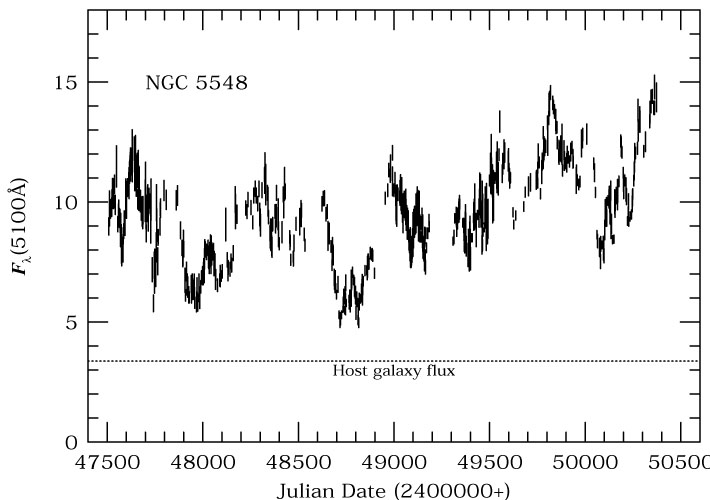
\includegraphics[scale=0.25]{images/NGC5548_Variability.jpg}
  \end{figure}
  \centering
    {\tiny \citep{Peterson99}}
  \begin{columns}
  \centering
    \begin{column}{0.5\textwidth}
      \begin{itemize}
        \item $\sim$ 90 \% vary {\tiny \citep{Sesar07}}
        \item Pan-spectral: shorter $\lambda \Rightarrow$ stronger variability
      \end{itemize}
    \end{column}
    \begin{column}{0.5\textwidth}
      \begin{itemize}
        \item Stochastic! {\tiny \citep{Peterson}}
        \item longer $\lambda$ lag shorter $\lambda$
      \end{itemize}
    \end{column}
  \end{columns}
\end{frame}

\begin{comment}

\subsection{Basic Facts About AGN}

\begin{frame}
\frametitle{Are these galaxies different?}
  \begin{figure}
    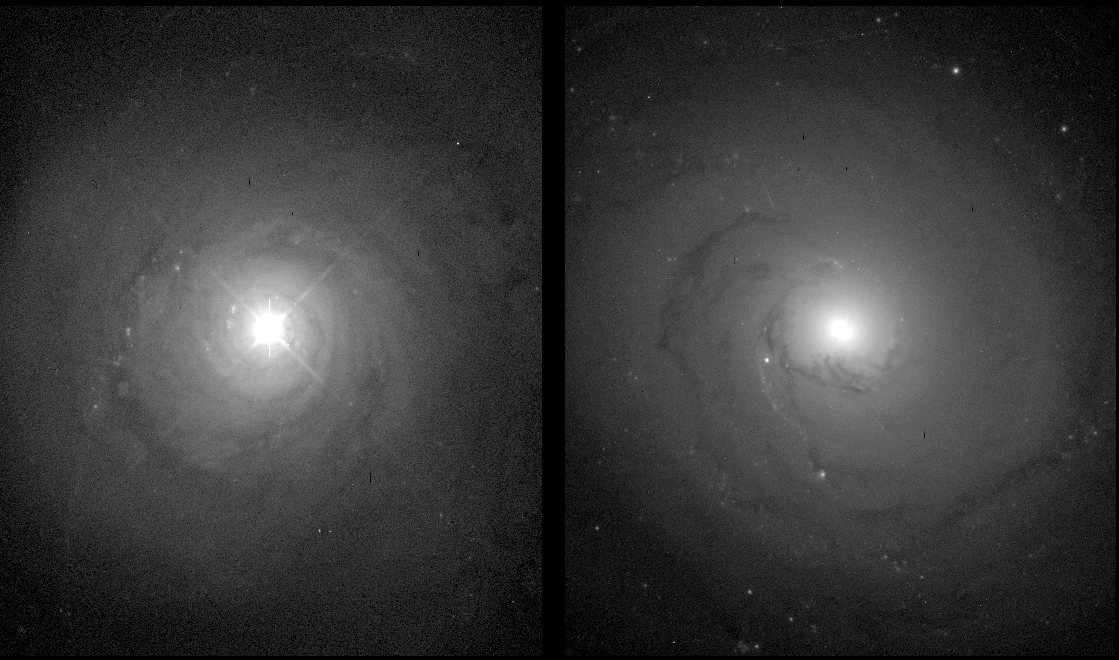
\includegraphics[scale=0.25]{./images/ngc5548.jpg}
  \end{figure}
  \begin{center}
  NGC 5548 (AGN Host) v/s NGC 3277 (non-AGN Host)
  \end{center}
\end{frame}

\begin{frame}
\frametitle{How bright can AGN be?}
  \begin{columns}
  \centering
    \begin{column}{0.5\textwidth}
      \begin{figure}
        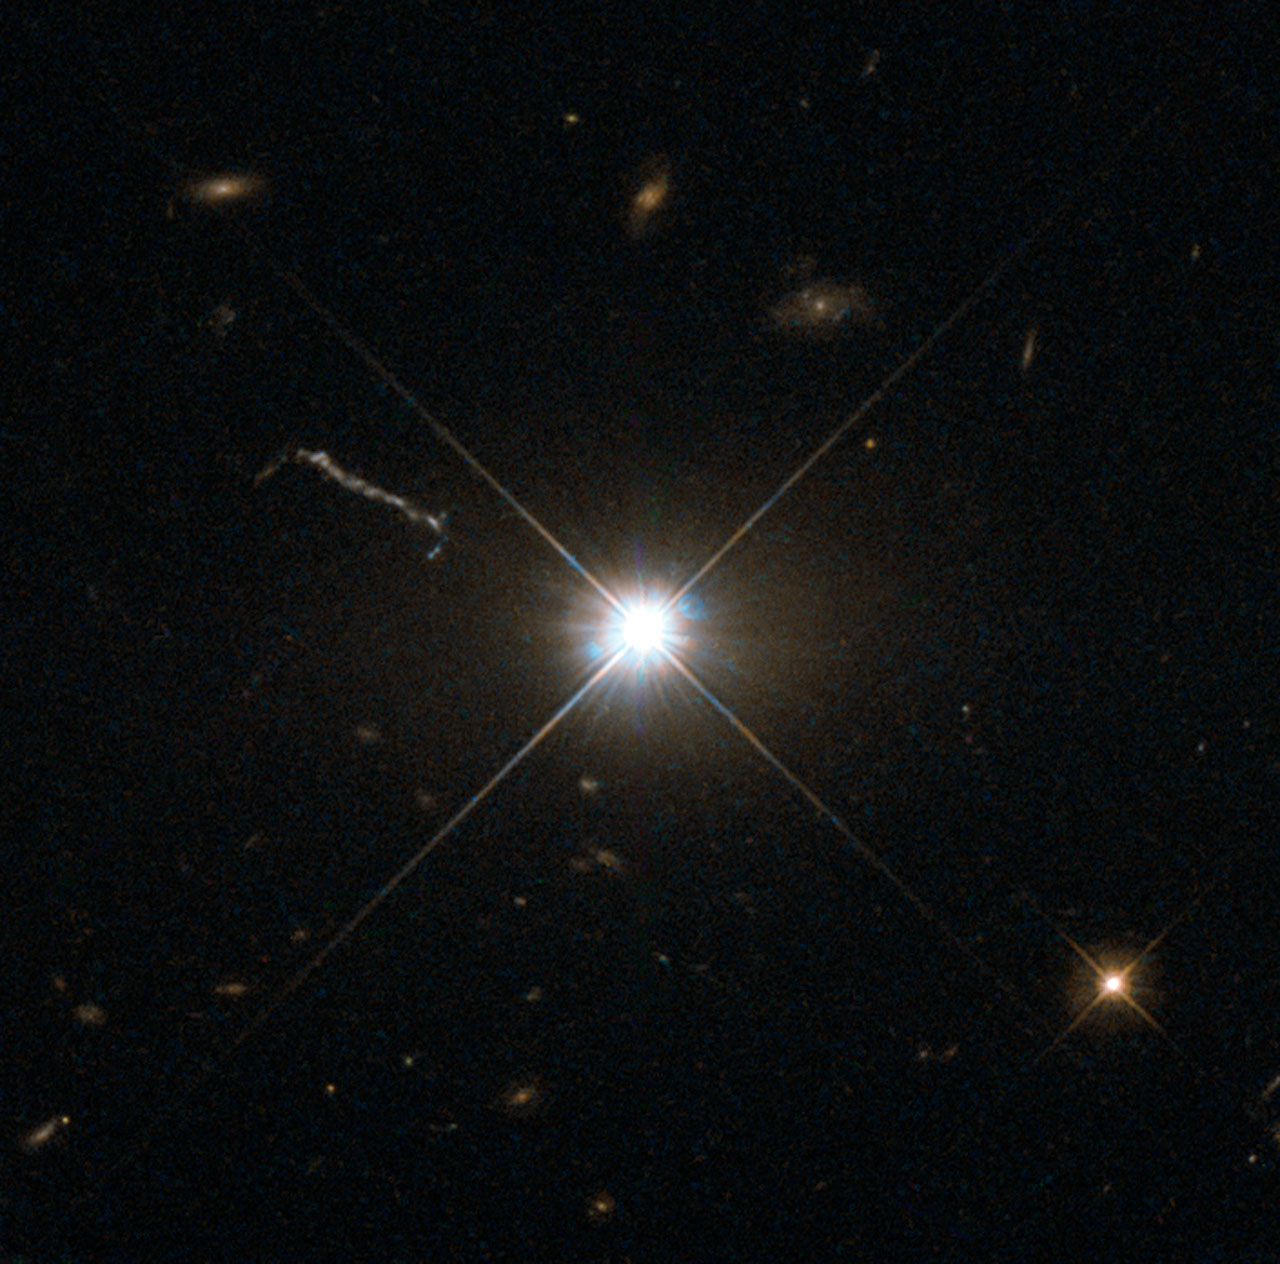
\includegraphics[scale=0.1]{./images/3C_273.jpg}
      \end{figure}
      3C 273 Completely Outshines Its Host Galaxy!
    \end{column}
    \begin{column}{0.5\textwidth}
      \begin{figure}
        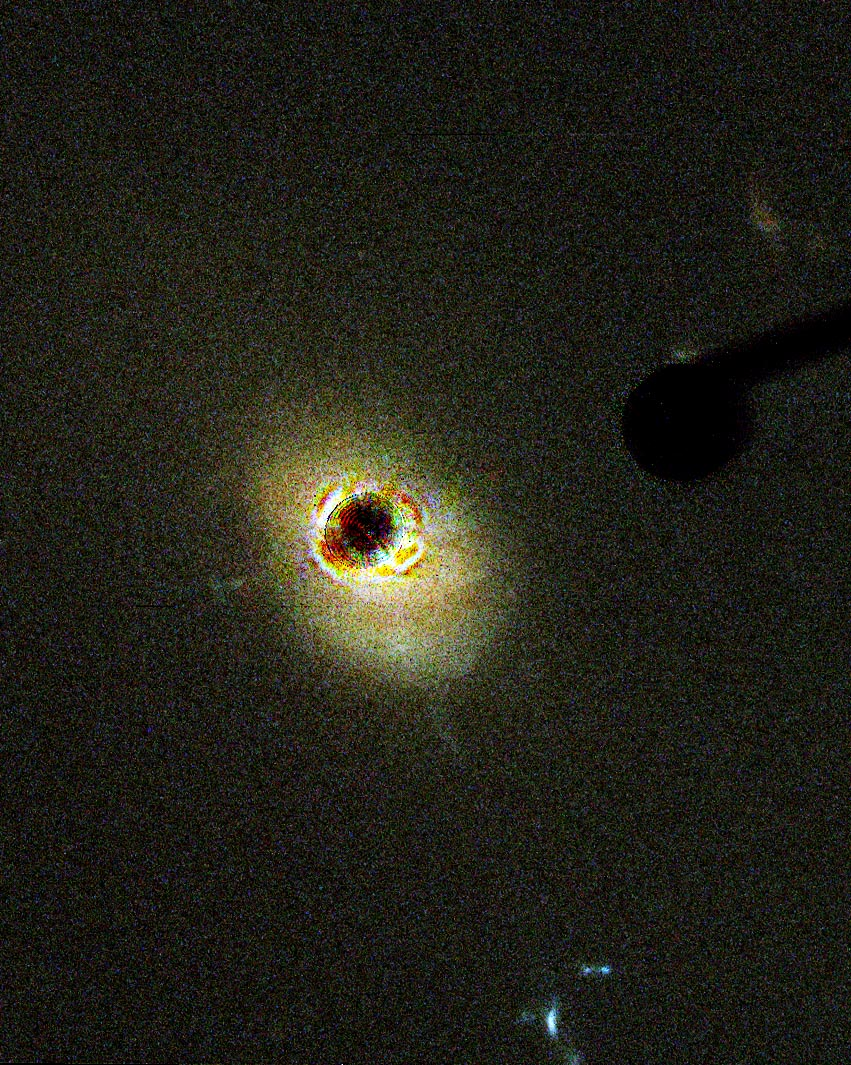
\includegraphics[scale=0.35]{./images/Quasar_3C_273.jpg}
      \end{figure}
    \end{column}
  \end{columns}
\end{frame}

\begin{frame}
\frametitle{So what is an AGN?\\In a nutshell...}
  \begin{figure}
    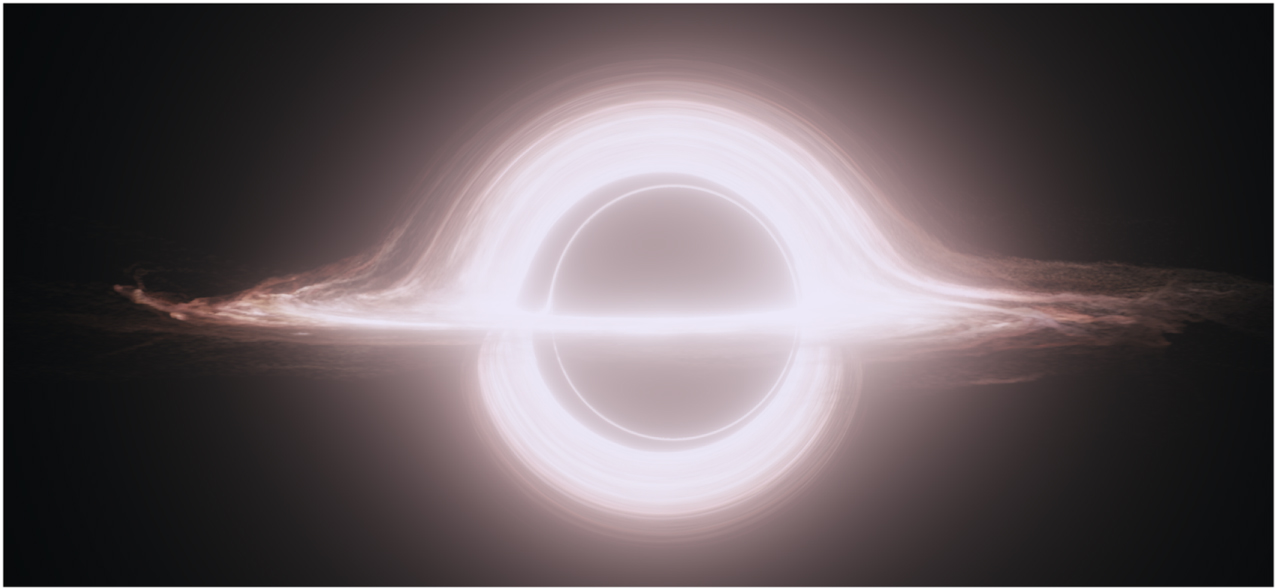
\includegraphics[scale=1.00]{./images/Gargantua_Paper2.jpg}
  \end{figure}
  \begin{center}
  {\tiny \citet*{Interstellar}}
  \end{center}
  ... but a lot less anemic!
\end{frame}

\begin{frame}
\frametitle{More realistically...}
  \begin{figure}
    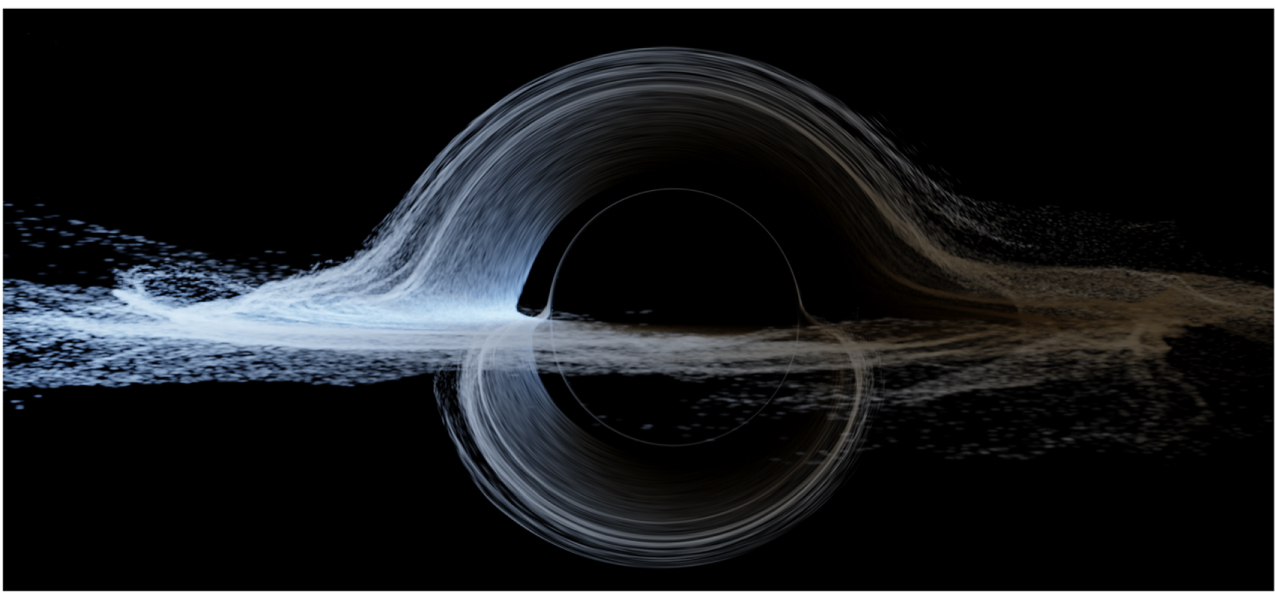
\includegraphics[scale=1.00]{./images/Gargantua_Paper3.jpg}
  \end{figure}
  \begin{center}
  {\tiny \citet*{Interstellar}}
  \end{center}
\end{frame}

\begin{frame}
\frametitle{How common are AGN?}
  \begin{figure}
    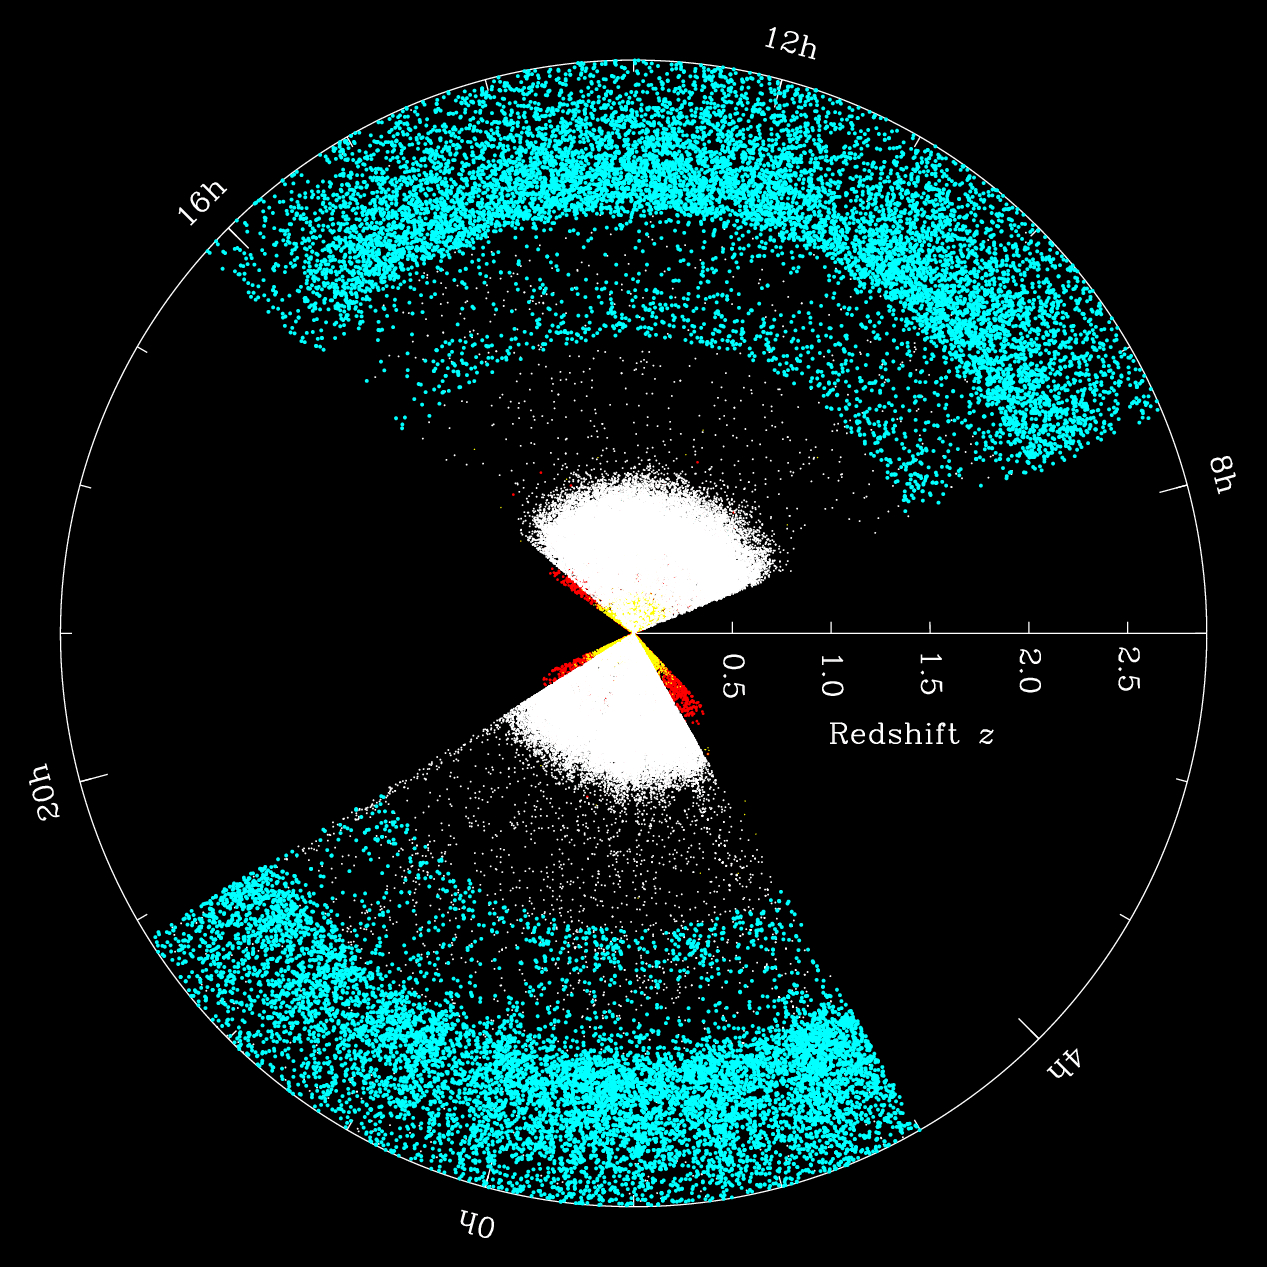
\includegraphics[scale=0.1]{./images/pie_boss_z2-900.jpg}
  \end{figure}
  \begin{center}
    \href{http://blog.sdss.org/wp-content/uploads/2011/11/pie_boss_z2-900.jpg}{{\tiny SDSS-III}}
  \end{center}
  \begin{columns}
  \centering
    \begin{column}{0.5\textwidth}
      \begin{itemize}
        \item $1$ in $50$ in local Universe.
        \item $\sim 120$~deg$^{2}$ at SDSS limit
      \end{itemize}
    \end{column}
    \begin{column}{0.5\textwidth}
      \begin{itemize}
        \item $\sim 10000$~deg$^{-2}$ in \textit{Chandra} 4Ms Survey {\tiny \citep{Netzer}}
        \item $1$ in $4$ including LINERS
      \end{itemize}
    \end{column}
  \end{columns}
\end{frame}

\begin{frame}
\frametitle{Do AGN dictate the evolution of galaxies?}
  \begin{columns}
    \centering
    \begin{column}{0.5\textwidth}
      \begin{figure}
        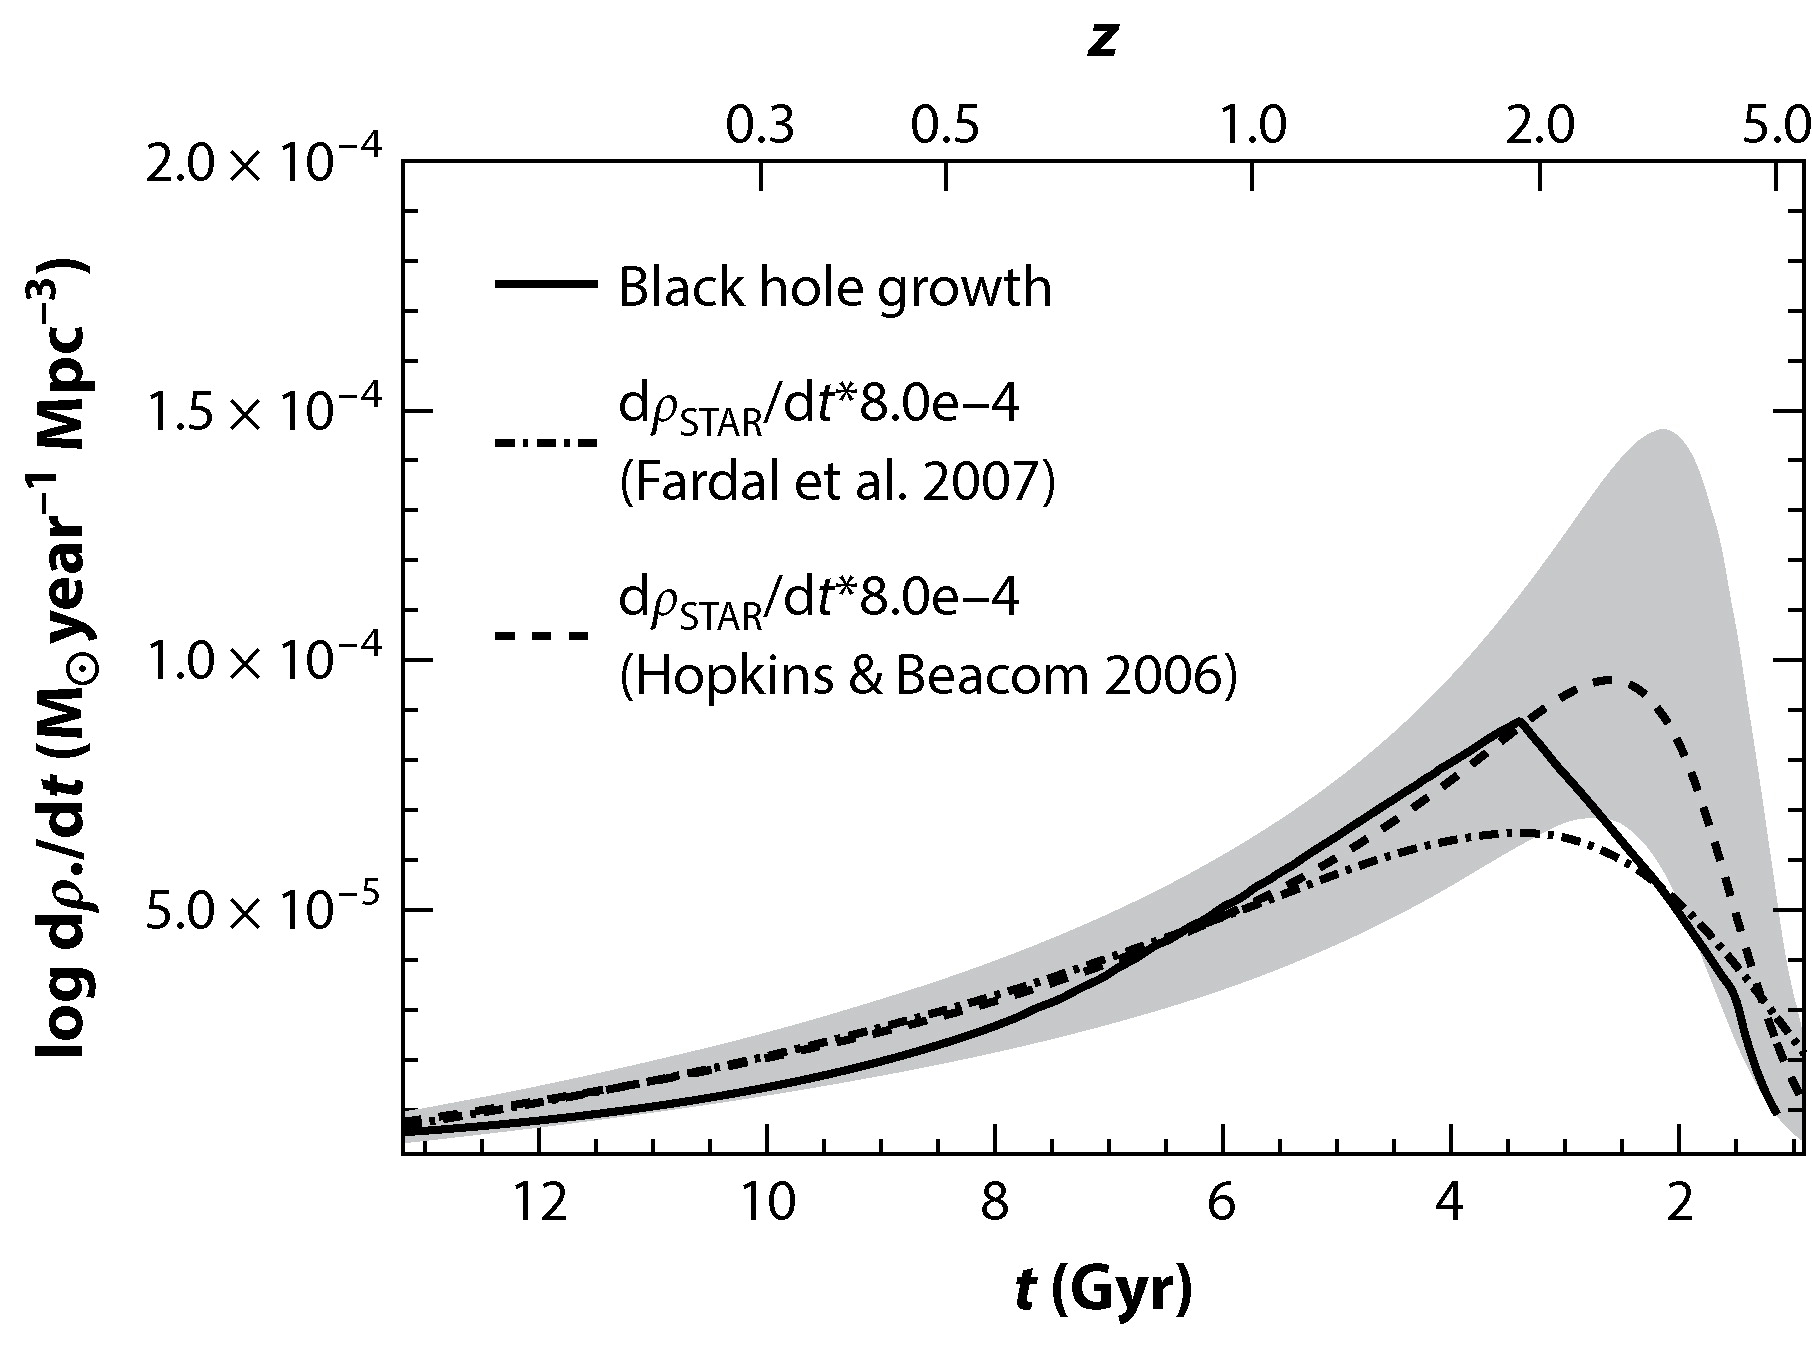
\includegraphics[scale=0.75]{./images/HeckmannBest.jpeg}
      \end{figure}
    \end{column}
    \begin{column}{0.5\textwidth}
      \begin{figure}
        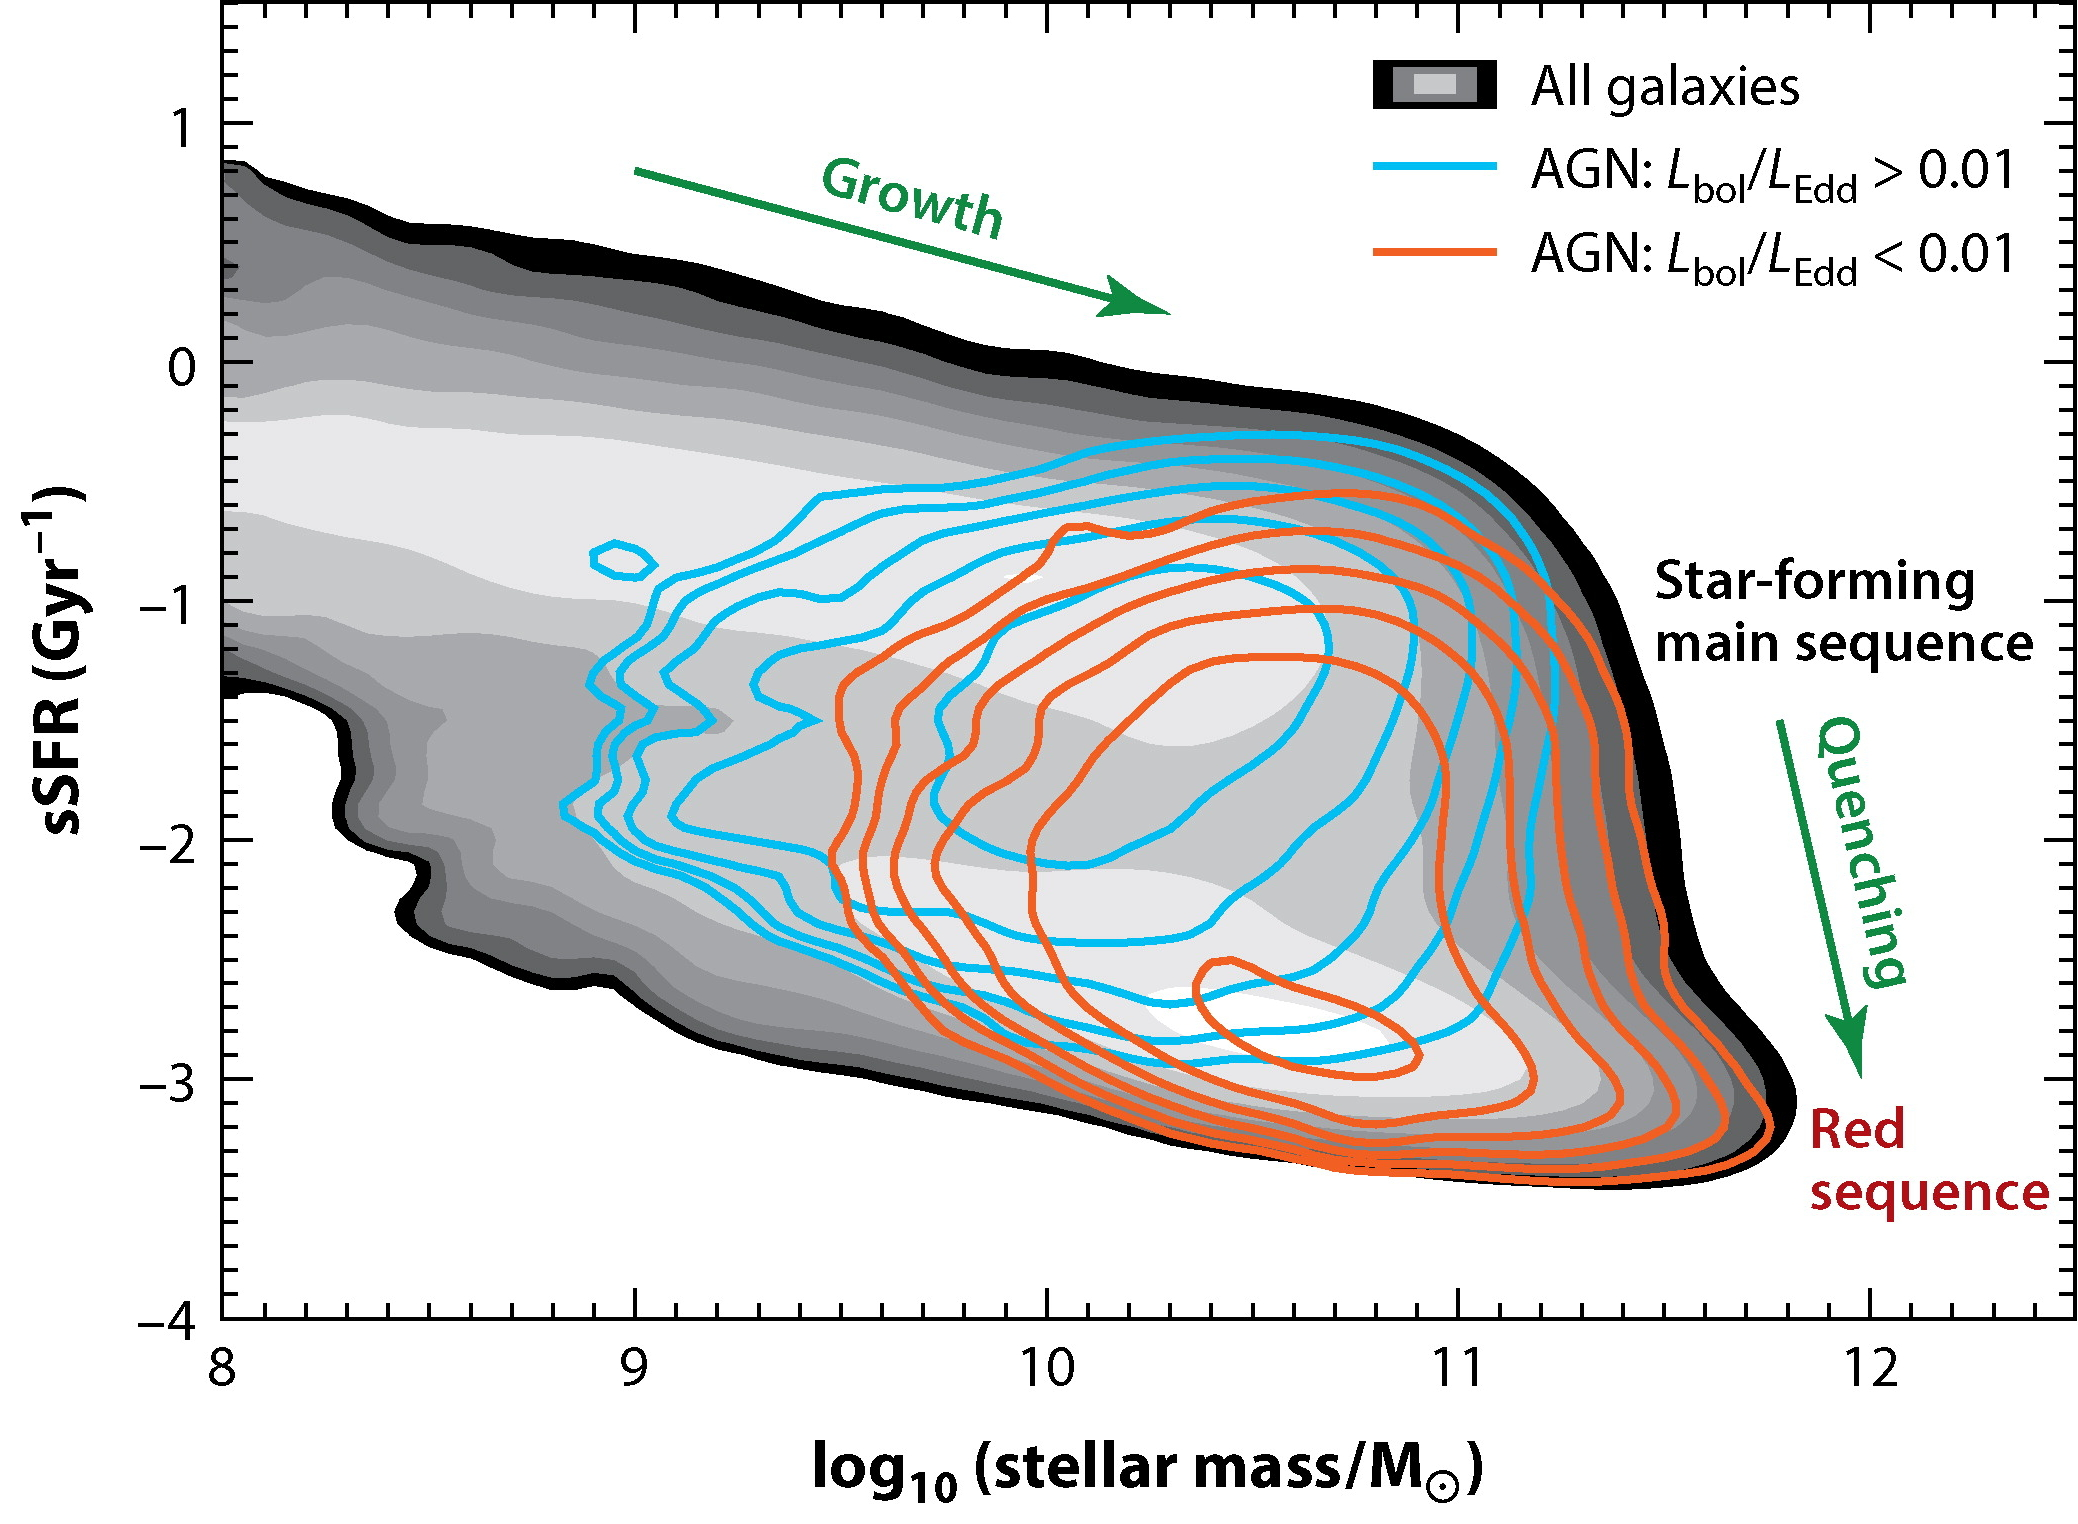
\includegraphics[scale=0.6]{./images/HeckmannBest2.jpeg}
      \end{figure}
    \end{column}
  \end{columns}
  \begin{center}
    {\tiny \citet{HeckmanBestARAA}}\\
    AGN quench star formation in galaxies!
  \end{center}
\end{frame}

\end{comment}

\begin{frame}
\frametitle{AGN Morphology: Continuum Variations $\rightarrow$ Origin in Accretion Disk}
  \begin{columns}
  \centering
    \begin{column}{0.5\textwidth}
      \begin{figure}
        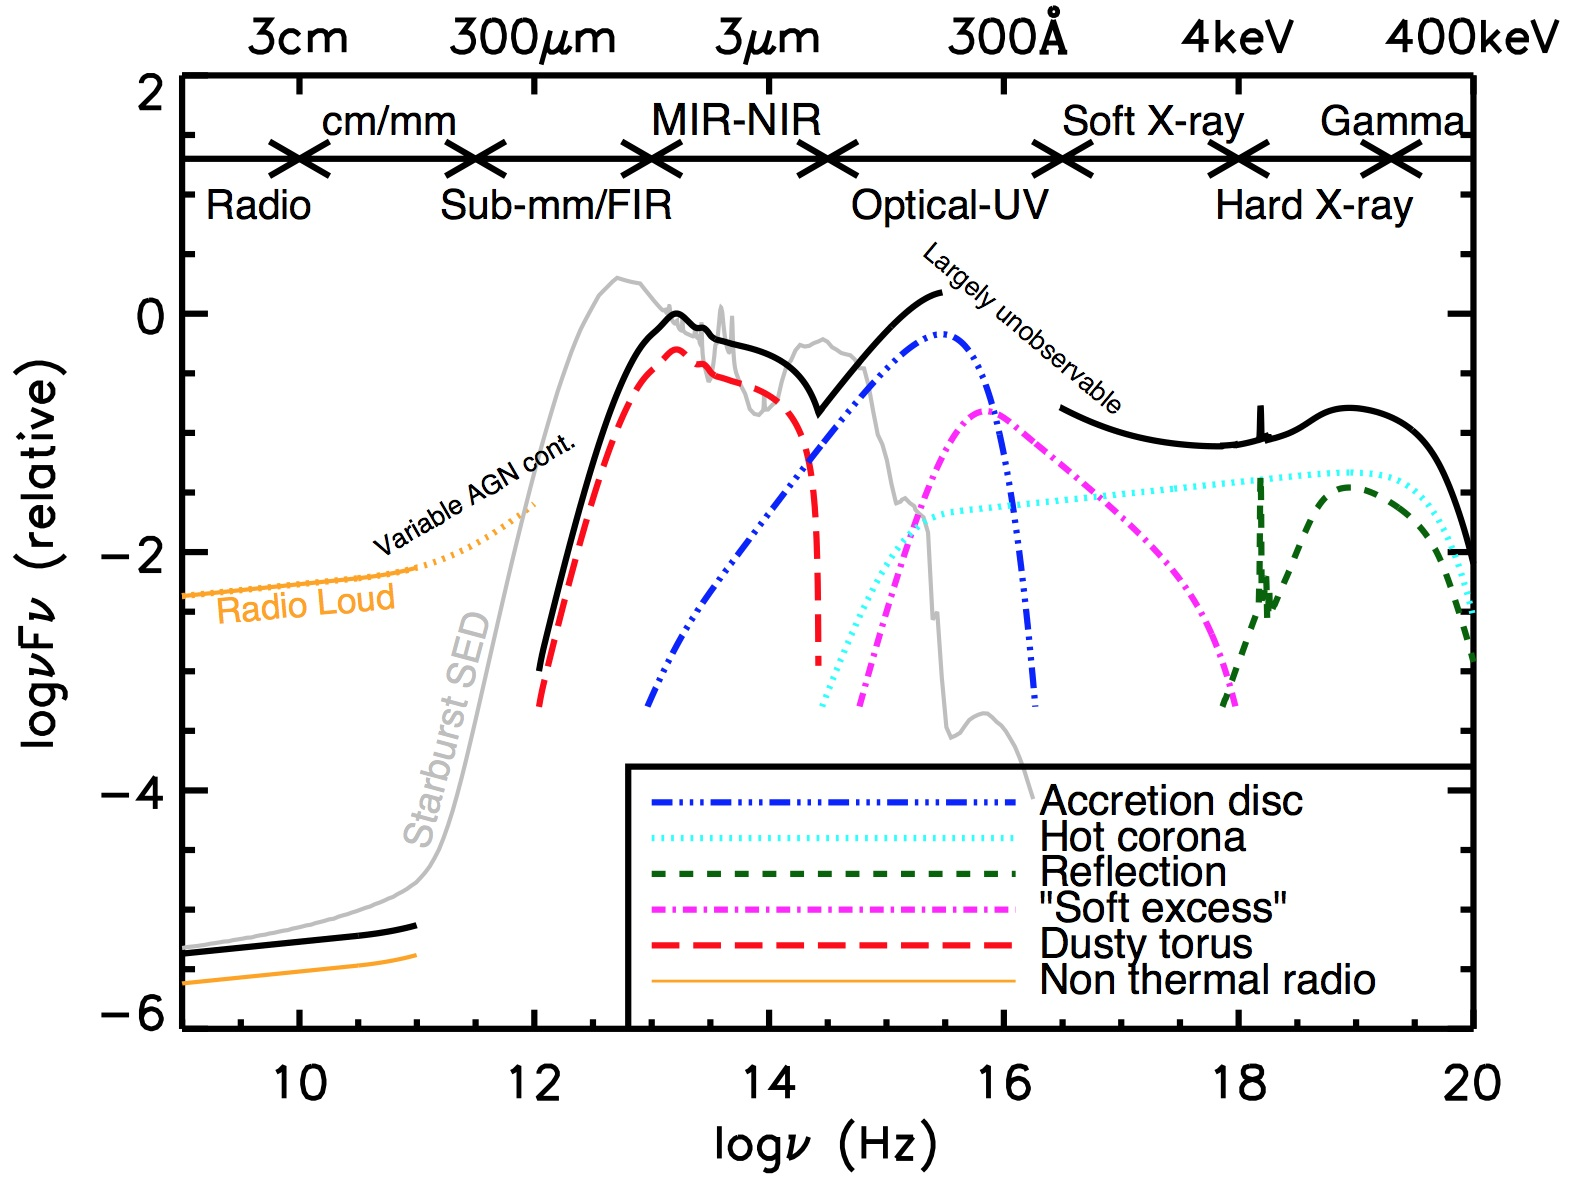
\includegraphics[scale=0.1]{images/agn_sed.jpg}
      \end{figure}
      \begin{center}
        %{\tiny \citet{Polletta07}}
        \href{http://astro.dur.ac.uk/~cpnc25/research.html}{{\tiny Chris Harrison}}
      \end{center}
    \end{column}
    \begin{column}{0.5\textwidth}
      \begin{figure}
        \includegraphics[scale=0.25]{images/AGNModel.jpg}
      \end{figure}
      %\begin{center}
        %{\tiny \citet{Peterson}}
        %\href{http://168.176.8.14/sagan/TipoAGN.html}{{\tiny Columbian National University: Bogota}}
      %\end{center}
    \end{column}
  \end{columns}
\end{frame}


\begin{comment}


\begin{frame}
\frametitle{Accretion Mechanism: The MRI}
  \begin{columns}
  \centering
    \begin{column}{0.5\textwidth}
      \begin{figure}
        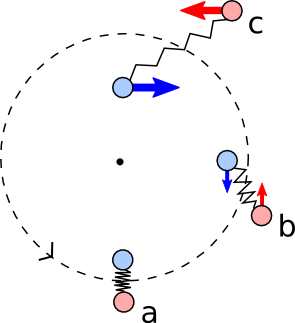
\includegraphics[scale=0.5]{images/MRI.jpg}
      \end{figure}
      \begin{center}
        %{\tiny \citet{Polletta07}}
        \href{https://ay201b.wordpress.com/2011/04/11/the-magnetorotational-instability/}{{\tiny Harvard Astronomy Dept}}
      \end{center}
    \end{column}
    \begin{column}{0.5\textwidth}
      %\begin{figure}
        %\includegraphics[scale=0.25]{../images/talk/AGNModel.jpg}
      %\end{figure}
      \movie[externalviewer]{\includegraphics[scale=0.5]{images/pol3d.jpg}}{disk04a.mpg}
      %\movie[autostart,showcontrols=true]{\includegraphics[scale=0.5]{../images/talk/pol3d.jpg}}{disk04a.mpg}
      \begin{center}
        {\tiny \citet{HawleyKrolik02}}
        %\href{http://168.176.8.14/sagan/TipoAGN.html}{{\tiny Columbian National University: Bogota}}
      \end{center}
    \end{column}
  \end{columns}
\end{frame}

\begin{frame}
\frametitle{Sources of variability}
  \begin{columns}
    \begin{column}{0.5\textwidth}
      \begin{center}
        \centering
        \movie[externalviewer]{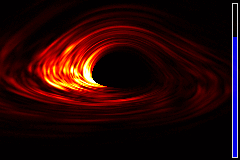
\includegraphics[scale=0.5]{images/fluctuations.jpg}}{flyby_large.mpg}
      \end{center}
      \begin{center}
        \centering
        {\tiny \citet{ArmitageReynolds03}}
      \end{center}
      Magnetic Reynolds number: $R_{\mathrm{magnetic}} = UL/\eta \ \sim$ advection vs diffusion. \\
      Magnetic diffusivity $\eta = \frac{m_{\mathrm{e}}\nu_{\mathrm{collision}}}{\mu_{0}\mathrm{n}_{\mathrm{e}}\mathrm{e}^{2}}$.
    \end{column}
    \begin{column}{0.5\textwidth}
      \begin{itemize}
        \item $\lambda$ dependent (X-Ray partially drives Optical) {\tiny \citep{UttleyAccretion}}
        \item Shot noise models unlikely {\tiny \citep{UMV05}}
        \item MHD turbulence responsible {\tiny \citep{NowakWagoner95}}
        \item Coronal X-Ray flares possible {\tiny \citep{PoutanenFabian99}}
        \item Propagating fluctuations {\tiny \citep{Lyubarskii97}}
          \begin{itemize}
            \item Predicts PSD
          \end{itemize}
        \item Coronal accretion {\tiny \citep{JaniukCzerny07}}
      \end{itemize}
    \end{column}
  \end{columns}
\end{frame}

\begin{frame}
\frametitle{Timescales that \textit{may} be found in AGN}
  \begin{figure}
    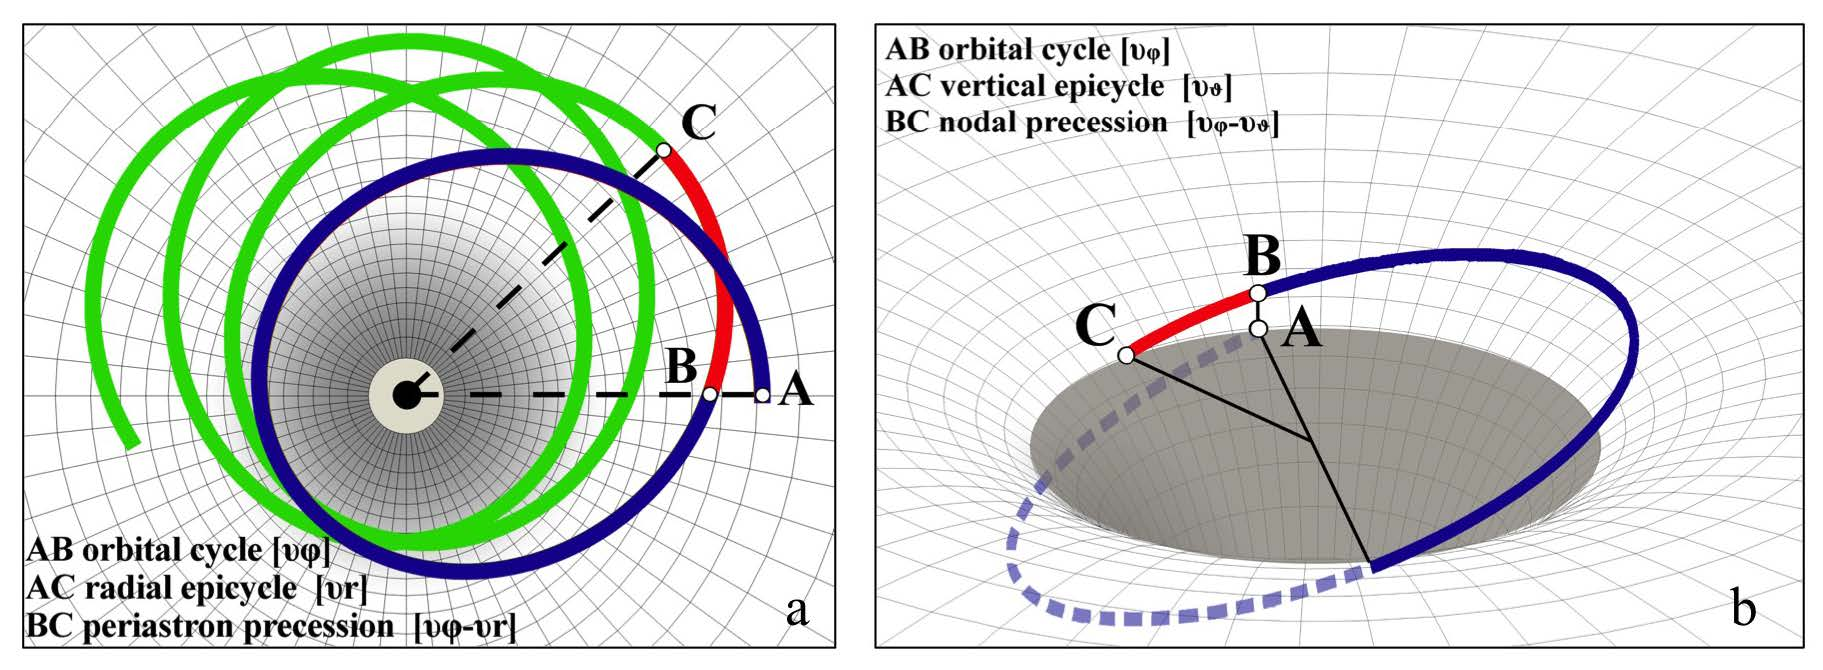
\includegraphics[scale=0.55]{images/BelloniStella14_KerrOrbits.jpg}
  \end{figure}
  \centering
  {\tiny \citet{BelloniAccretion}}
  \begin{columns}
    \begin{column}{0.6\textwidth}
      \begin{itemize}
        \item $t_{\mathrm{dyn}} = \sqrt{\frac{r^{3}}{G \mathrm{M}_{\mathrm{BH}}}} \sim 1$-$1500$~d
      \end{itemize}
    \end{column}
    \begin{column}{0.4\textwidth}
      \begin{itemize}
        \item $t_{\mathrm{therm}} = \frac{t_{\mathrm{dyn}}}{\alpha} \sim 1$~d - $5$~yr
      \end{itemize}
    \end{column}
  \end{columns}
  \begin{itemize}
    \centering
    \vspace{5mm}
    \item $t_{\mathrm{visc}} = \frac{t_{\mathrm{dyn}}}{\alpha(H/r)^{2}} \sim 1$-$10$~yr
  \end{itemize}
\end{frame}

\begin{frame}
\frametitle{Search for timescales in Power Spectral Density (PSD)}
  \begin{center}
    \centering
        \begin{figure}
          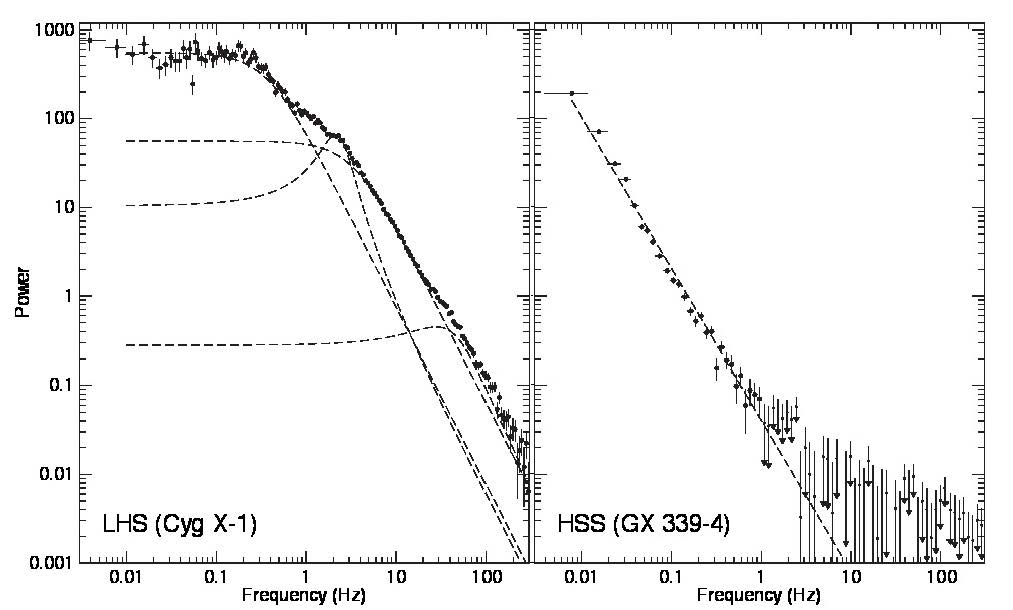
\includegraphics[scale=0.75]{images/BelloniStella14_PDS.jpg}
        \end{figure}
  \end{center}
  \begin{center}
    \centering
    {\tiny \citet{BelloniAccretion}}
  \end{center}
\end{frame}

\subsection{The Damped Random Walk}

\begin{frame}
\frametitle{\citet{Kelly09}: Model variability as DRW}
  \begin{columns}
    \begin{column}{0.6\textwidth}
      \begin{center}
        \begin{figure}
          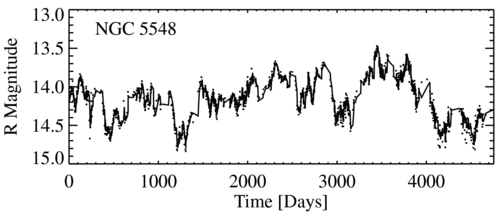
\includegraphics[scale=0.4]{images/Kelly09a.jpg}
        \end{figure}
      \end{center}
    \end{column}
    \begin{column}{0.4\textwidth}
        \begin{figure}
          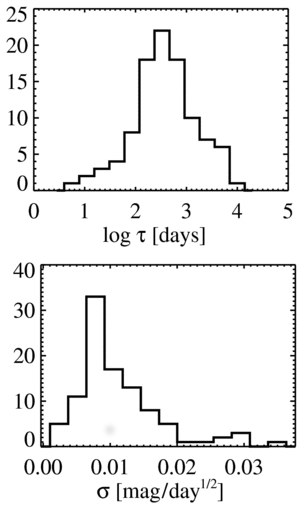
\includegraphics[scale=0.3]{images/Kelly09bf.jpg}
        \end{figure}
    \end{column}
  \end{columns}
  %\centering
  %{\tiny \citet{Kelly09}}
  \begin{itemize}
    \item Dynamical or thermal processes responsible for variability
    \item $\tau \propto \mathrm{M}_{\mathrm{BH}}$ \& $L_{\mathrm{AGN}}$ but $\sigma \propto 1/\mathrm{M}_{\mathrm{BH}}$ \& $1/L_{\mathrm{AGN}}$
  \end{itemize}
\end{frame}

\begin{frame}
\frametitle{PSD of the Damped Random Walk}
  \begin{columns}
    \centering
    \begin{column}{0.5\textwidth}
    \centering
    %{\tiny $\tau = 100$ d}
      \begin{figure}
        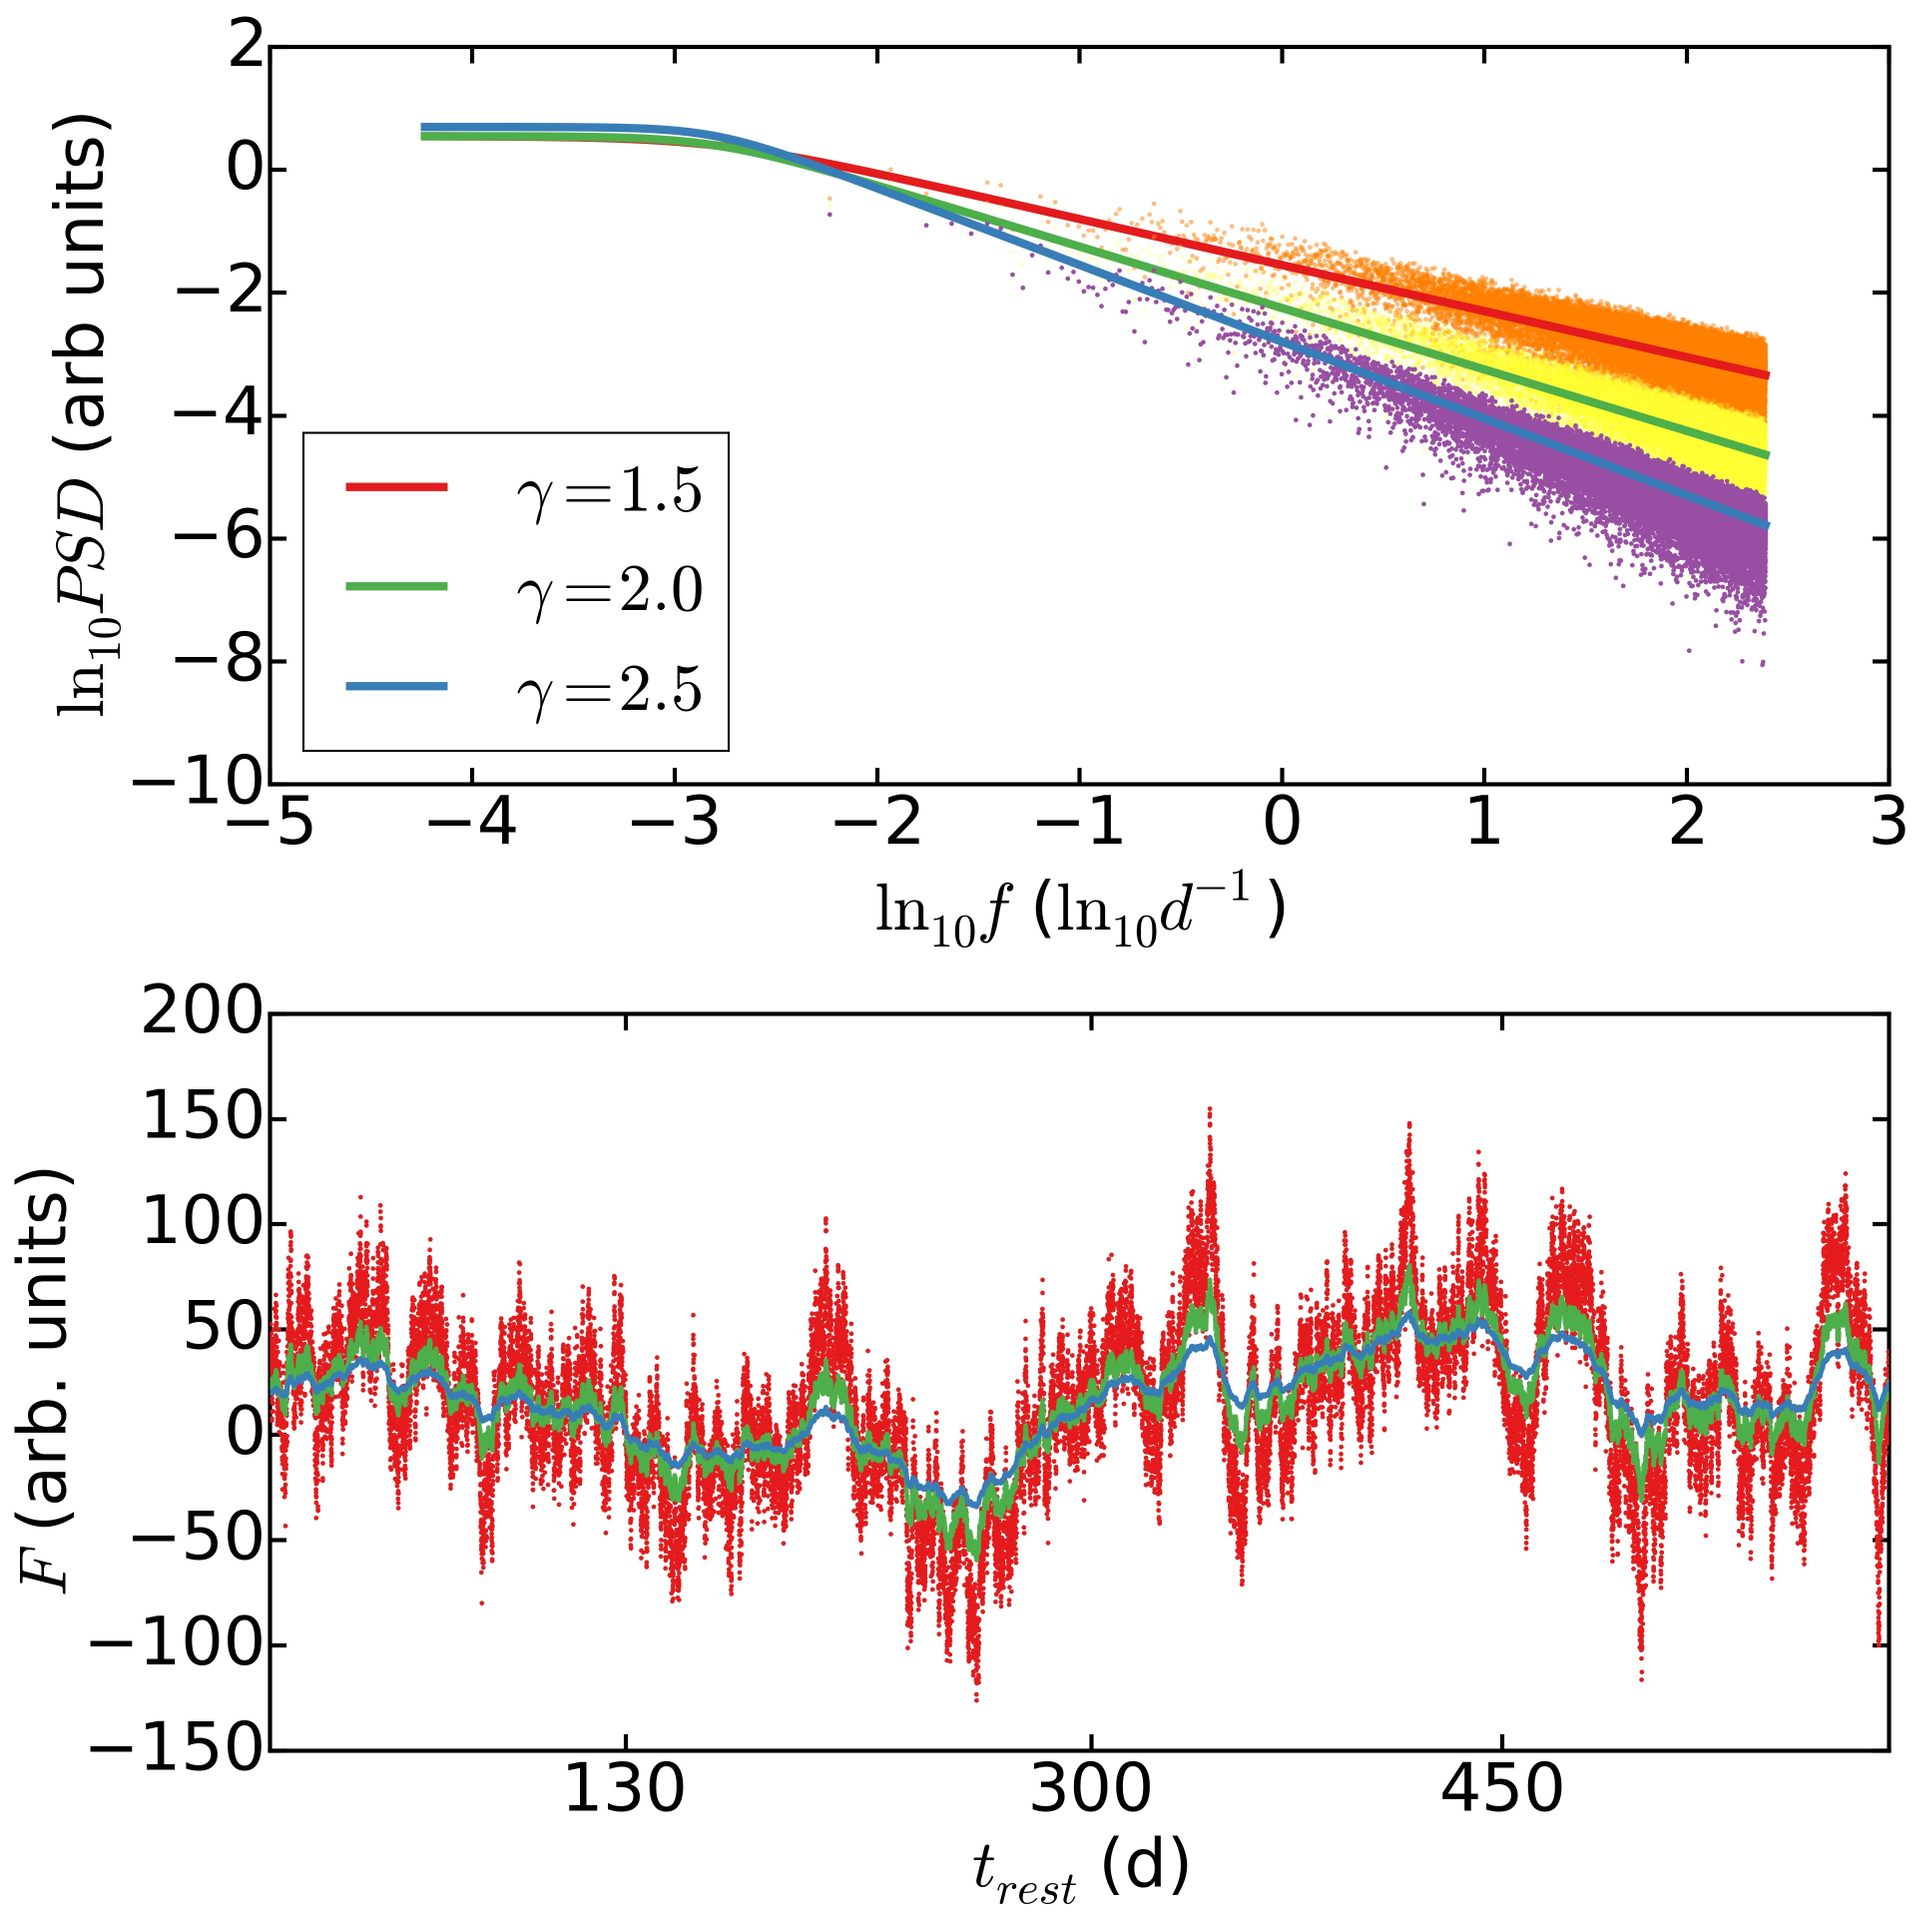
\includegraphics[scale=0.09]{images/DRW.jpg}
      \end{figure}
    \end{column}
    \begin{column}{0.5\textwidth}
    \begin{itemize}
    %\item $PSD(f) = \frac{\sigma^{2}}{1 + (2 \pi \tau f)^{2}} \propto \frac{1}{f^{2}}$ on short timescales.
    \item $PSD \propto \frac{1}{f^{2}}$ on short timescales
      %\pause
    \item $PSD \propto \frac{1}{f^{b}} \Rightarrow \sigma_{\alpha-fluc} \propto r^{b}$ {\tiny \citep{Lyubarskii97}}
      %\pause
    \item DRW: $b$ is fixed - is this true?
      %\pause
    %\item Generalize short timescale PSD: $PSD(f) = \frac{\sigma^{2}}{1 + (2 \pi \tau f)^{\gamma}}$ {\tiny \citep{mac04}}.
    \item Generalize: $PSD \propto \frac{1}{f^{\gamma}}$ {\tiny \citep{McHardy04}}
      %\pause
    \item Test with data!
    \end{itemize}
    \end{column}
  \end{columns}
\end{frame}

\begin{frame}
\frametitle{Serendipitous AGN science with Kepler}
  \begin{center}
    \centering
        \begin{figure}
          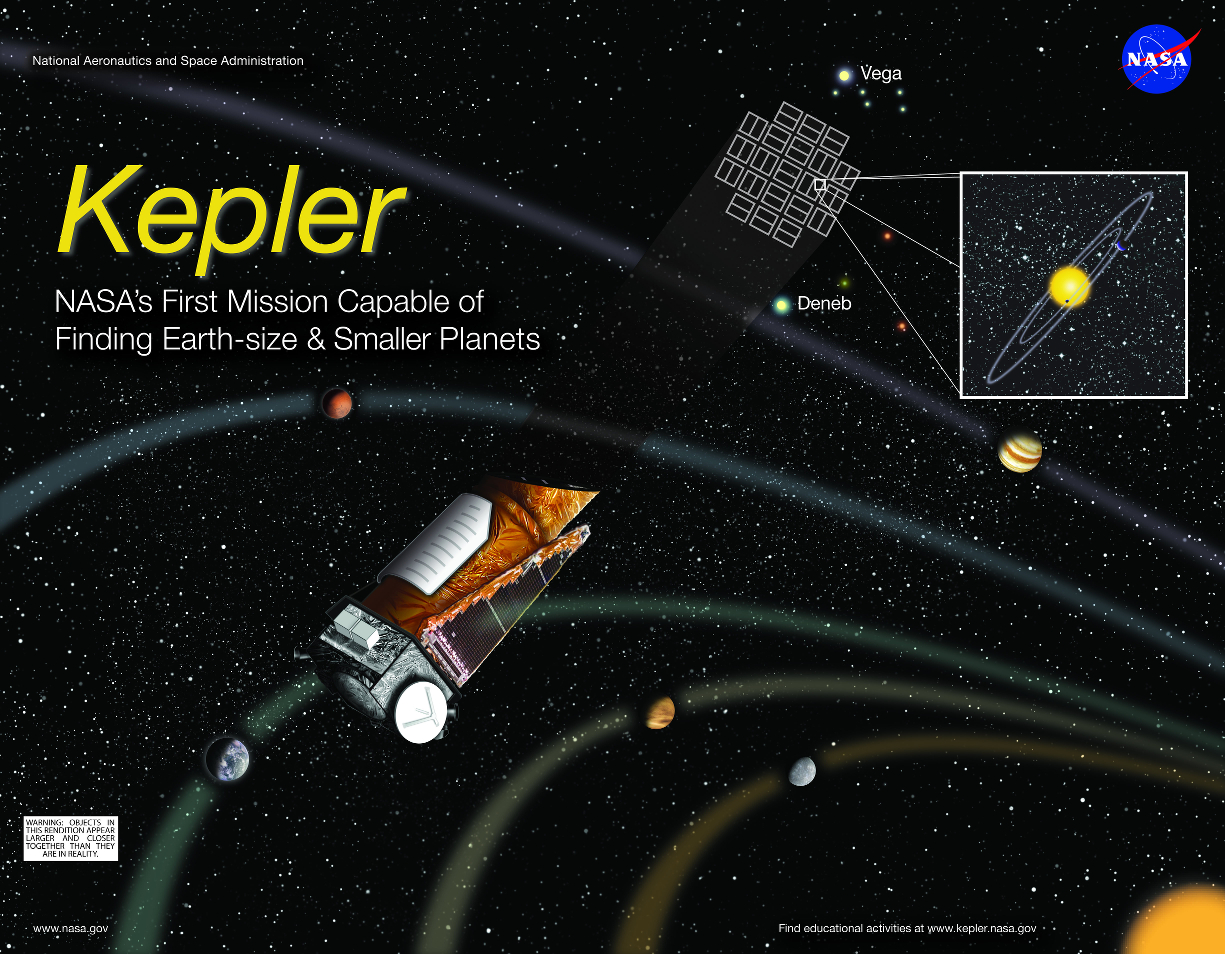
\includegraphics[scale=0.75]{images/Kepler_PosterMedium.jpeg}
        \end{figure}
  \end{center}
\end{frame}

\begin{frame}
\frametitle{Kepler Instrument Design}
  \begin{columns}
    \begin{column}{0.6\textwidth}
      \begin{center}
        \centering
        \begin{figure}
          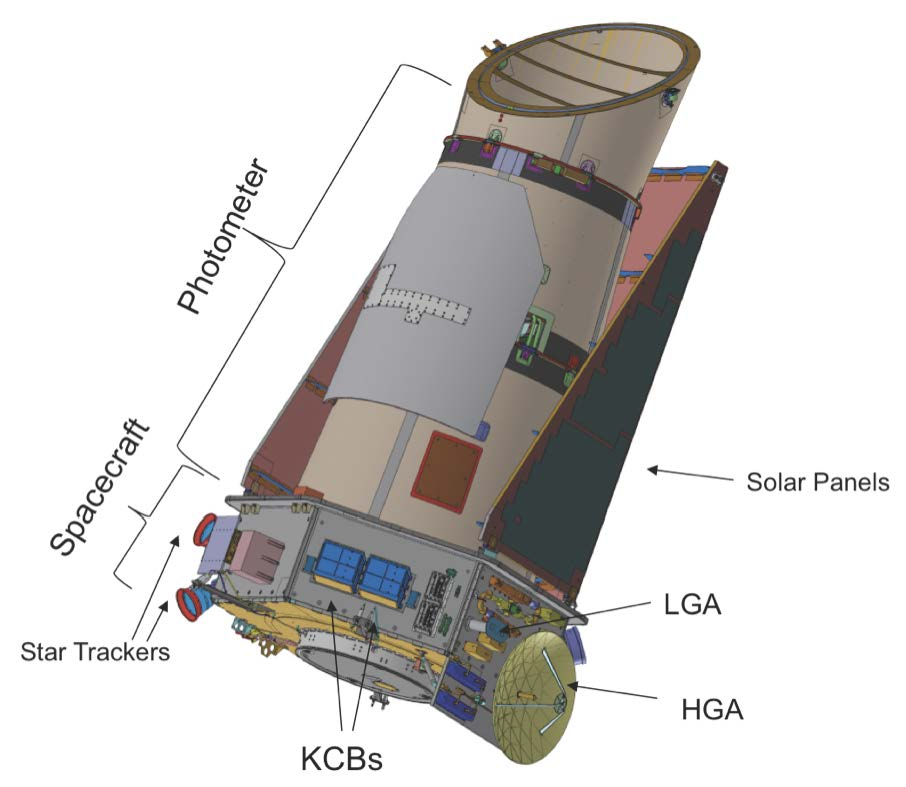
\includegraphics[scale=0.5]{images/Kepler_Spacecraft.jpg}
        \end{figure}
      \end{center}
    \end{column}
    \begin{column}{0.4\textwidth}
      \begin{itemize}
        \item Schmidt camera
        \item $0.95$~m clear aperture
        \item Fast f/$1.473$ optics
        \item Plate scale $3.98$~arcsec/pixel
        \item PSF: $95$-percent EED $\sim 6.4$~pixel
        \item Photometric Precision: 35 ppm (mag $12$ star)
      \end{itemize}
    \end{column}
  \end{columns}
\end{frame}

\begin{frame}
\frametitle{What can we learn from Kepler?}
\begin{columns}
\centering
  \begin{column}{0.5\textwidth}
    \begin{figure}
      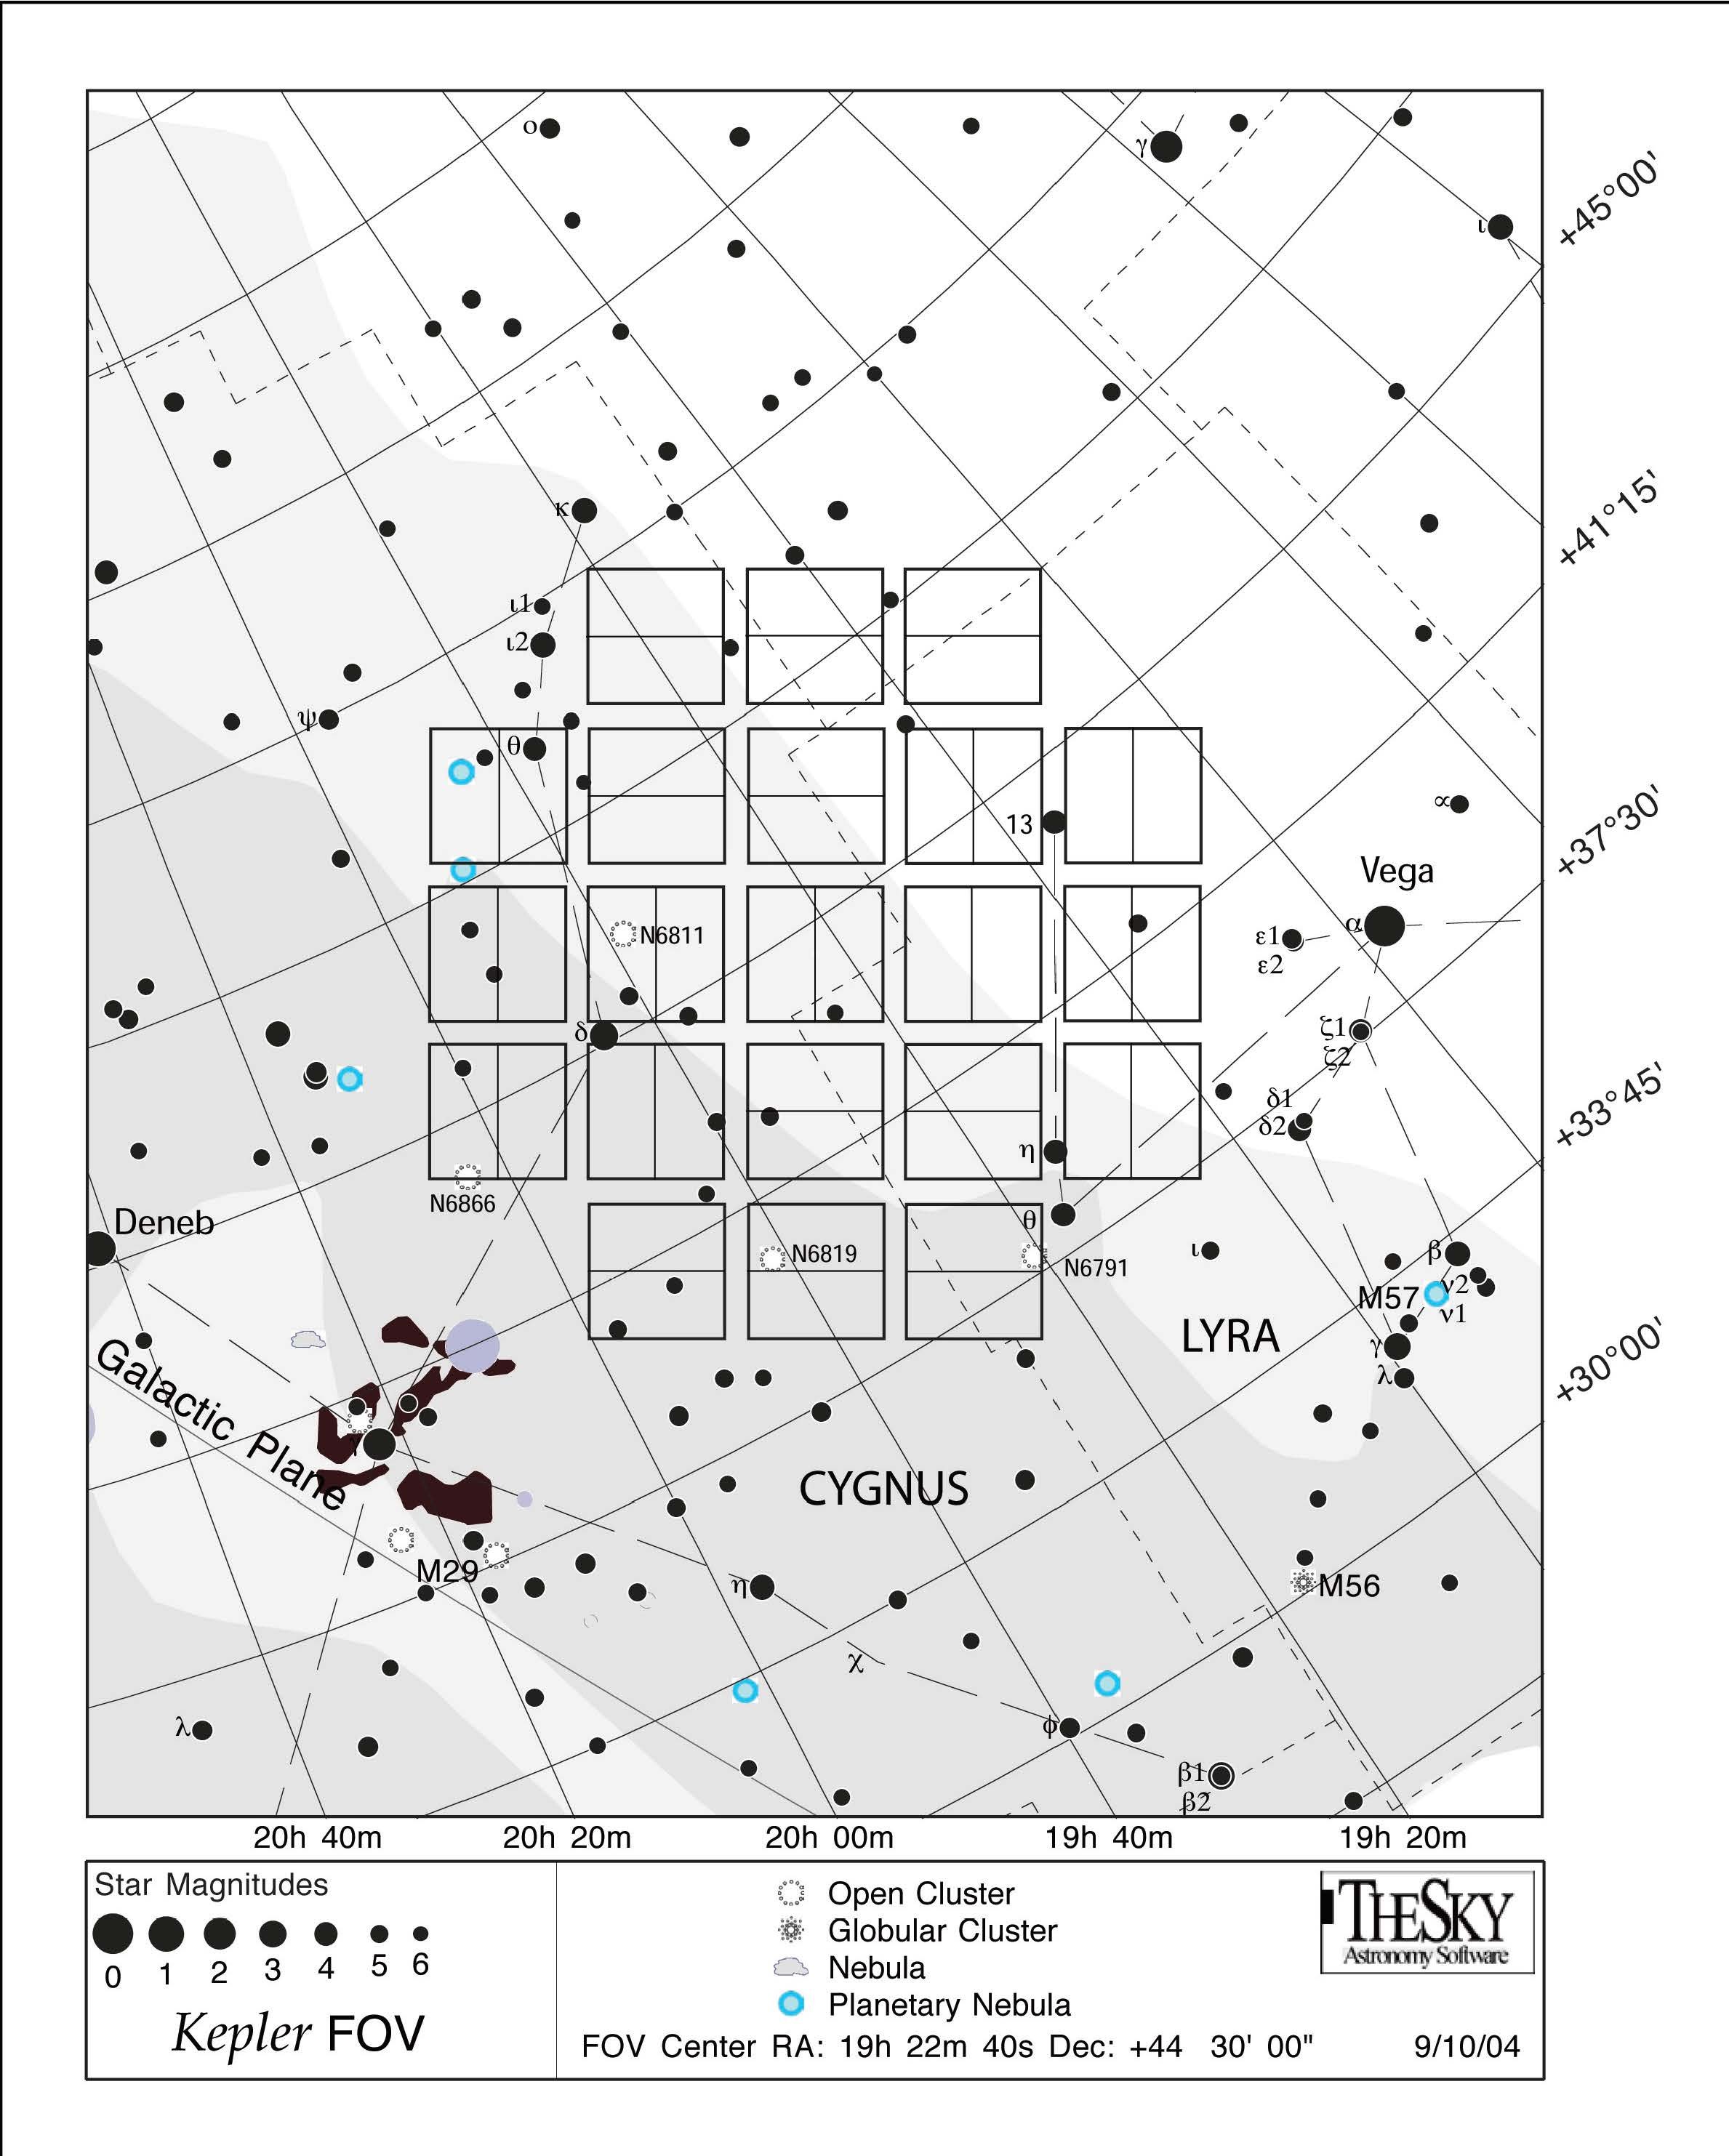
\includegraphics[scale=0.3]{images/Kepler_FOV.jpg}
    \end{figure}
      \centering
      {\tiny \citet{KIH}}
    \end{column}
    \begin{column}{0.5\textwidth}
        \begin{itemize}
        \item Very precise: S/N $\sim 10^{5}$
        \item Long baseline: $T = 3.5$~yr
        \item Rapid sampling: $\delta t_{\mathrm{obs}} = 29.4$~min
        \item $110$~deg$^{2}$ FOV
        \item $\sim 80$ AGN \\ {\tiny \citep{Mushotzky11,Edelson12,Carini12,Wehrle13,Shaya15}}
      \end{itemize}
    \end{column}
  \end{columns}
  \begin{center}
  \end{center}
\end{frame}


\end{comment}


\begin{frame}
\frametitle{AGN Show Complex Variability Behavior}
  \begin{columns}
    \centering
    \begin{column}{0.35\textwidth}
      \begin{figure}
        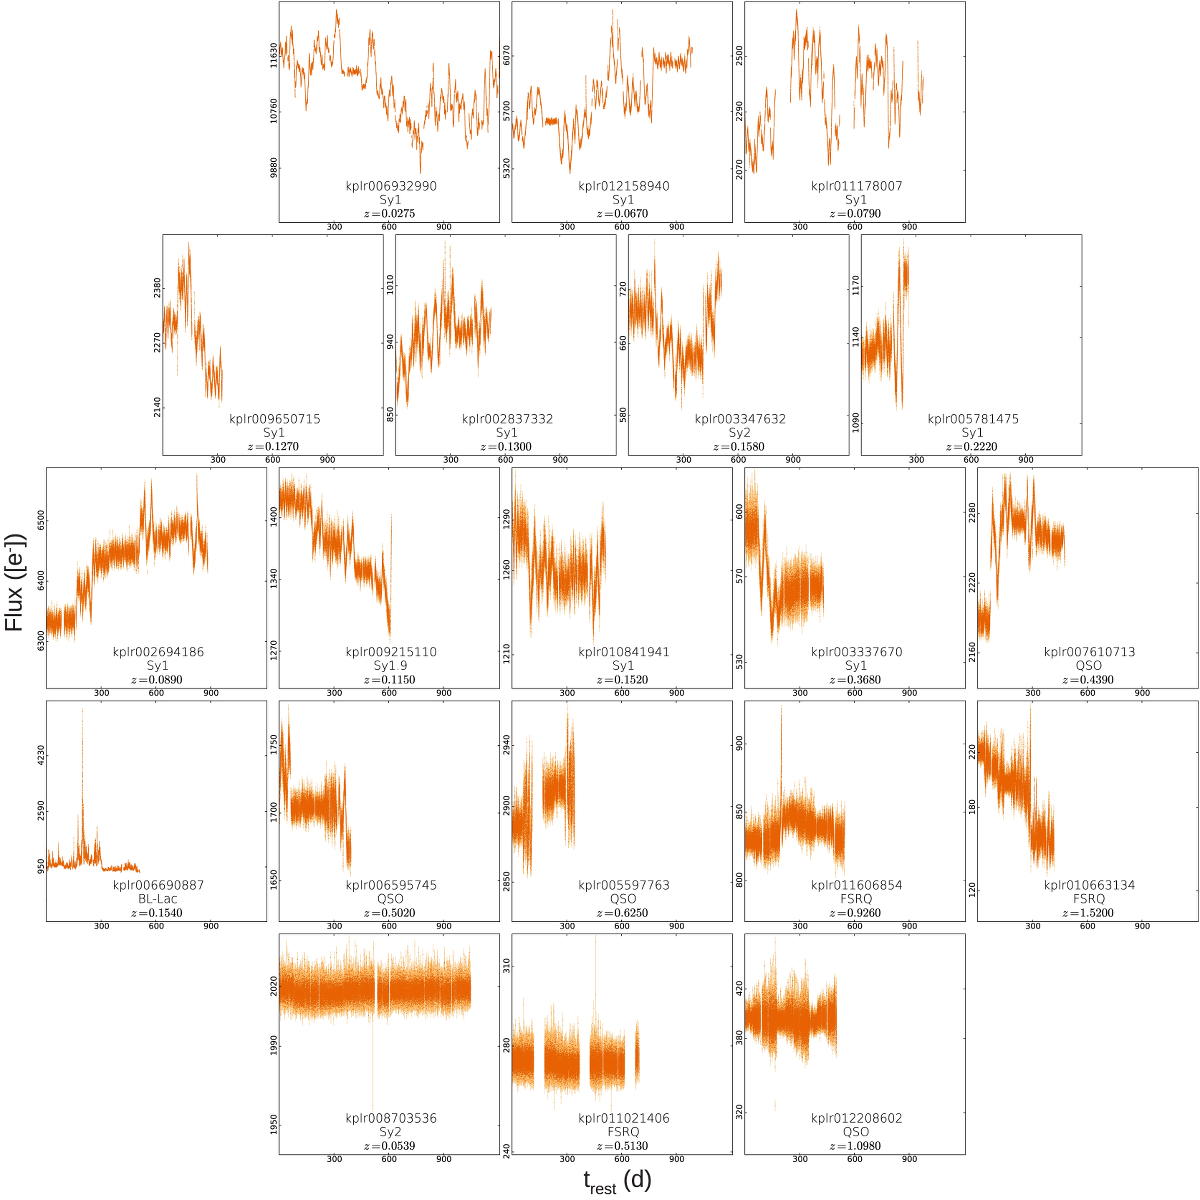
\includegraphics[scale=0.32]{images/AllLC.jpg}
      \end{figure}
    \end{column}
    \begin{column}{0.35\textwidth}
        \begin{figure}
          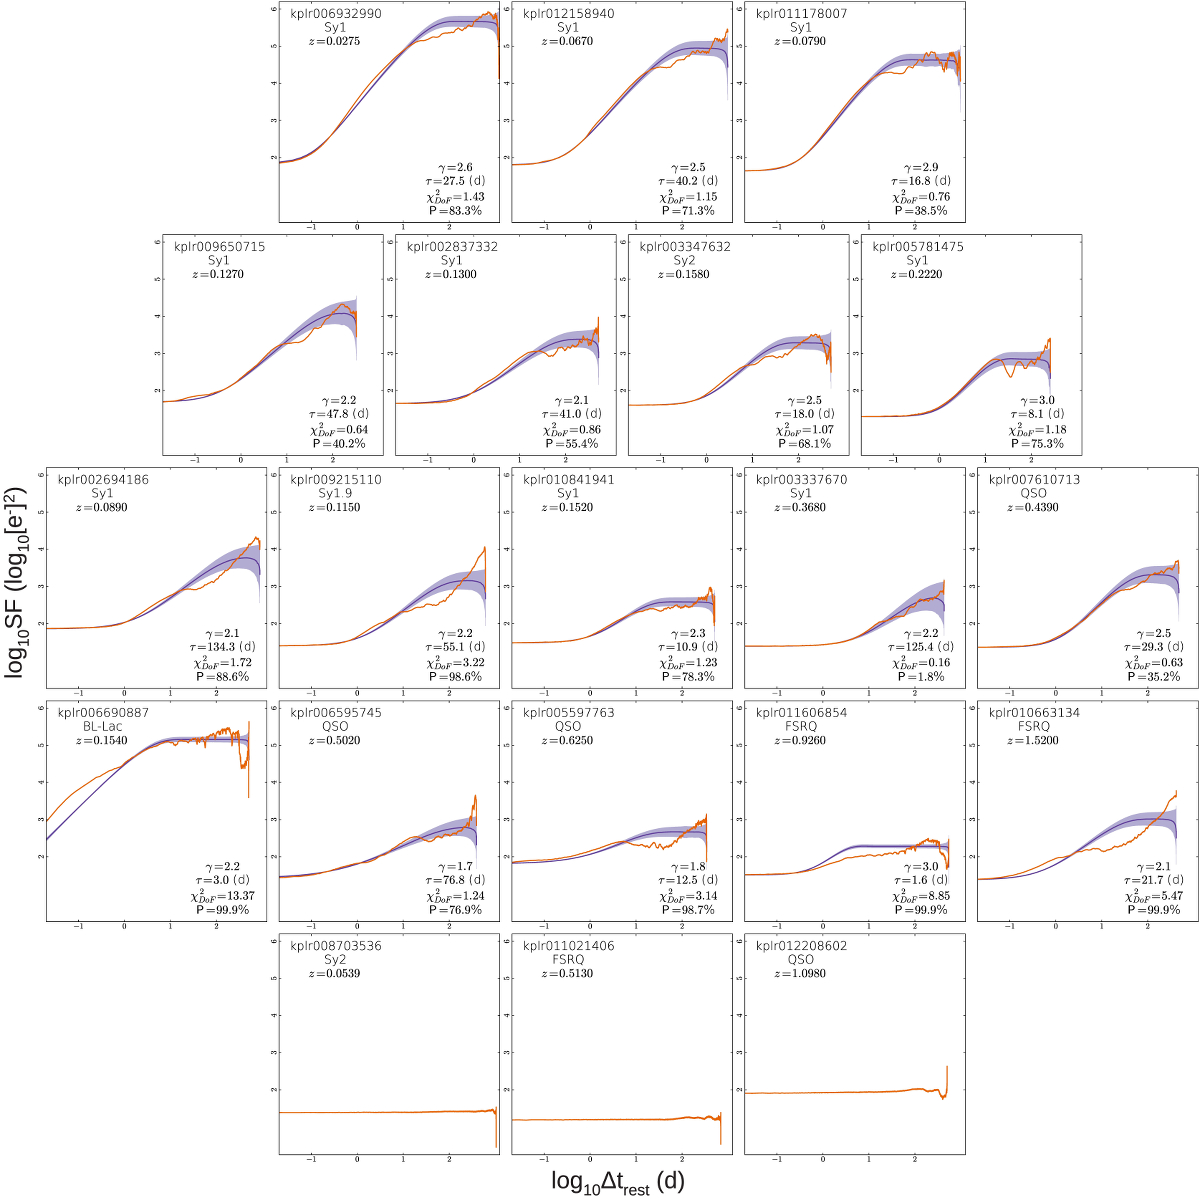
\includegraphics[scale=0.32]{images/AllSF.jpg}
        \end{figure}
    \end{column}
  \end{columns}
  \begin{columns}
    \centering
    \begin{column}{0.35\textwidth}
      \begin{itemize}
        \item {\footnotesize $z \sim 0.02$-$1.5$}
        \item {\footnotesize $\delta t_{\mathrm{rest}} \sim 14$-$28$~min}
        \item {\footnotesize $N \sim 16$k-$60$k}
        %\item Wide variety of behavior!
      \end{itemize}
    \end{column}
    \begin{column}{0.35\textwidth}
      \begin{itemize}
        \item {\footnotesize PSD index $-1.7 \sim -3.1$}
        %\item Not all AGN $\sim$ DRW
        \item {\footnotesize PSD model too simple}
        \item {\footnotesize Onset over $\sim 1$~hr to $\sim 1$~d}
      \end{itemize}
    \end{column}
  \end{columns}
\end{frame}


\begin{comment}


\section{Structure Function Approach}

\subsection{Structure Functions}

\begin{frame}
\frametitle{Structure functions}
  \begin{columns}
    \centering
    \begin{column}{0.6\textwidth}
      \begin{figure}
        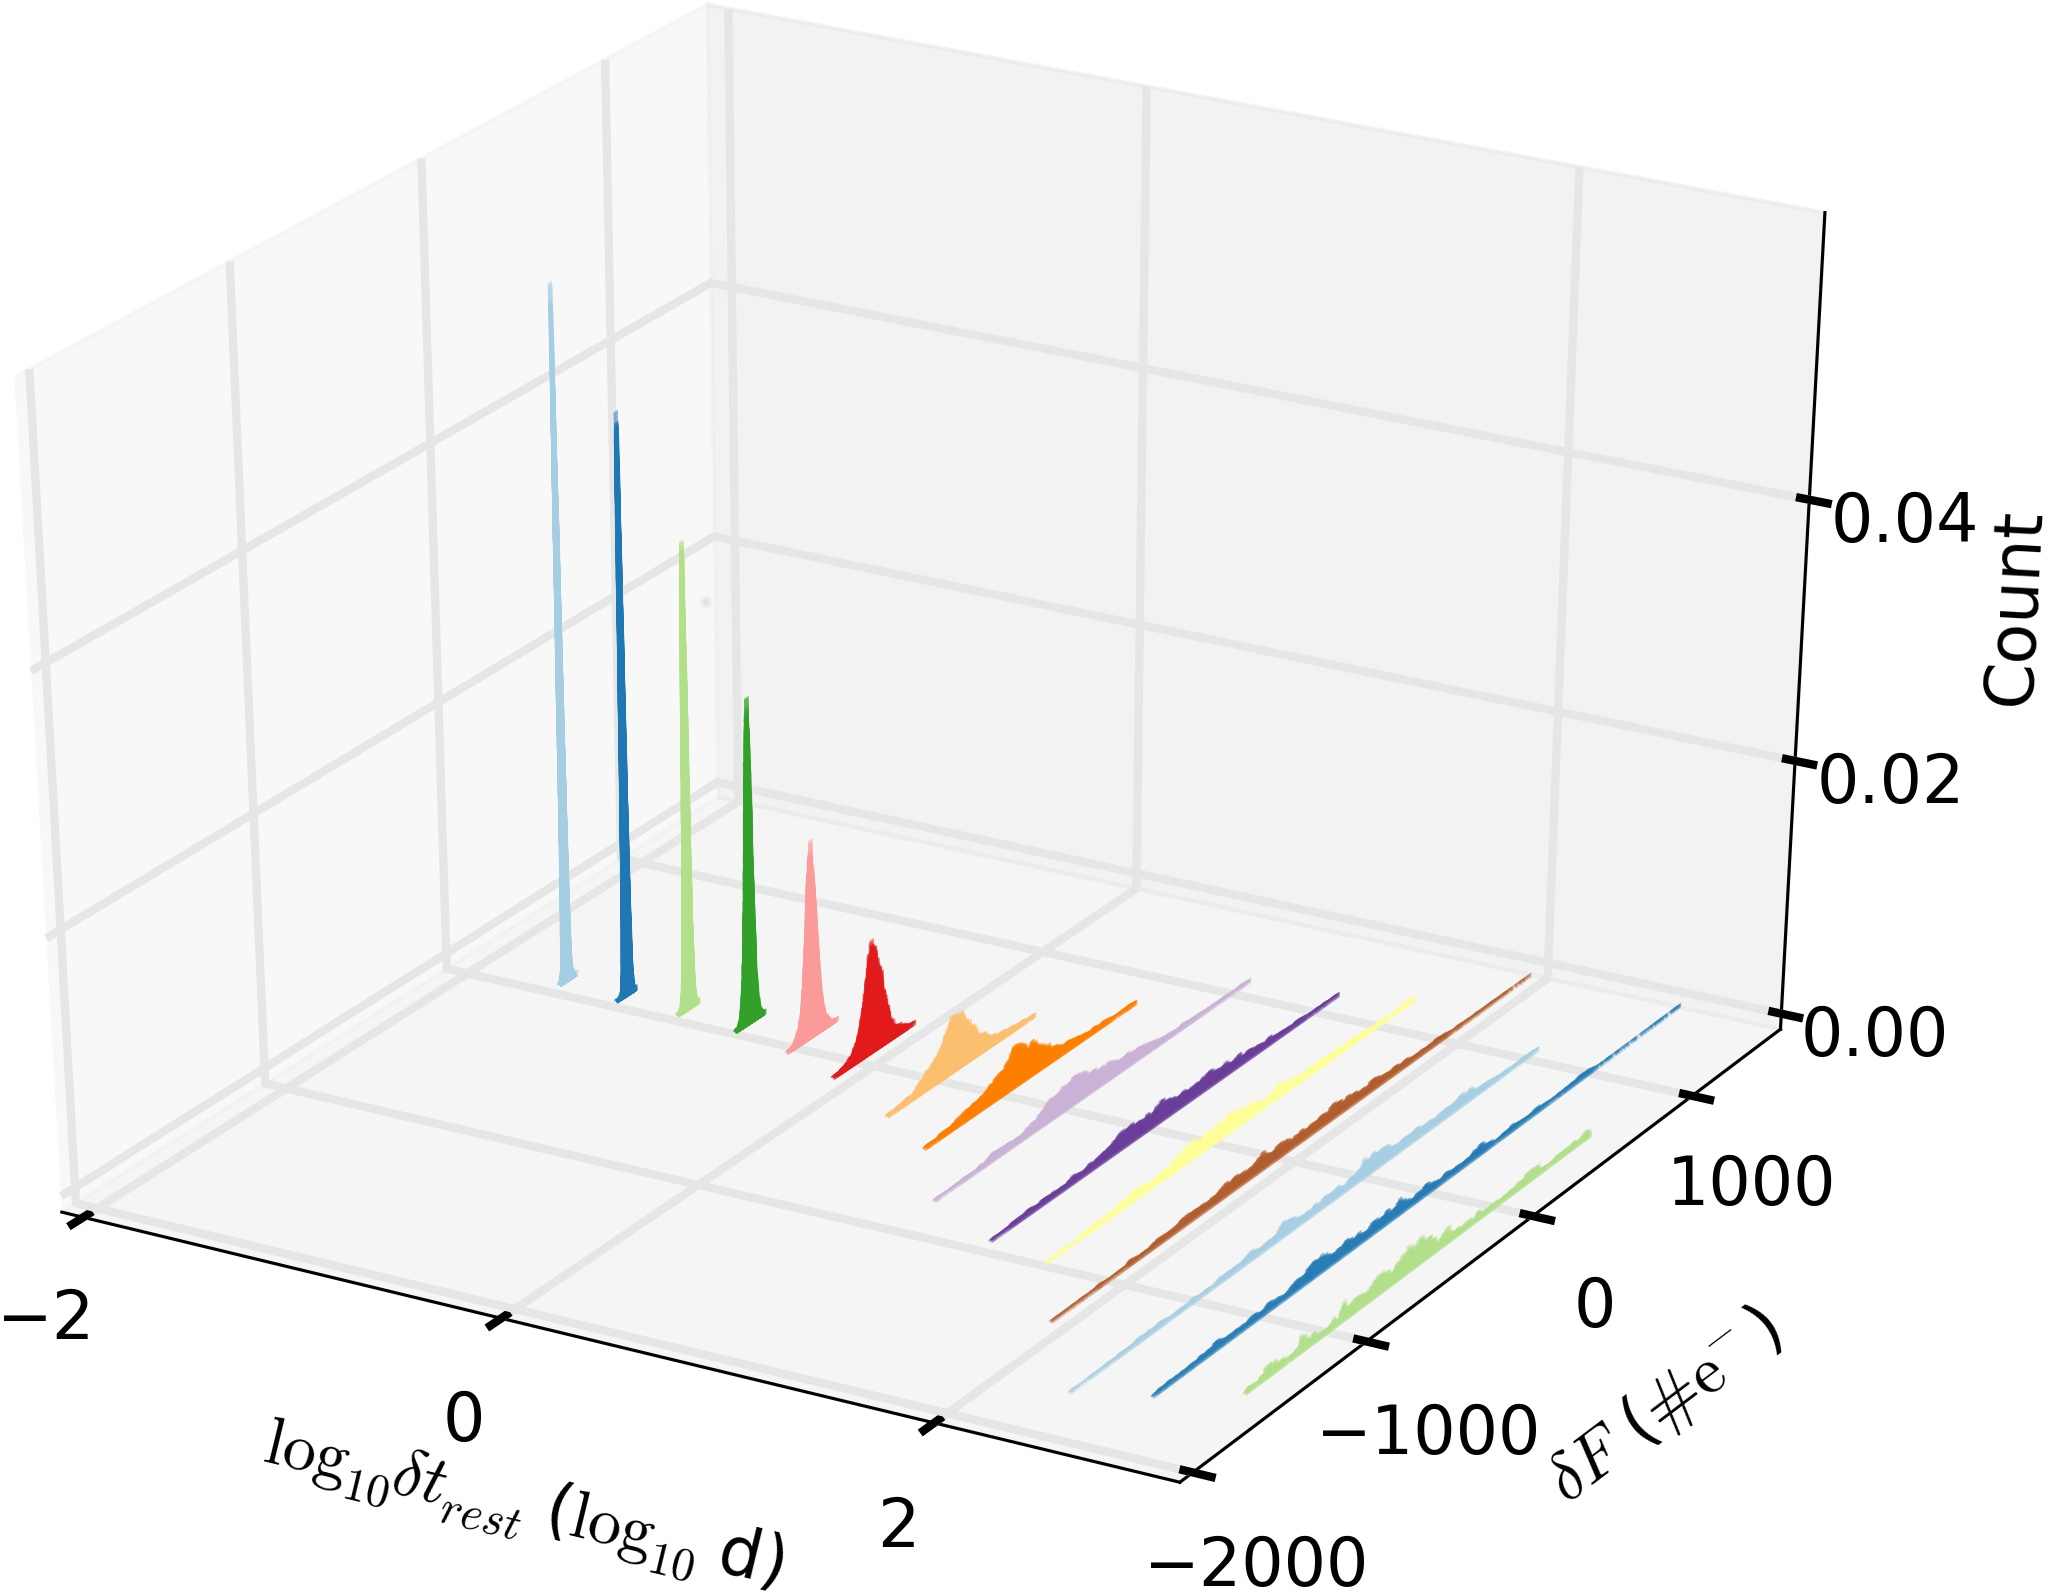
\includegraphics[scale=0.0875]{images/kplr006932990-1stIncr_3D.jpg}
      \end{figure}
      \centering
      {\tiny How does variance of $\delta F$ vary with $\delta t$?}
    \end{column}
    \begin{column}{0.4\textwidth}
       \begin{itemize}
       %\item How to compare PSD model to data?
         %\pause
       \item $2^{\mathrm{nd}}$-order statistic.
       \item $\delta F = F(t+\delta t) - F(t)$
         %\pause
       \item $SF(\delta t) = \langle \vert \delta F \vert^{2} \rangle_{t}$
       %\item How does variance of $\delta F$ vary with $\delta t$.
         %\pause
       \item Insensitive to edge-effects, aliasing etc...
       %\item Spurious breaks \& features may occur - must be careful! {\tiny \citep{emm10}}
       \item $SF(\delta t) = 2ACVF(0) - 2ACVF(\delta t)$
       \end{itemize}
    \end{column}
  \end{columns}
\end{frame}

\begin{frame}
\frametitle{Structure functions}
  \begin{columns}
    \centering
    \begin{column}{0.55\textwidth}
      \begin{figure}
        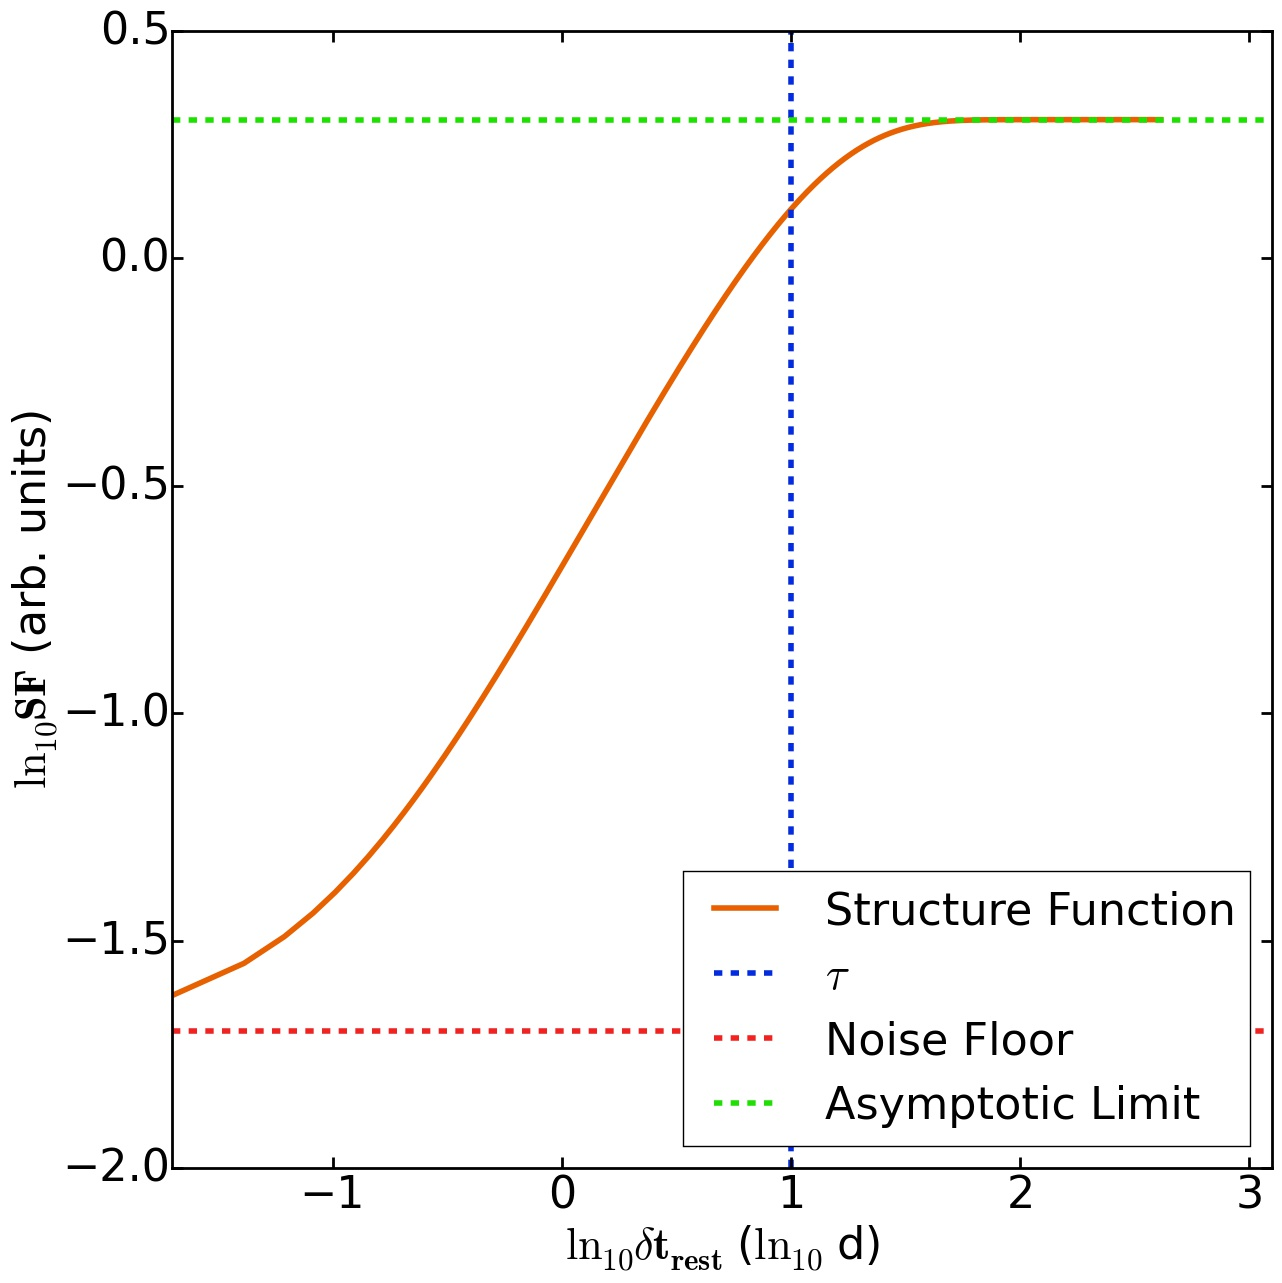
\includegraphics[scale=0.12]{images/SF_Illustration.jpg}
      \end{figure}
      \centering
      {\tiny Features in the Structure Function}
    \end{column}
    \begin{column}{0.45\textwidth}
       \begin{itemize}
       %\item How to compare PSD model to data?
         %\pause
       \item Small $\delta t$: `Noise floor'
       \item Slope $\sim \gamma$
         %\pause
       \item Big $\delta t$: Turnover i.e. damping
       %\item How does variance of $\delta F$ vary with $\delta t$.
         %\pause
       %\item Insensitive to edge-effects, aliasing etc...
       \item Spurious breaks \& features {\tiny \citep{Emm10}}
       \end{itemize}
    \end{column}
  \end{columns}
\end{frame}

\subsection{Kepler Systematics}

\begin{frame}
\frametitle{Are the MAST light curves accurate?}
  \begin{columns}
    \begin{column}{0.5\textwidth}
      \begin{figure}
        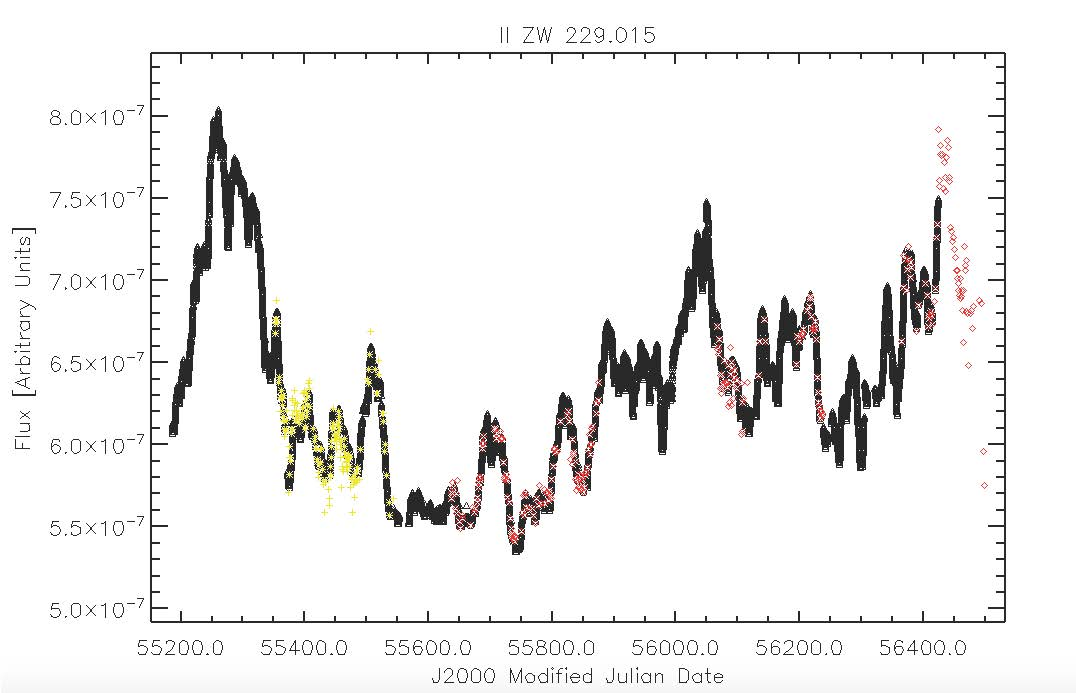
\includegraphics[scale=0.1525]{images/p2fig1.jpg}
      \end{figure}
      \begin{center}
        {\tiny \citet*{CariniWilliamsAAS}}
      \end{center}
    \begin{itemize}
      \item Spacecraft induced systematics
    \end{itemize}
    \end{column}
    \begin{column}{0.5\textwidth}
      \begin{figure}
        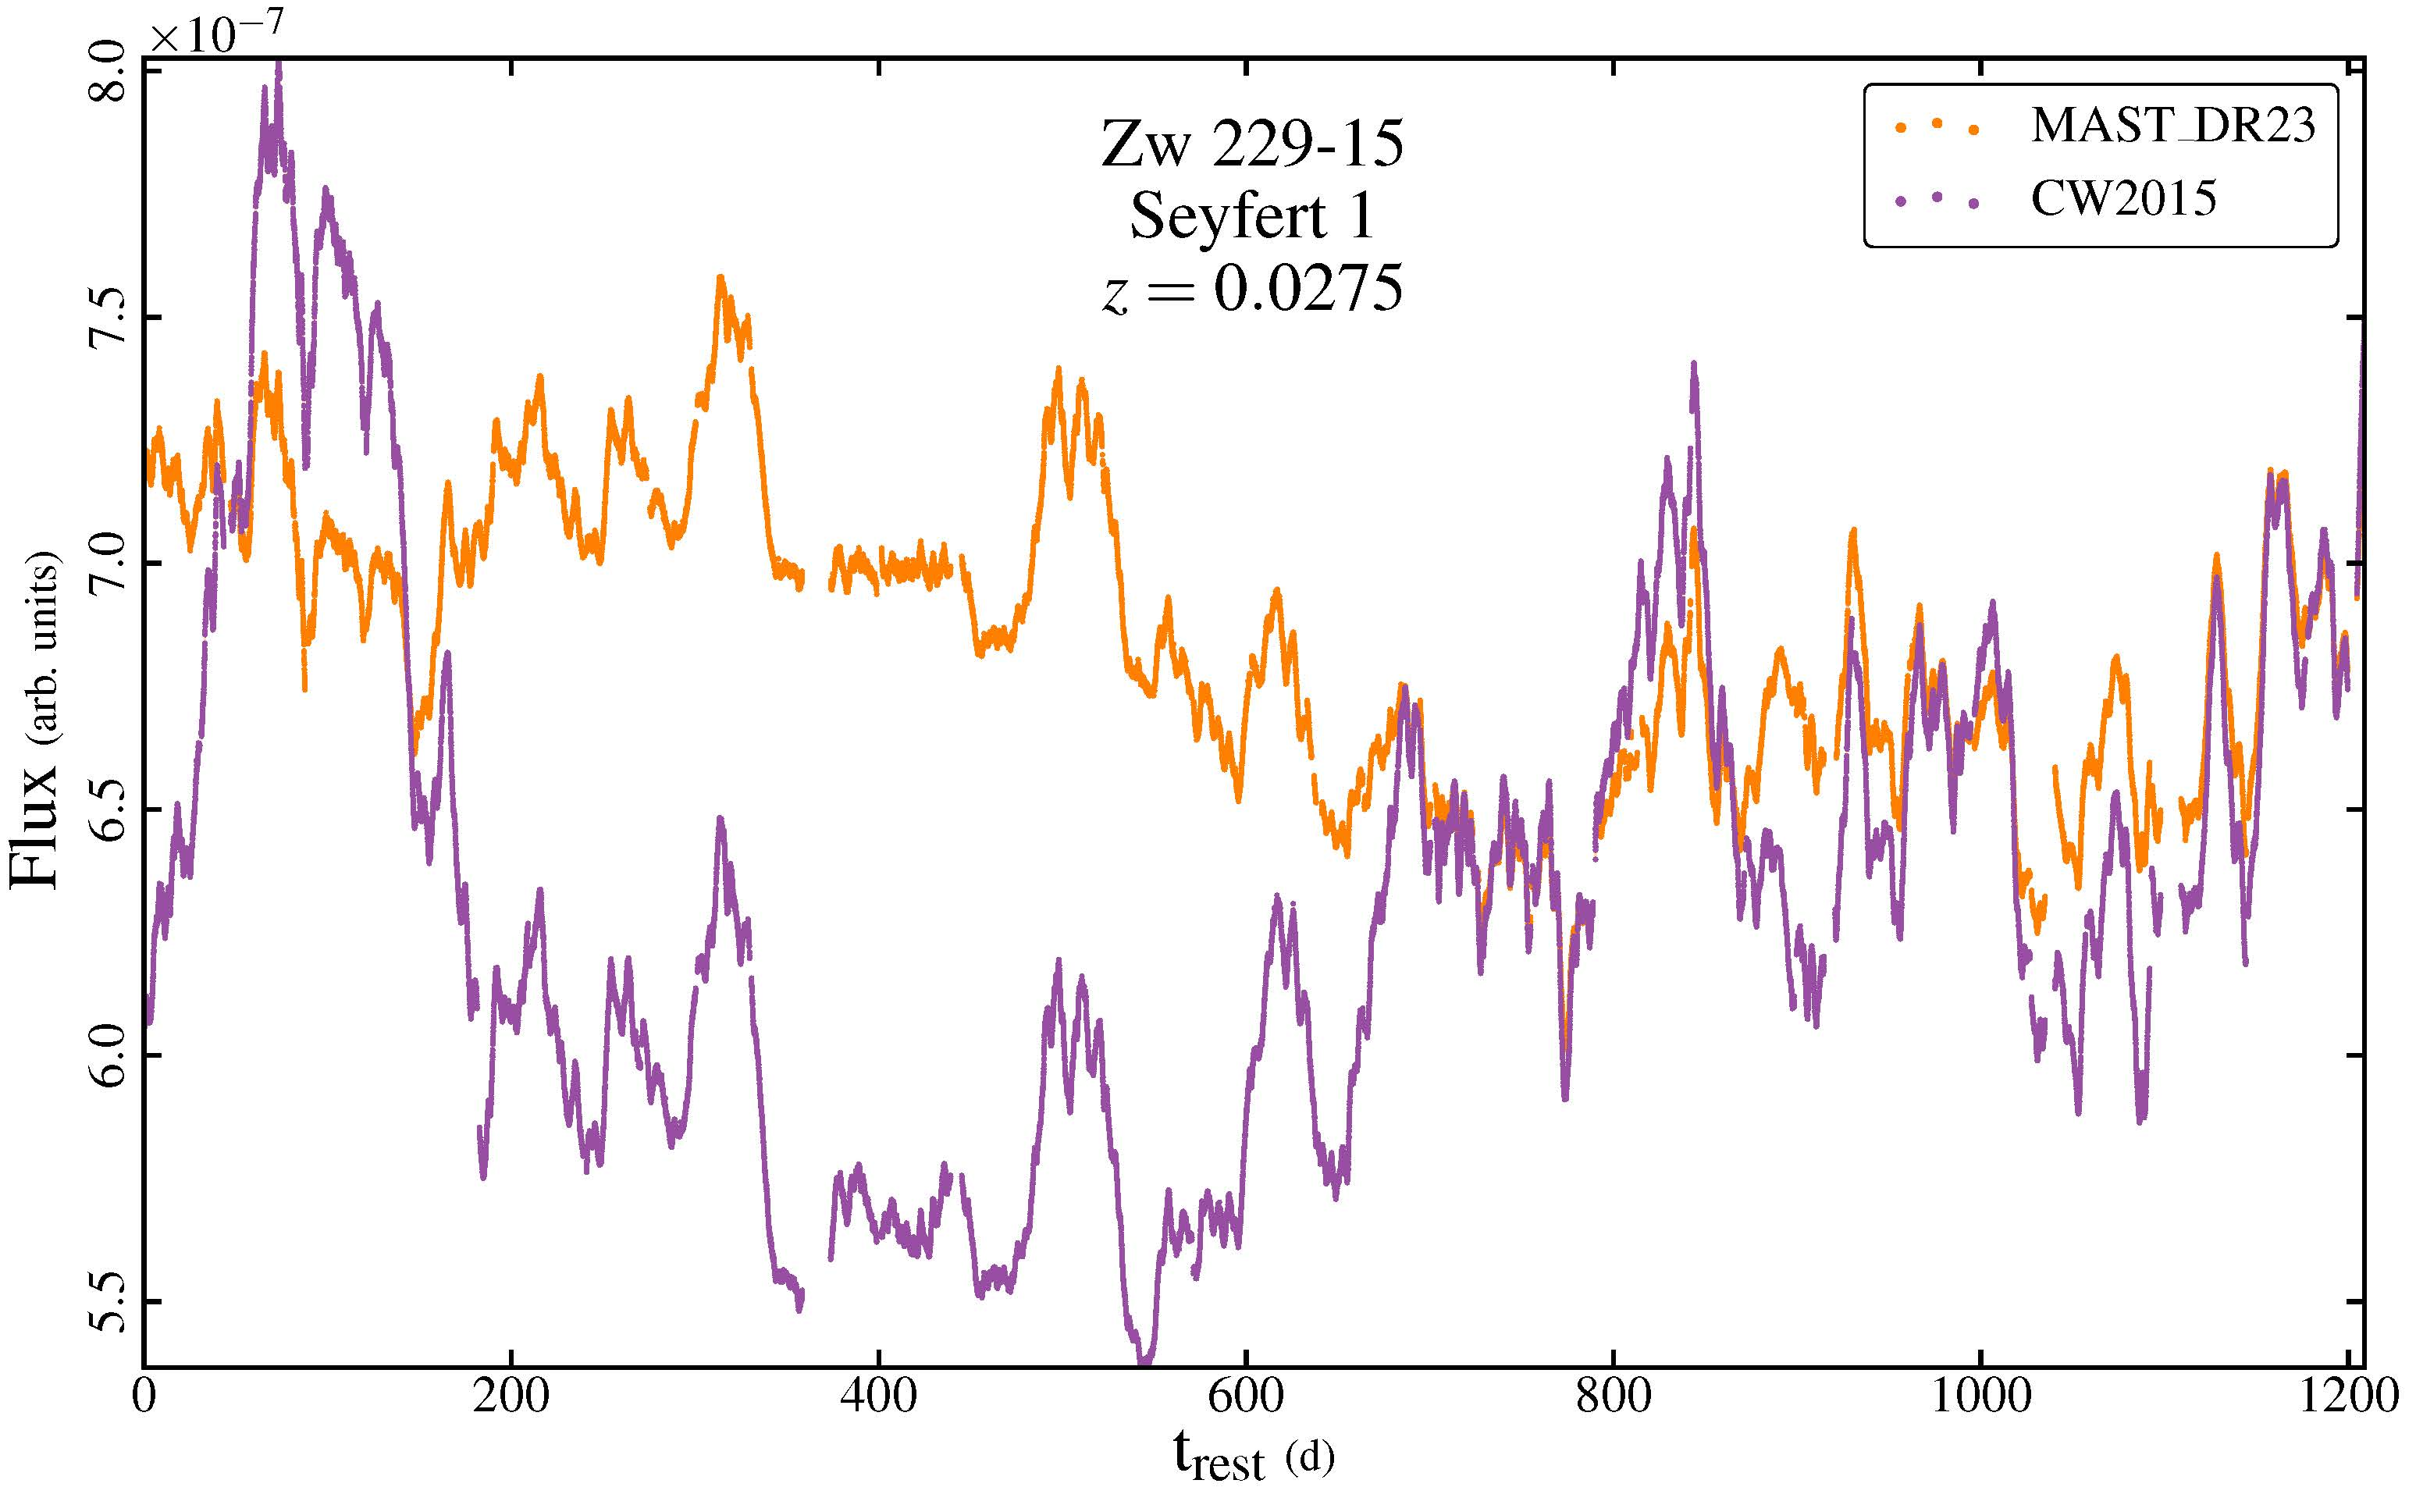
\includegraphics[scale=0.13]{images/p2fig2.jpg}
      \end{figure}
    \begin{itemize}
      \item Incorrect photometric aperture
    \end{itemize}
    \end{column}
  \end{columns}
\end{frame}

\begin{frame}
\frametitle{Photometric aperture definition \& de-trending}
  \begin{figure}
    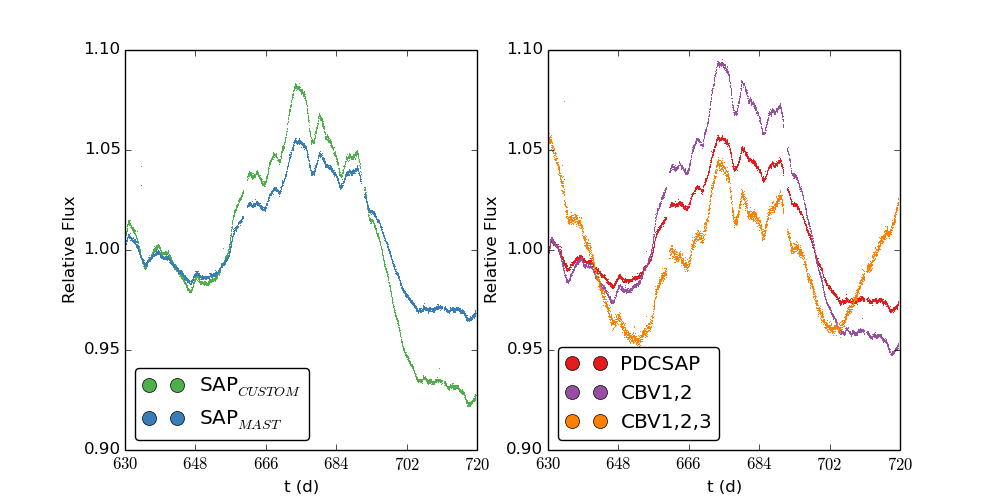
\includegraphics[scale=0.35]{images/kplr006932990-Q7_LCs.jpg}
  \end{figure}
  \begin{center}
    \href{http://www.drexel.edu/physics/contact/graduate/Moreno\ Jackeline/}{{\tiny Jackeline Moreno}}
  \end{center}
  \begin{center}
    \centering
    \begin{itemize}
      \item Flux re-extraction possible
      \item De-trending can be re-done
    \end{itemize}
  \end{center}
\end{frame}

\begin{frame}
\frametitle{Effect on Structure Functions Analysis}
  \begin{columns}
    \begin{column}{0.65\textwidth}
      \begin{figure}
        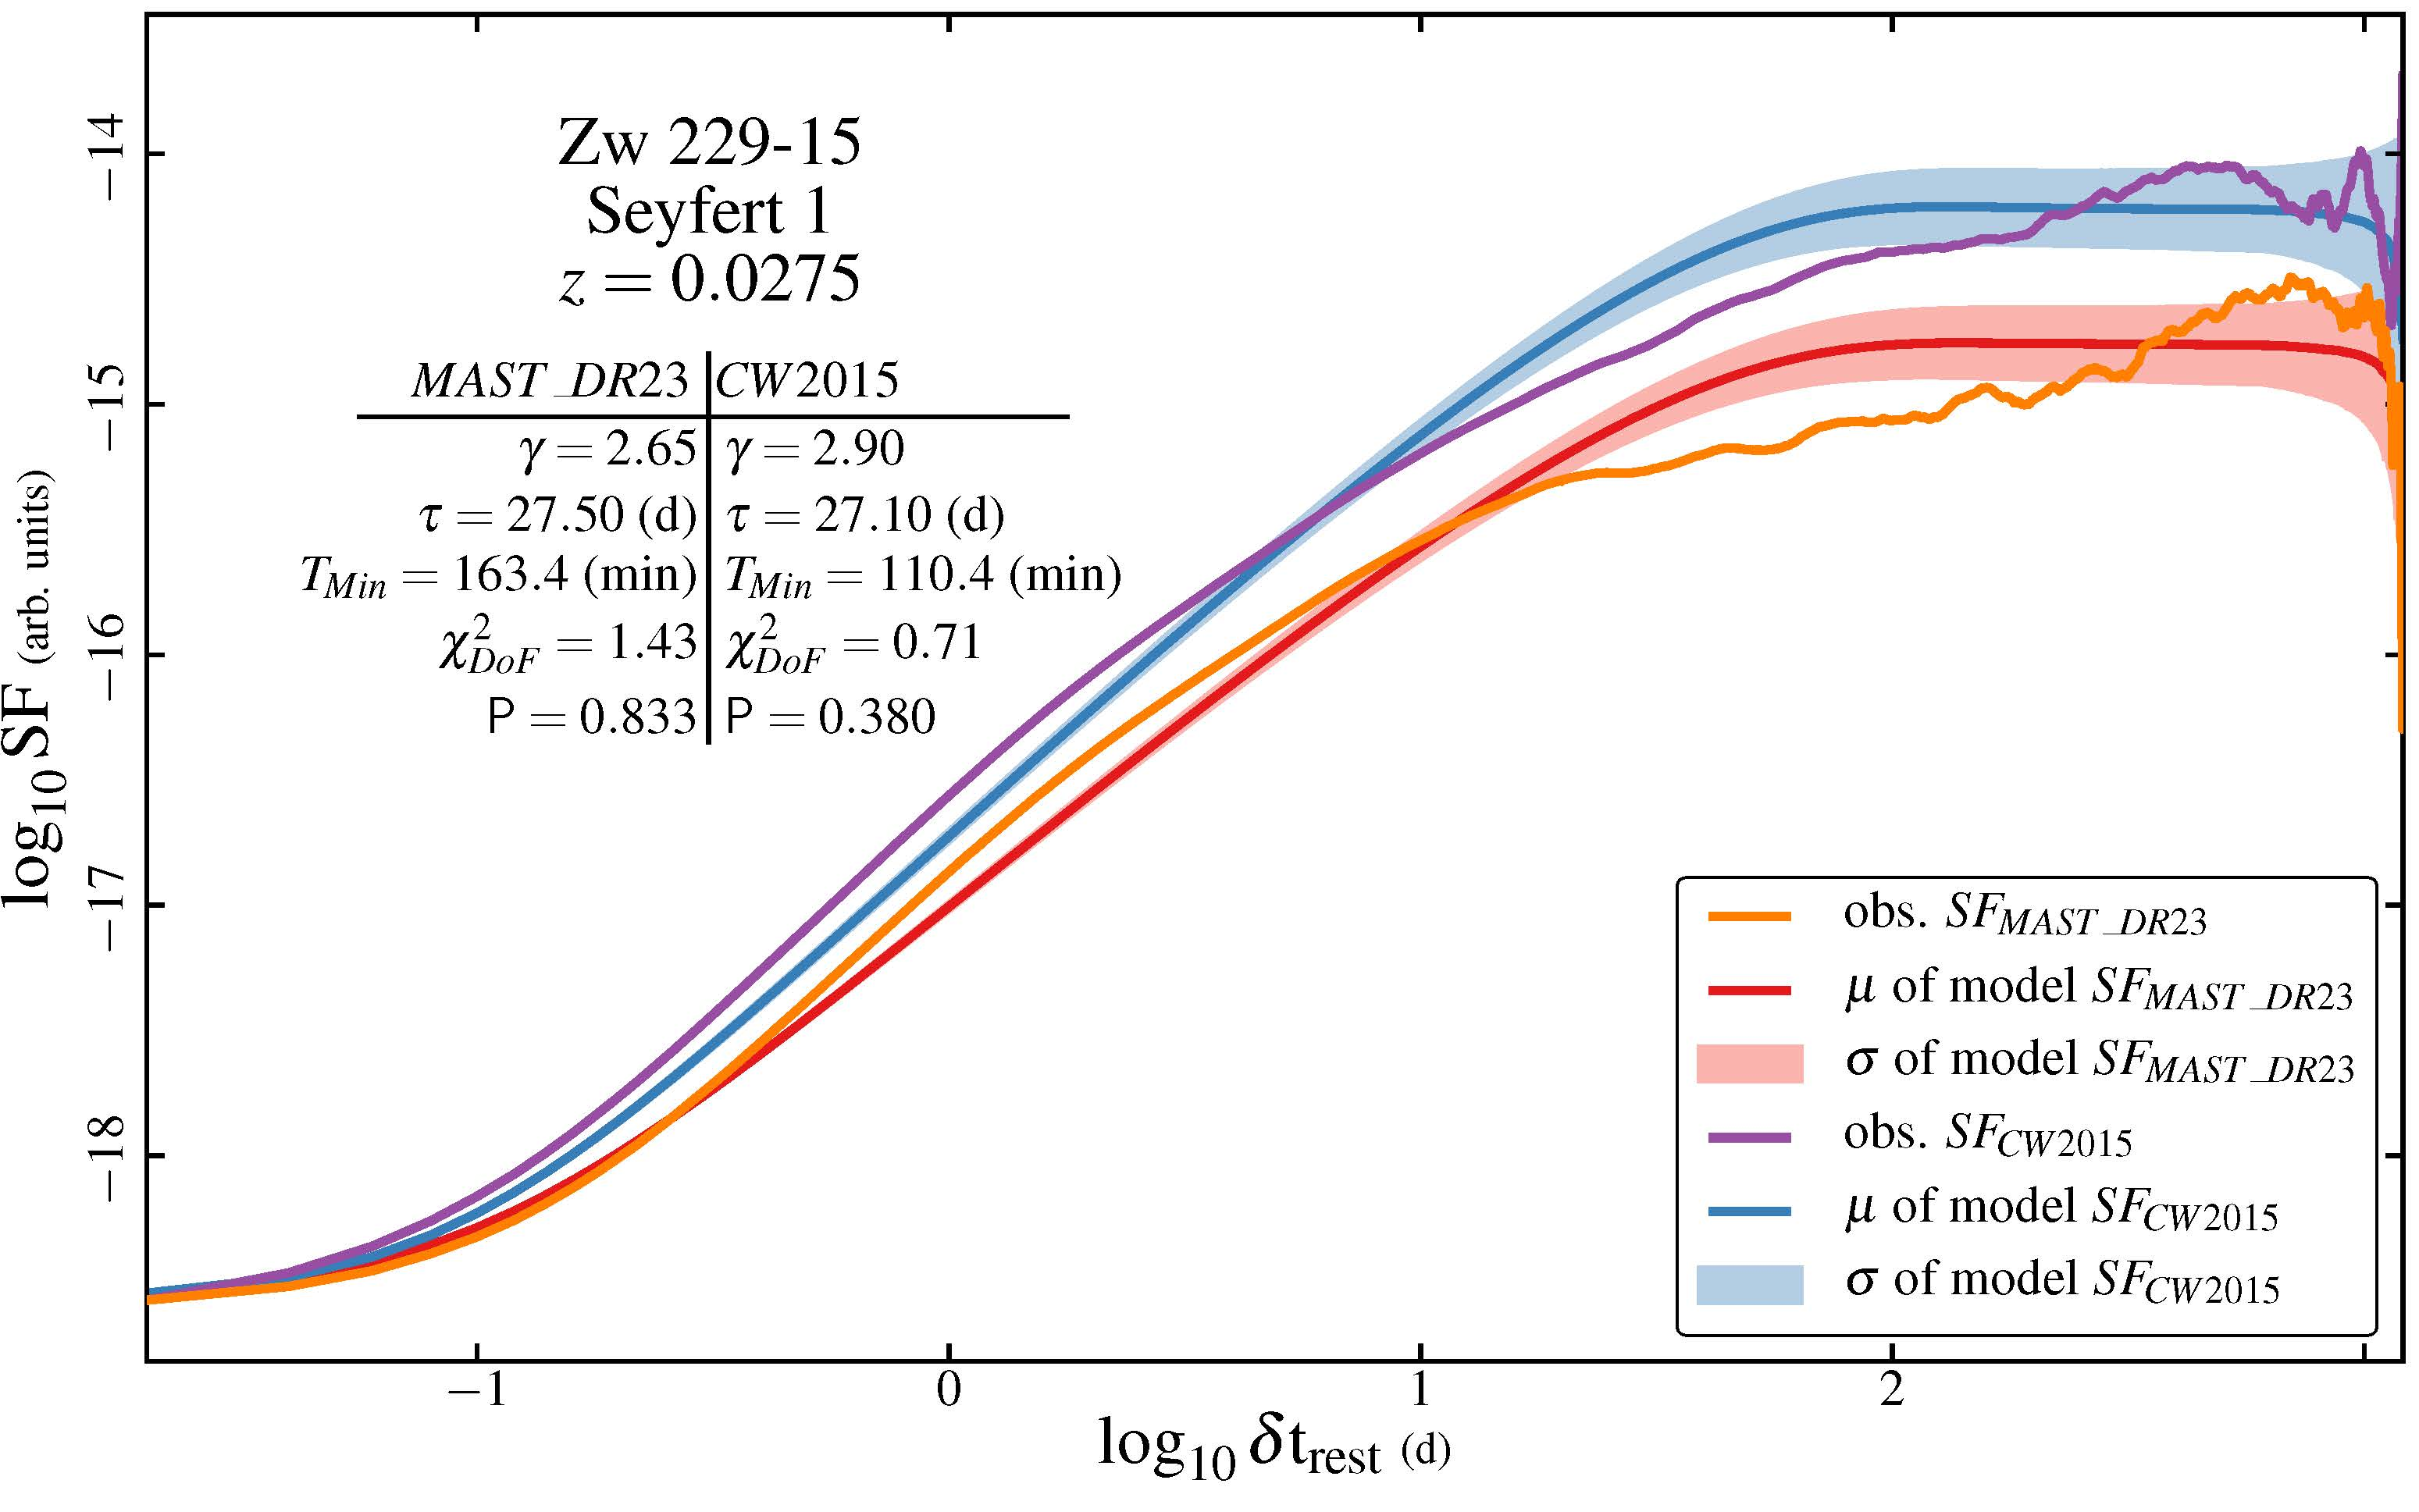
\includegraphics[scale=0.2]{images/p2fig3.jpg}
      \end{figure}
    \end{column}
    \begin{column}{0.35\textwidth}
      \begin{itemize}
        \item Instrumentation not responsible for non-DRW behavior
        \item Ground-based supplementary data crucial
      \end{itemize}
      %\begin{figure}
        %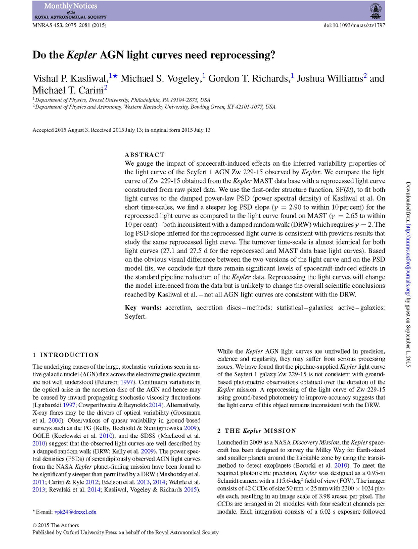
\includegraphics[scale=0.3]{images/MNRAS-2015-Kasliwal-2075-81_small.jpg}
      %\end{figure}
      {\tiny \citet{Kasliwal15b}}
    \end{column}
  \end{columns}
\end{frame}

\begin{frame}
\frametitle{Structure function fits}
  \begin{columns}
    \centering
    \begin{column}{0.65\textwidth}
      \begin{figure}
        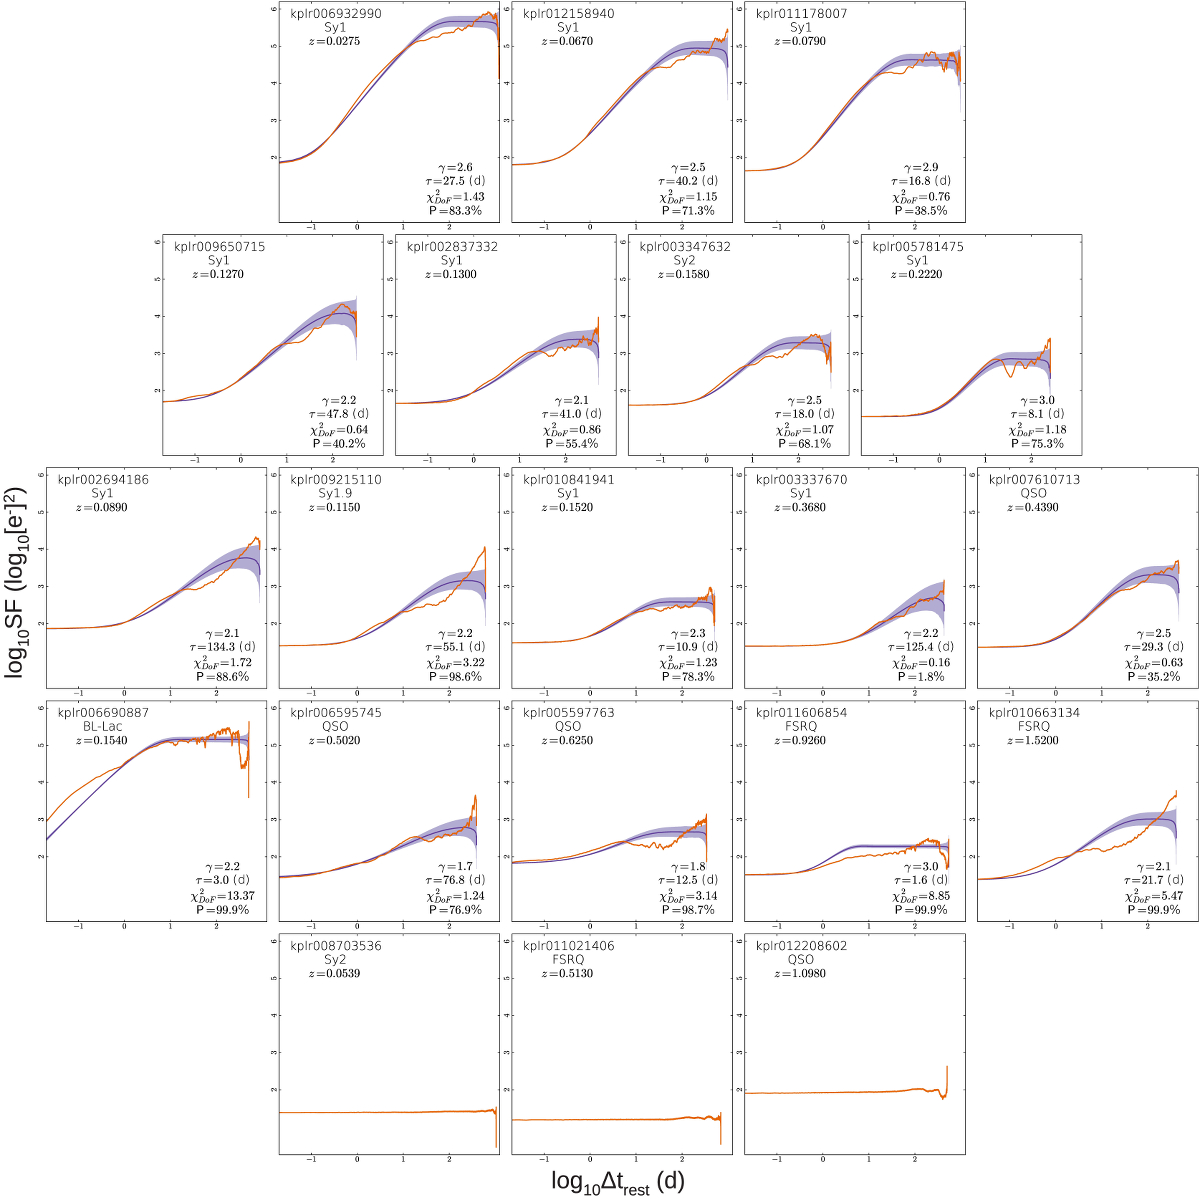
\includegraphics[scale=0.45]{images/AllSF.jpg}
      \end{figure}
    \end{column}
    \begin{column}{0.35\textwidth}
        \begin{itemize}
        \item Not all AGN $\sim$ DRW
        \item PSD model too simple
        \item Variability onsets over $\sim 1$~hr to $\sim 1$~d
        %\item \cite{Kasliwal15}
        %\item Can't be due to 'stitching' or PDC corrections.
        \end{itemize}
        %\begin{figure}
          %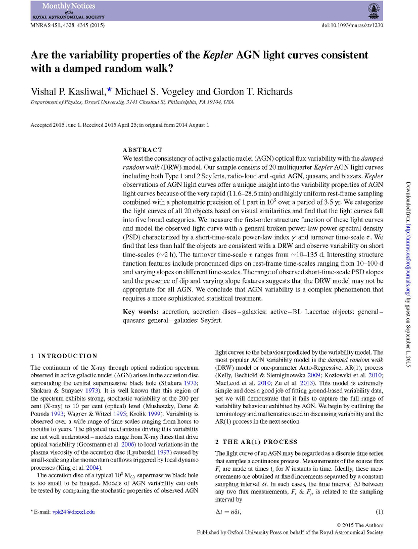
\includegraphics[scale=0.3]{../images/talk/MNRAS-2015-Kasliwal-4328-45_small.jpg}
        %\end{figure}
          {\tiny \citet*{Kasliwal15}}
    \end{column}
  \end{columns}
\end{frame}

\section{Exact MLE}

\subsection{Generalized Stochastic Processes}

\begin{frame}
\frametitle{Periodogram of Zw 229-15\\What model to use?}
  \begin{figure}
    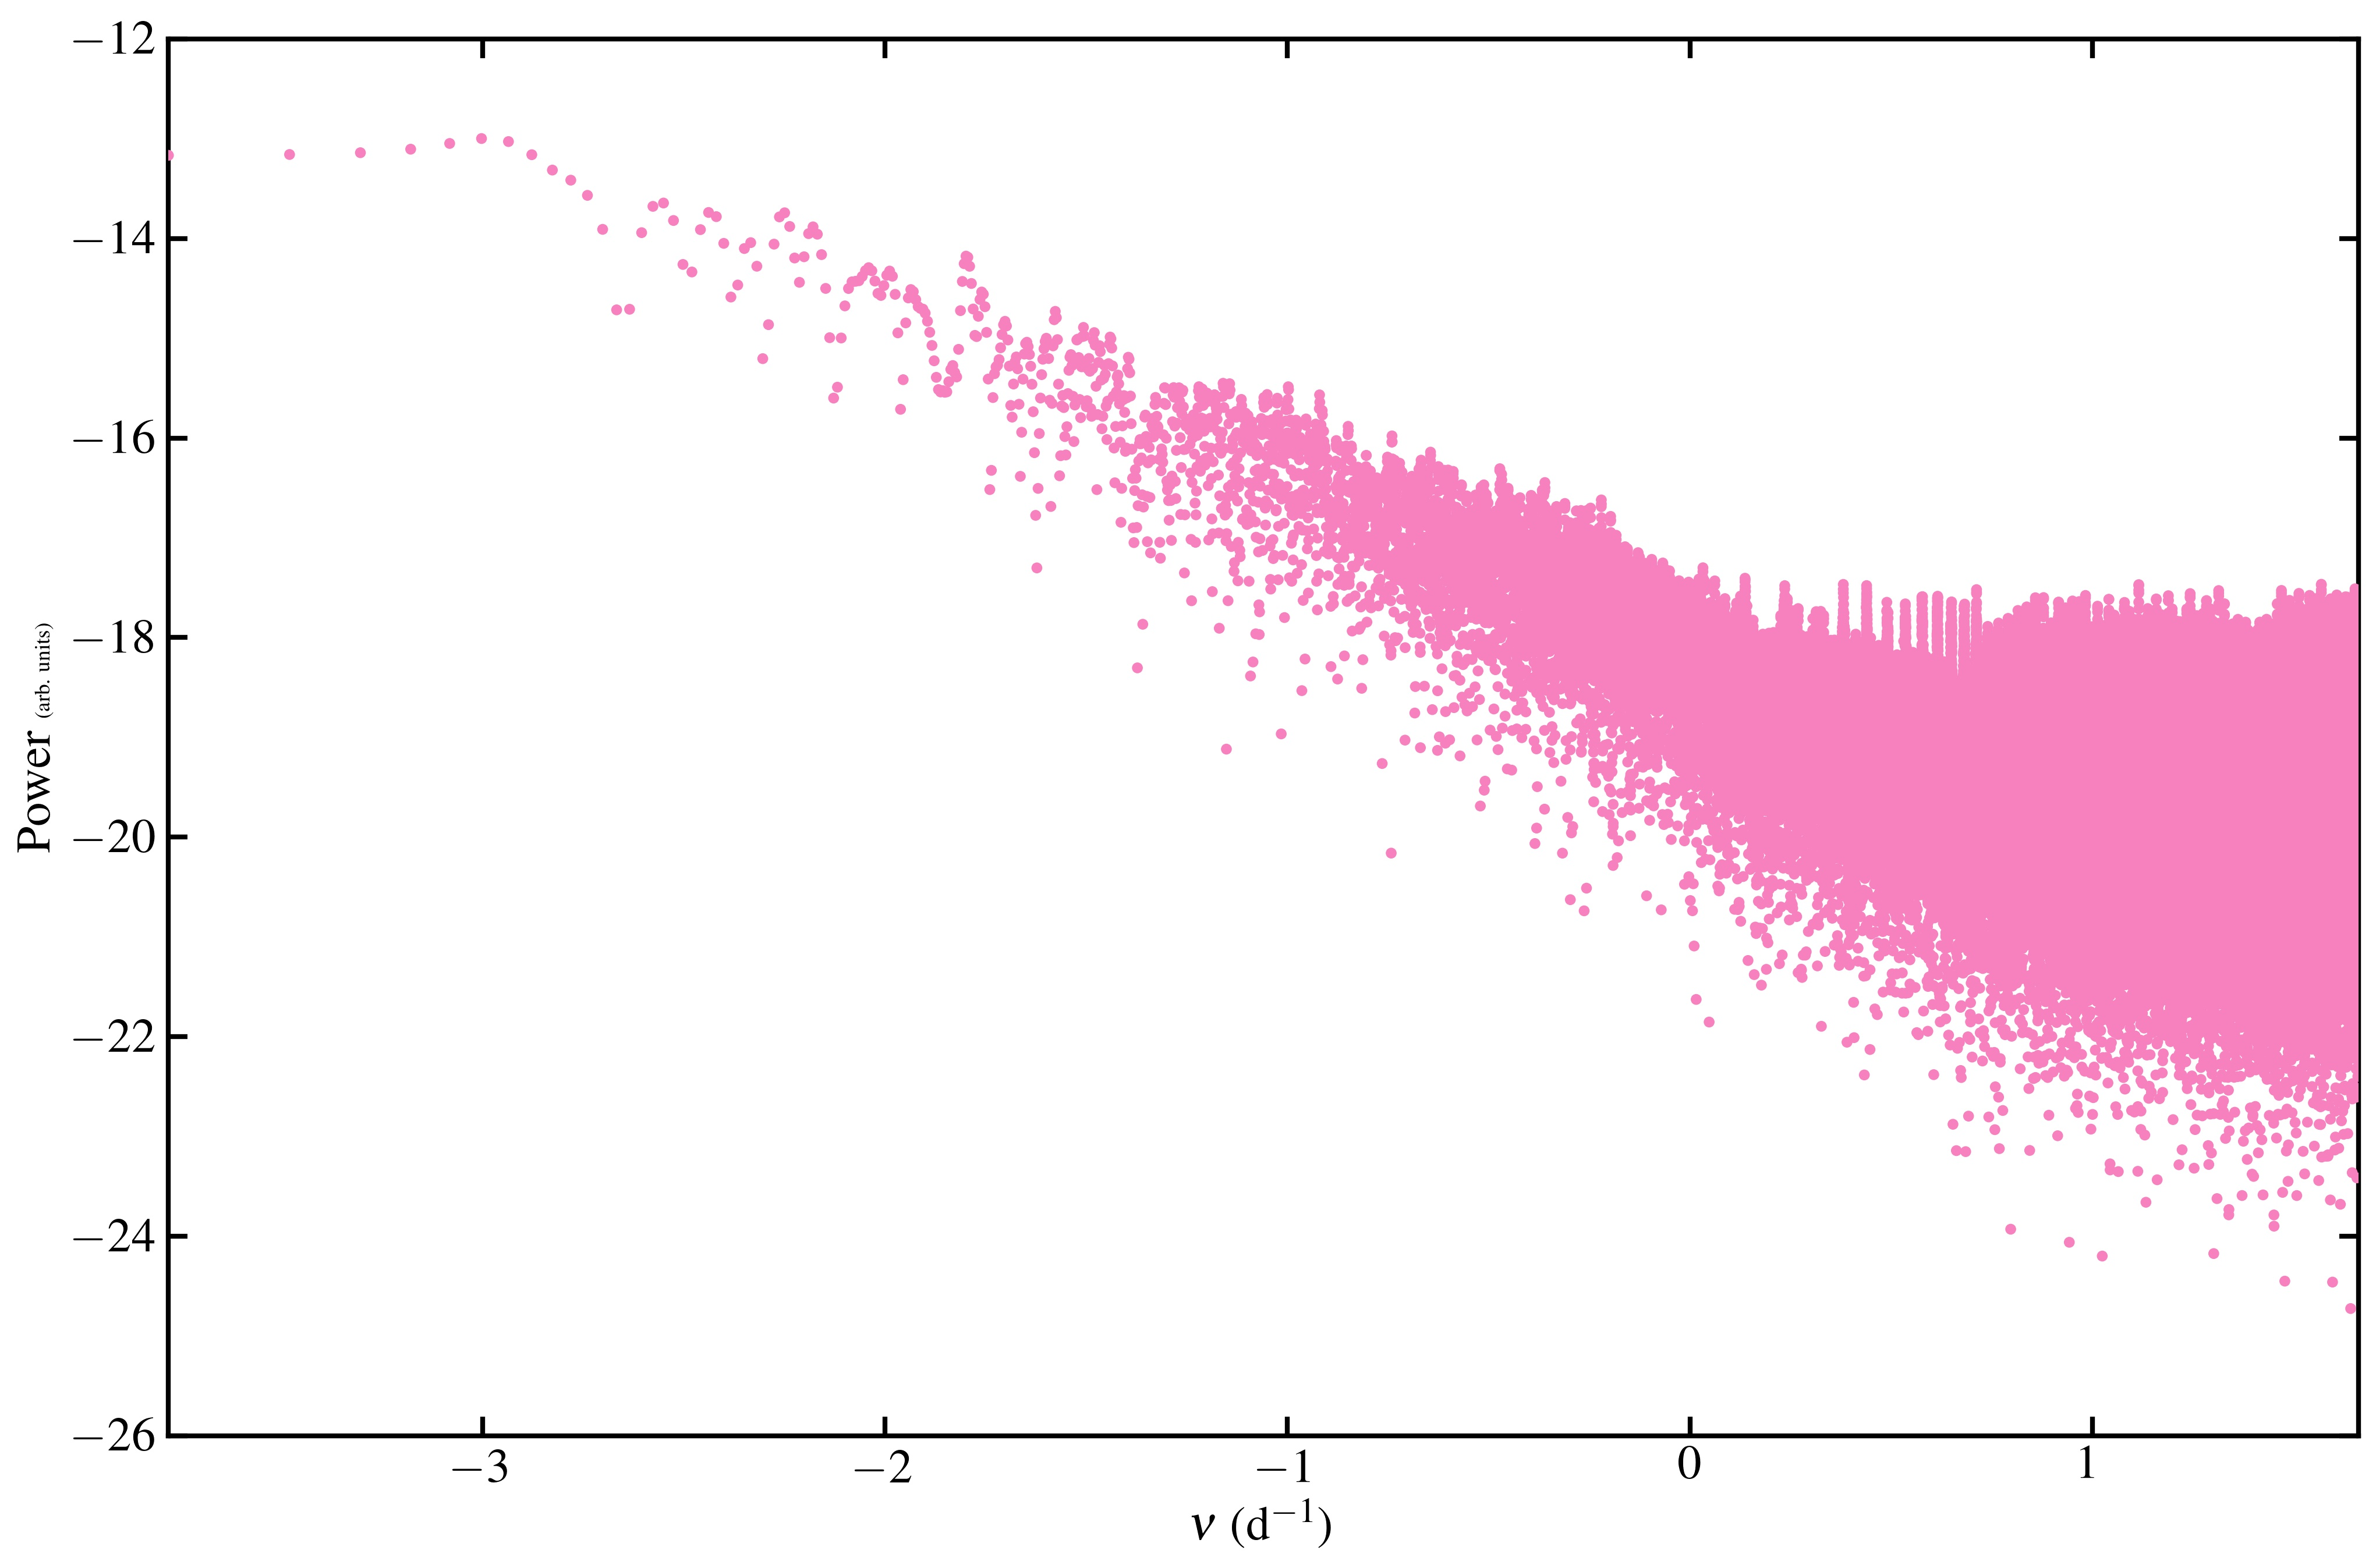
\includegraphics[scale=0.05]{images/Periodogram.jpg}
  \end{figure}
  \begin{center}
    \centering
    \begin{itemize}
      \item Stochastic model must be flexible
      \item Amenable to physical interpretation
    \end{itemize}
  \end{center}
\end{frame}

\begin{frame}
\frametitle{Random Walks}
  \begin{columns}
    \centering
    \begin{column}{0.5\textwidth}
      \begin{figure}
        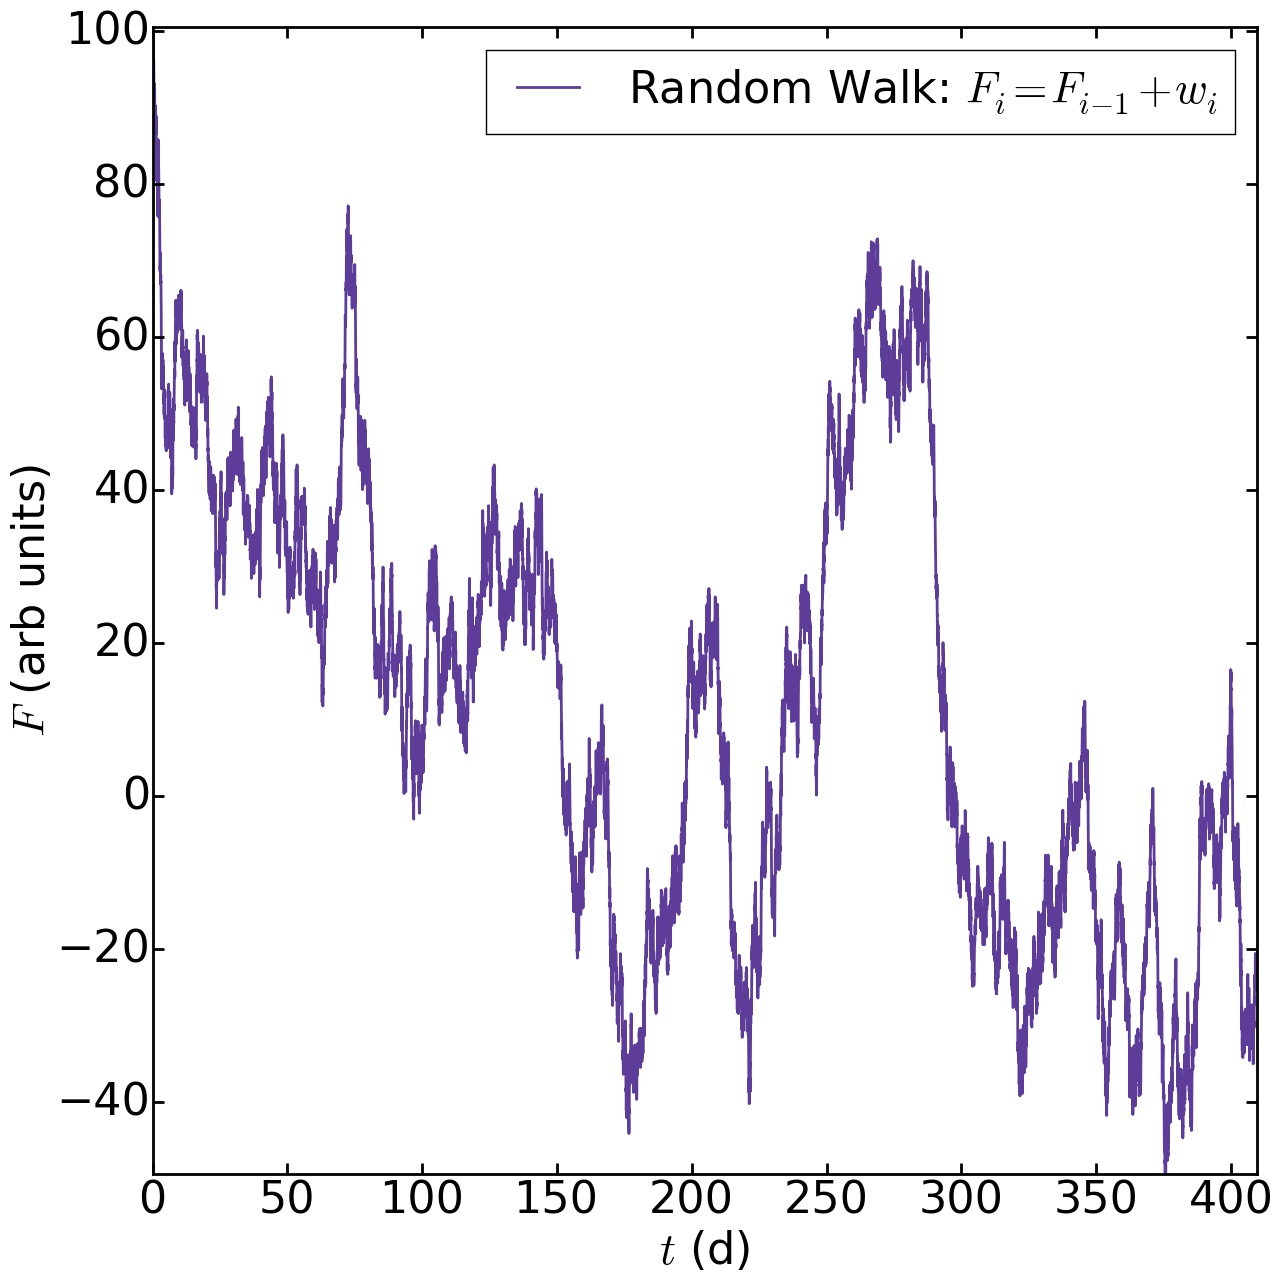
\includegraphics[scale=0.12]{images/RW_Illustration.jpg}
      \end{figure}
      \centering
      %{\tiny $\tau = 1$ d.}
    \end{column}
    \begin{column}{0.5\textwidth}
    \begin{itemize}
      \item Accretion disk: MHD `Hot-spots'
      \item Random `disturbances'
        \begin{itemize}
          \item $w_{i} \sim \mathcal{N}(0,\sigma^{2})$
        \end{itemize}
      \item $F_{i+1} = F_{i} + w_{i}$
      \item Not stationary - flux `walks away'
    \end{itemize}
    \end{column}
  \end{columns}
\end{frame}

\begin{frame}
\frametitle{The Damped Random Walk}
  \begin{columns}
    \centering
    \begin{column}{0.5\textwidth}
      \begin{figure}
        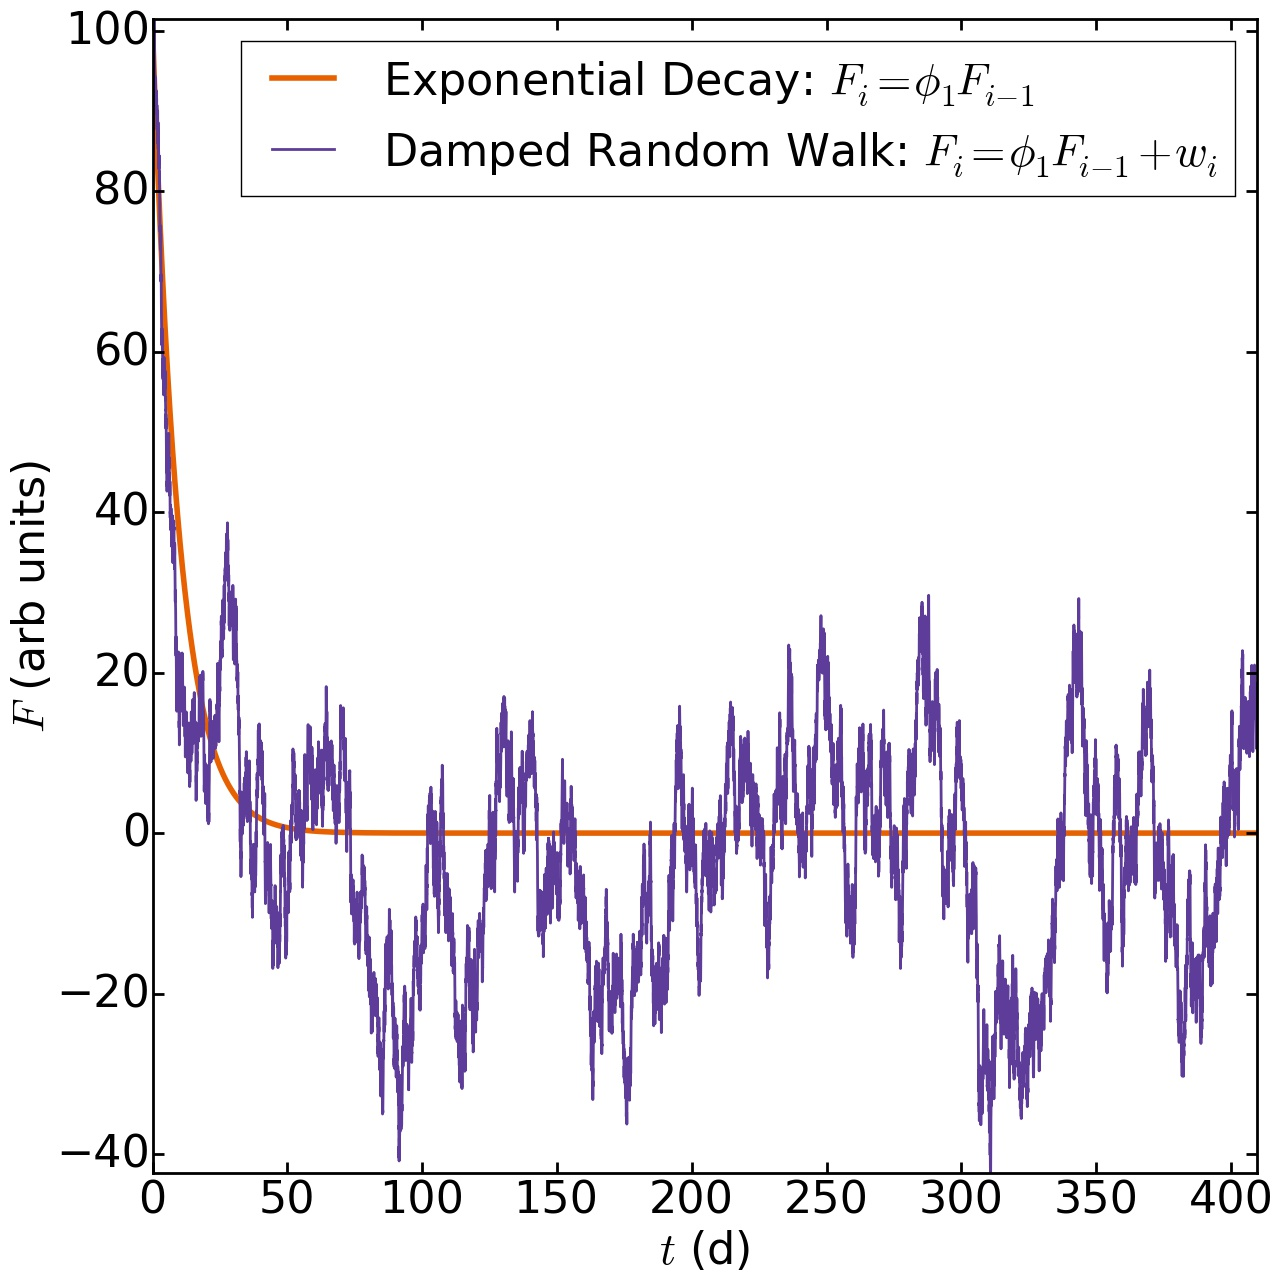
\includegraphics[scale=0.12]{images/DRW_Illustration.jpg}
      \end{figure}
      \centering
      {\tiny $\tau = 1$ d.}
    \end{column}
    \begin{column}{0.5\textwidth}
    \begin{itemize}
    \item Exponential decay
      \begin{itemize}
        \item $F_{i} = \phi_{1} F_{i-1}$
        \item $\phi = e^{-\frac{\delta t}{\tau}} < 1$
        \item Decays to asymptotic flux level %{\tiny $\vert \phi \vert < 1$}
      \end{itemize}
      %\pause
    %\item Add Gaussian random number at every step.
    \item Damped Random Walk
      \begin{itemize}
        %\item $\phi = e^{-\frac{\delta t}{\tau}} < 1$.
        \item $F_{i} = \phi_{1} F_{i-1} + w_{i}$
        \item `Walks around' exponential decay%{\tiny $\vert \phi \vert < 1$ \& $w_{i} \sim \mathcal{N}(0,\sigma)$}
      \end{itemize}
    \item Exponential decay driven by Gaussian noise
    \item $1^{st}$-Order Linear Stochastic-DE
    %\item Fits OGLE and SDSS quasars \\ {\tiny \citep{kel09,koz10,mac10}}.
      %\pause
    %\item $1^{st}$-Order Linear Stochastic-DE.
    \end{itemize}
    \end{column}
  \end{columns}
\end{frame}


\end{comment}


\section{Modelling AGN Variability as a C-ARMA Process}

\subsection{Introduction}

\begin{frame}
\frametitle{Continuous-time AutoRegressive Moving Average (C-ARMA) Processes}
  \begin{equation*} \mathrm{d}W \sim \mathcal{N}(0,\mathrm{d}t) \end{equation*}
  \begin{equation*}\label{eq:CARMA} \mathrm{d}^{p}x + \alpha_{1} \mathrm{d}^{p-1}x + \ldots + \alpha_{p-1} \mathrm{d}x + \alpha_{p}x = \beta_{0} (\mathrm{d}W) + \ldots + \beta_{q} \mathrm{d}^{q}(\mathrm{d}W) \end{equation*}
  \begin{columns}
    \centering
    \begin{column}{0.5\textwidth}
      \begin{itemize}
        \item It\={o} calculus {\tiny \citet{Brockwell14,Davis,Kelly14}}
        \item Drive linearized system with noise
        \item PSD is a ratio of even polynomials in frequency
      \end{itemize}
    \end{column}
    \begin{column}{0.5\textwidth}
      \begin{figure}
        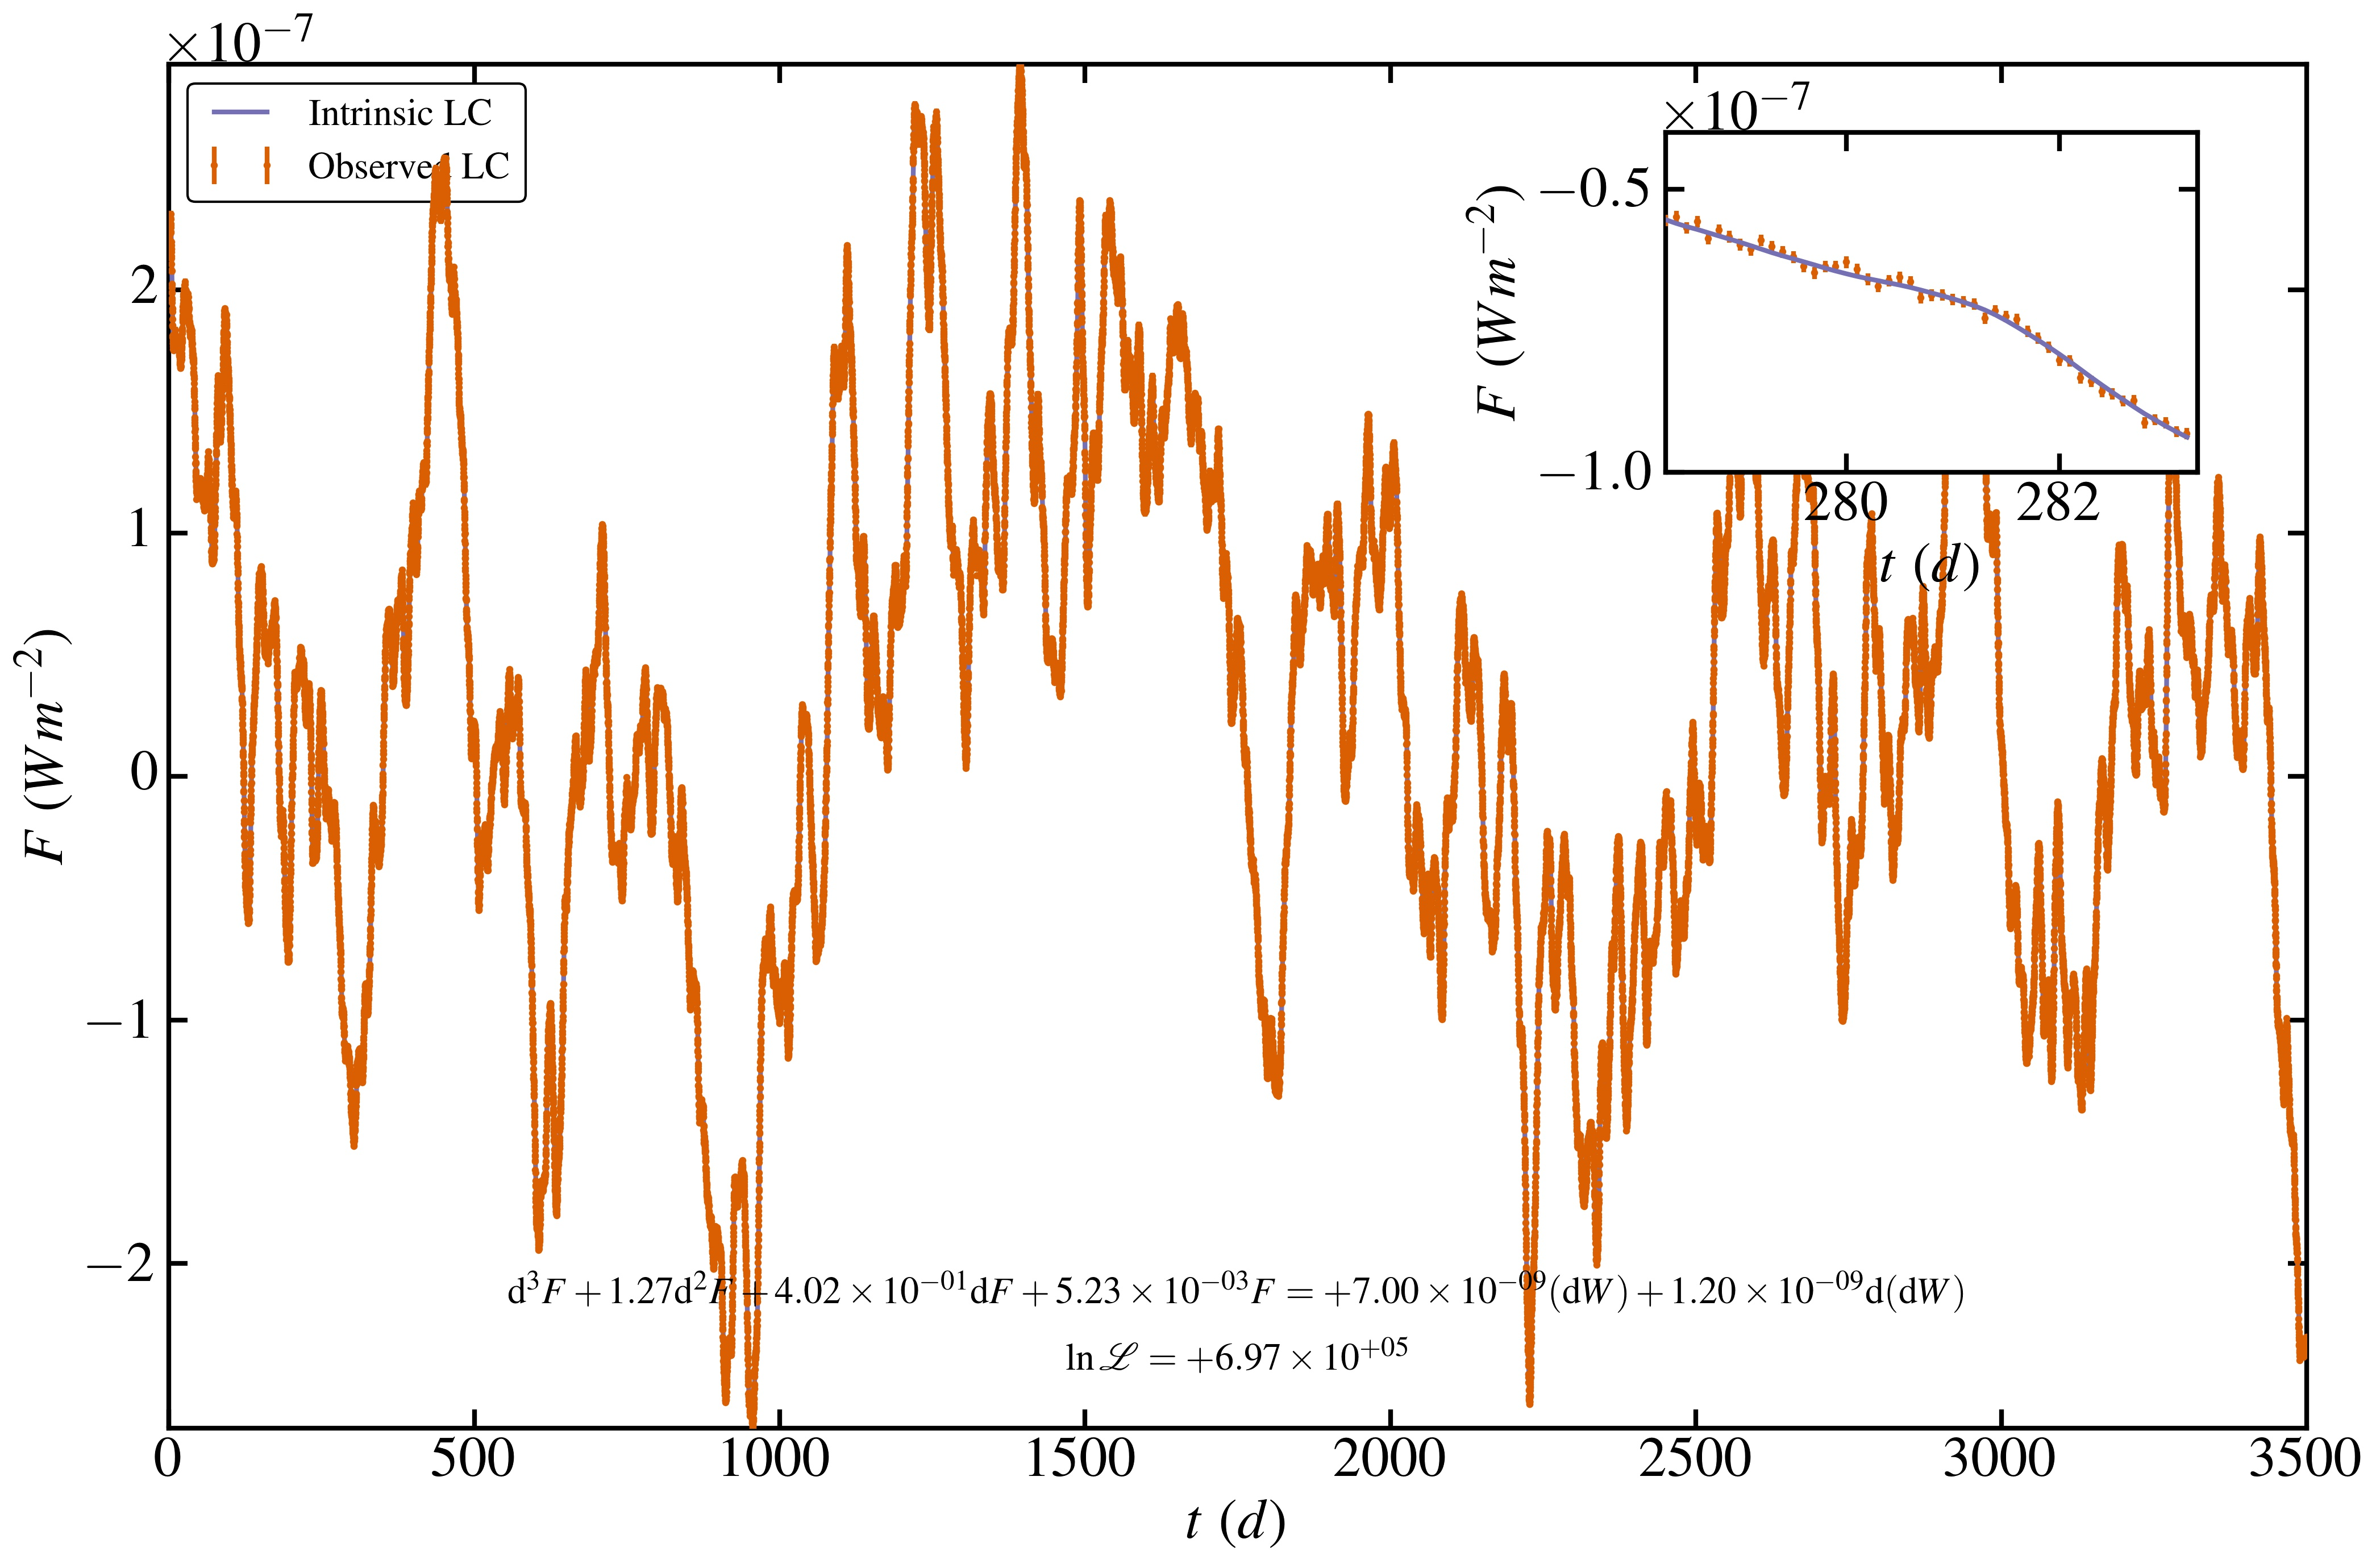
\includegraphics[scale=0.0425]{images/CARMA(3,1)_LC.jpg}
        %${\scriptstyle \mathrm{d}^{2}f + 0.7 \mathrm{d}f + 0.011f = 7.0 \times 10^{-9} (\mathrm{d}W) + 1.2 \times 10^{-9} \mathrm{d}(\mathrm{d}W)}$
      \end{figure}
    \end{column}
  \end{columns}
\end{frame}

\subsection{Why C-ARMA?}


\begin{comment}


\begin{frame}
\frametitle{Power Spectral Density\\Eg. C-ARMA($2$,$1$)}
  %\begin{equation*}\label{eq:CARMA21PSD} \mathrm{d}^{2}F + 2\omega\zeta \mathrm{d}F + \omega^{2}F = \beta_{1} \mathrm{d}(\mathrm{d}W) + \beta_{2} (\mathrm{d}W) \end{equation*}
  \begin{columns}
    \begin{column}{0.5\textwidth}
      \begin{figure}
        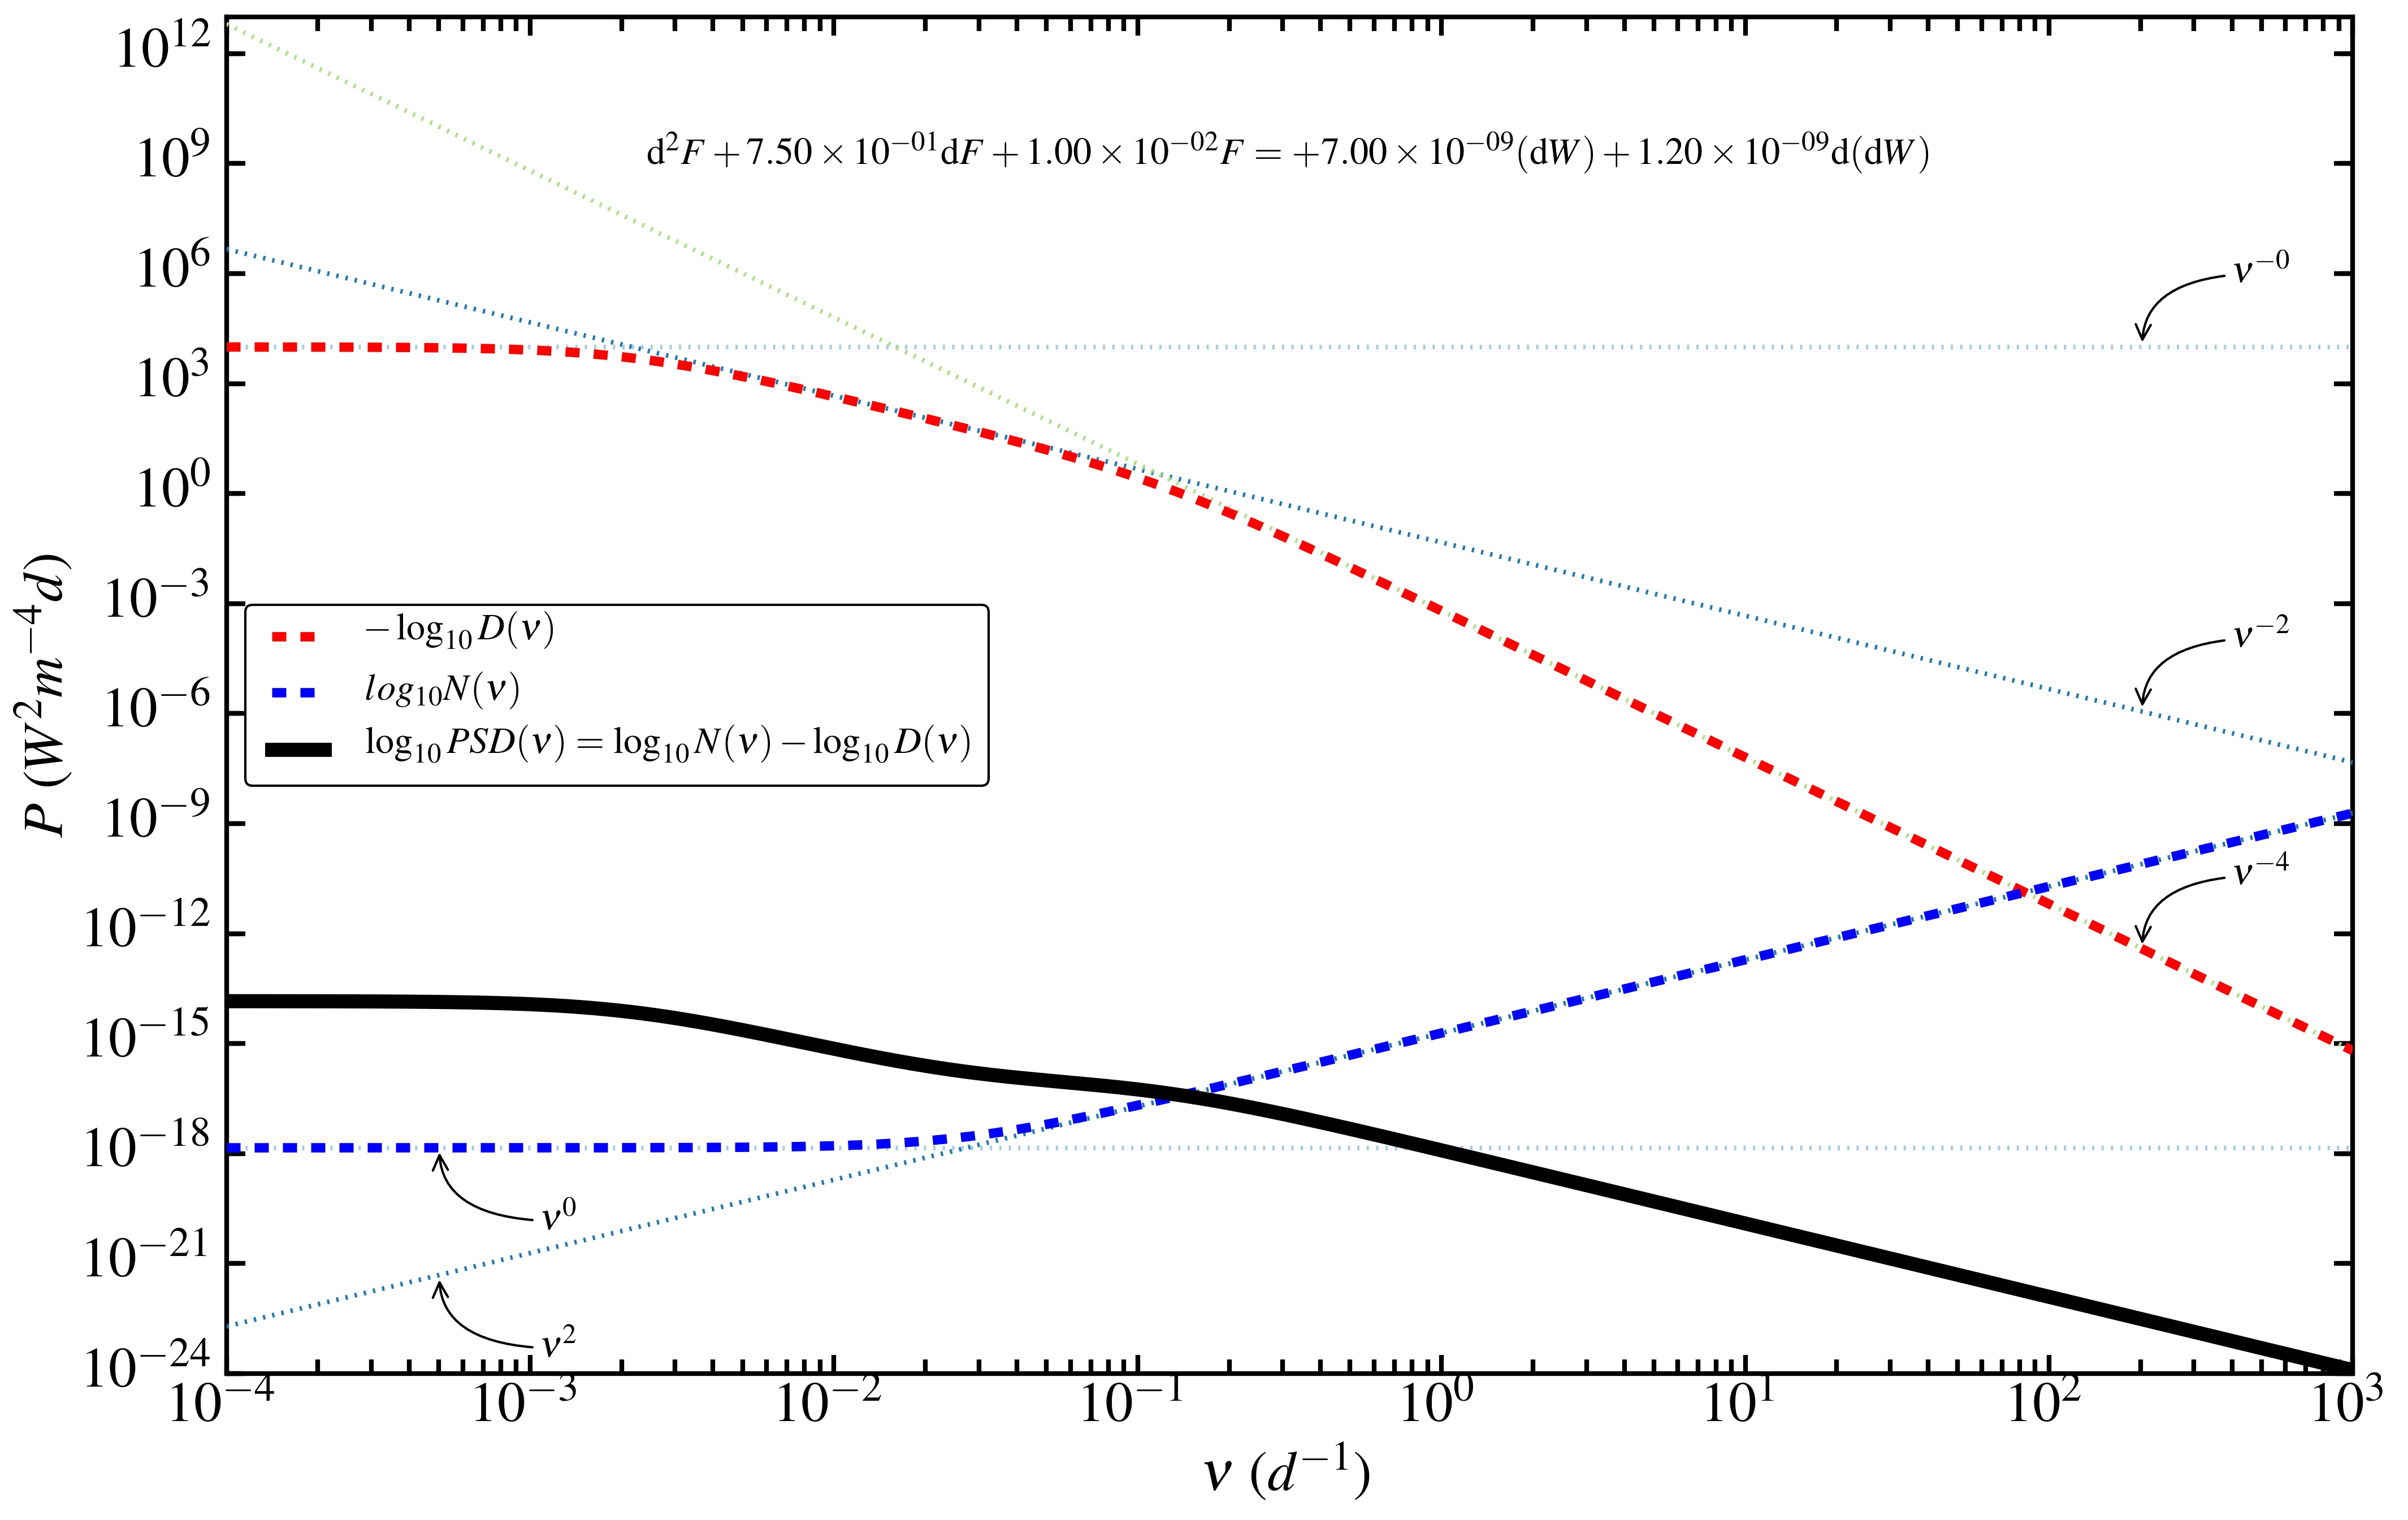
\includegraphics[scale=0.04]{images/CARMA(2,1)_PSD.jpg}
      \end{figure}
    \end{column}
    \begin{column}{0.5\textwidth}
      \begin{figure}
        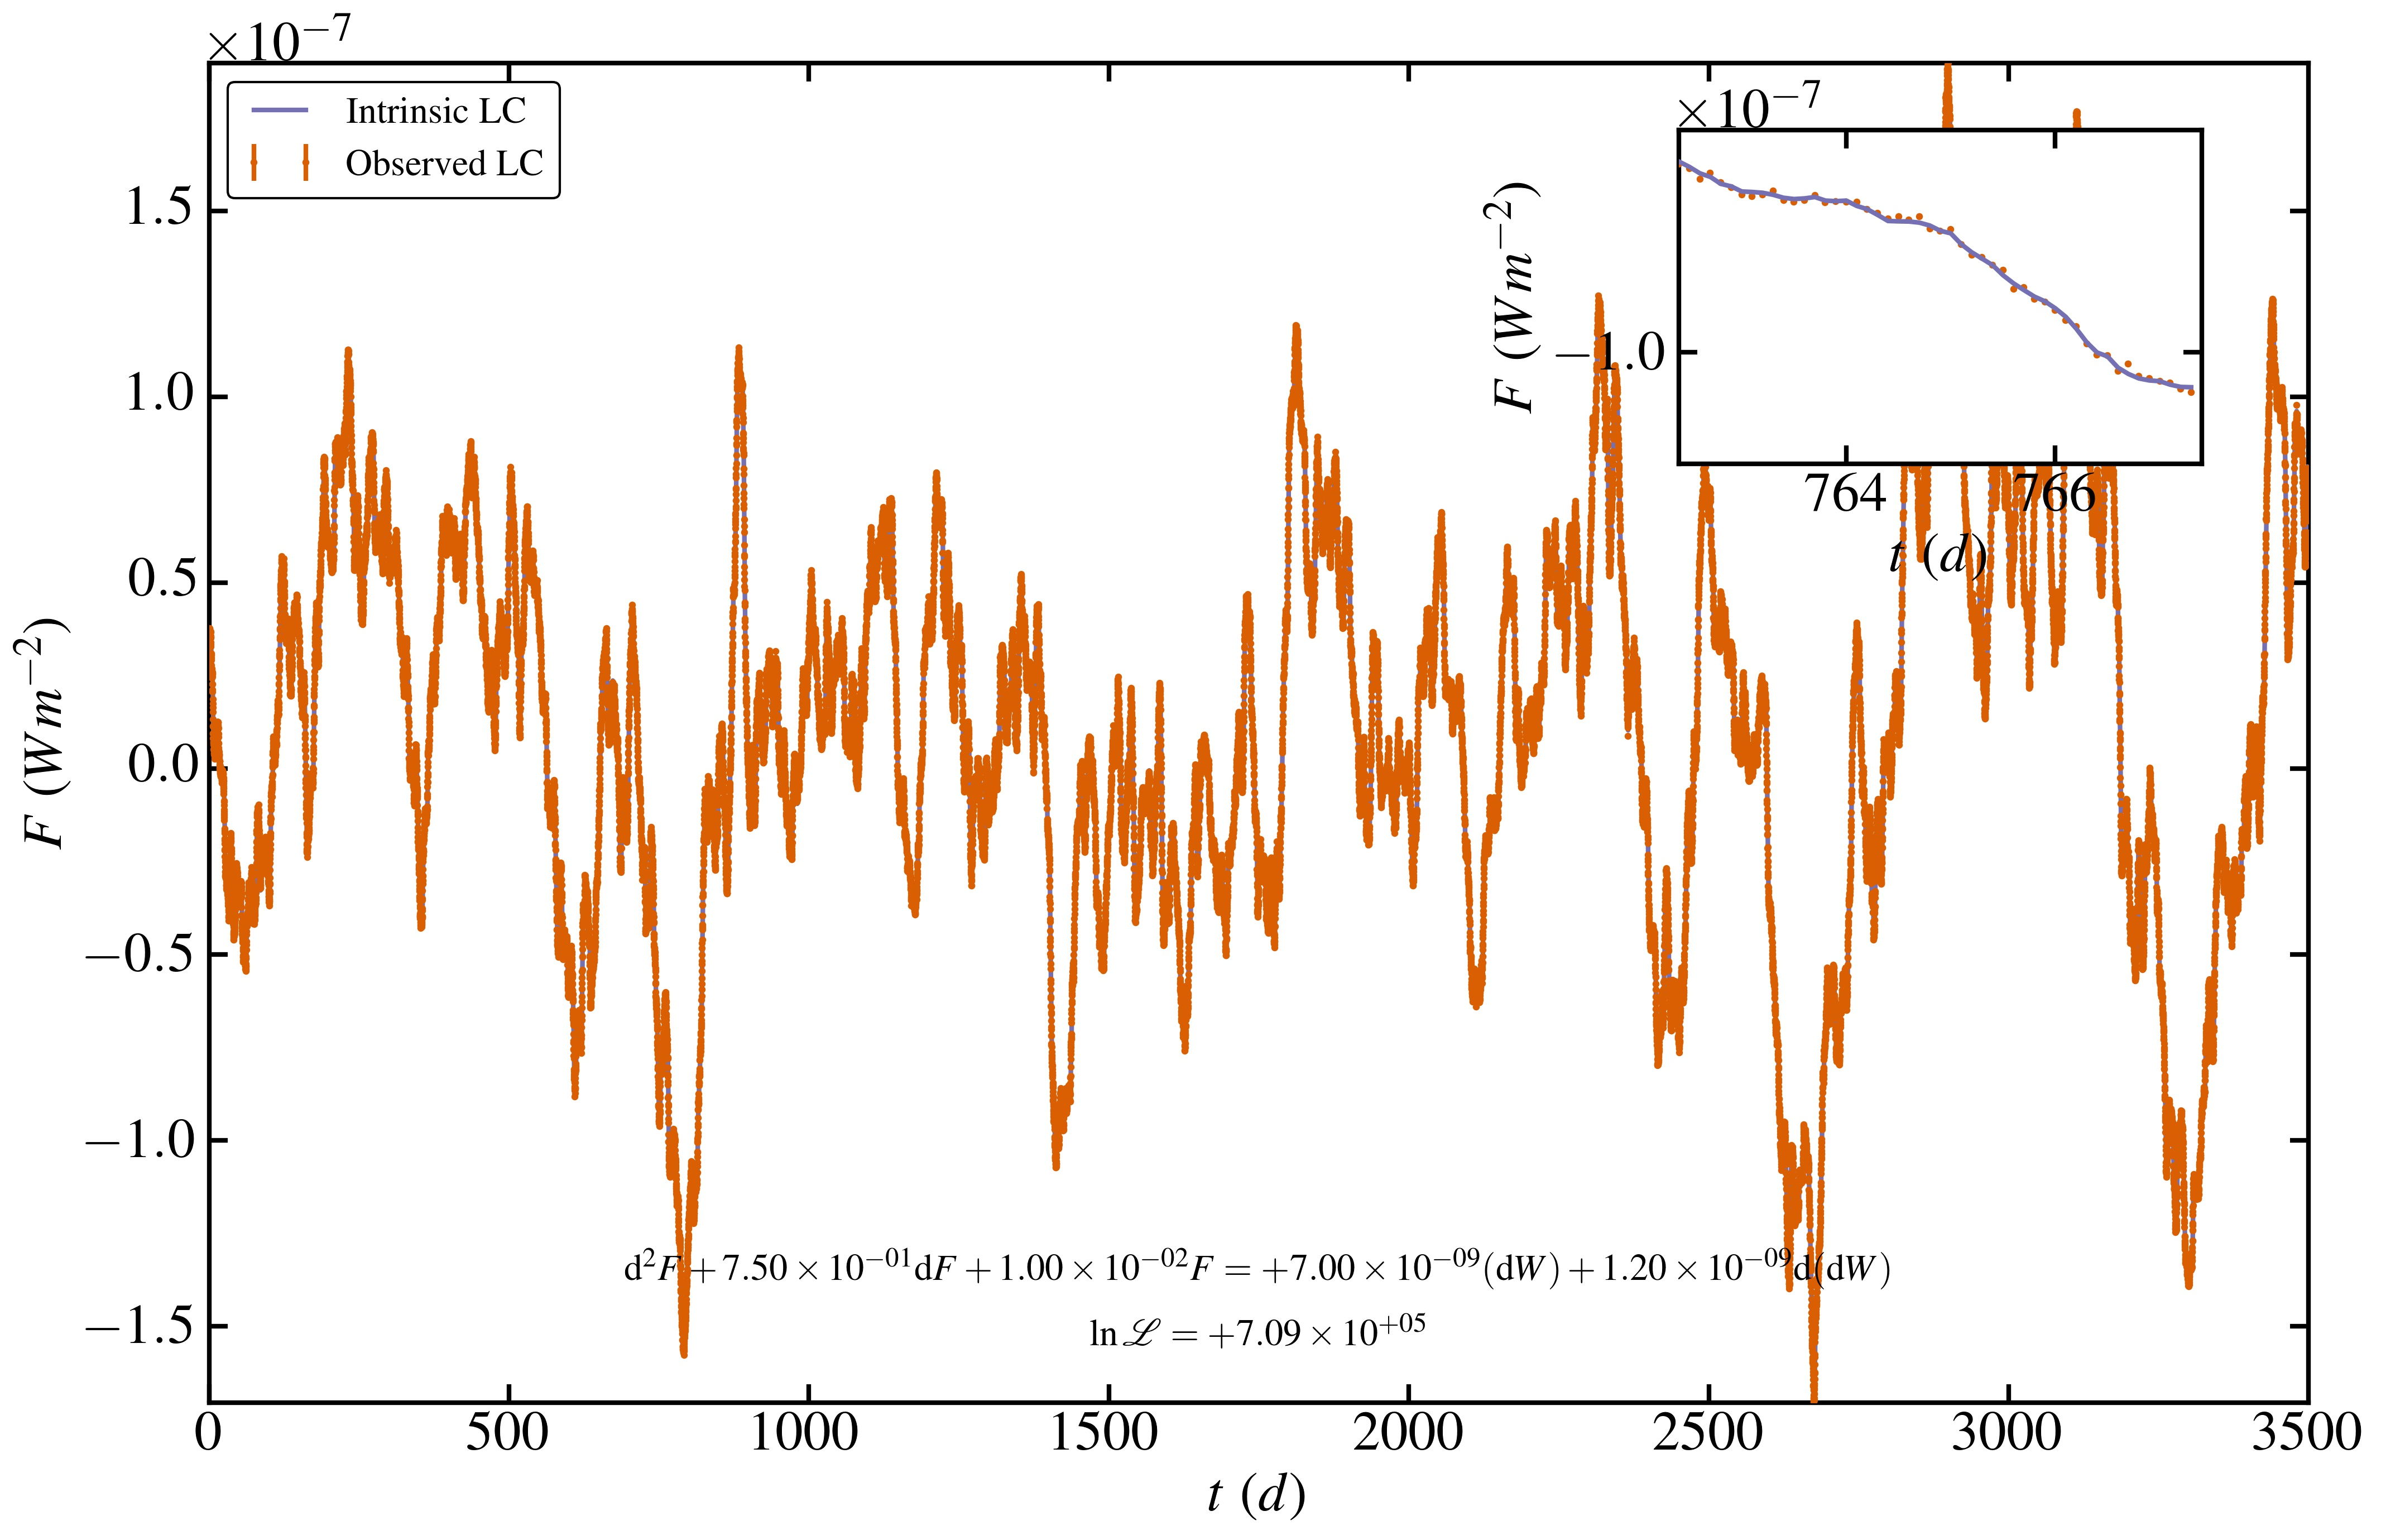
\includegraphics[scale=0.04]{images/CARMA(2,1)_LC.jpg}
      \end{figure}
    \end{column}
  \end{columns}
  %\begin{center}
  %{\tiny \citet*{Kasliwal15b}}
  %\end{center}
\end{frame}


\end{comment}


\begin{frame}
\frametitle{Power Spectral Density\\Eg. C-ARMA($5$,$1$)}
  %\begin{equation*}\label{eq:CARMA21PSD} \mathrm{d}^{2}F + 2\omega\zeta \mathrm{d}F + \omega^{2}F = \beta_{1} \mathrm{d}(\mathrm{d}W) + \beta_{2} (\mathrm{d}W) \end{equation*}
  \begin{columns}
    \begin{column}{0.5\textwidth}
      \begin{figure}
        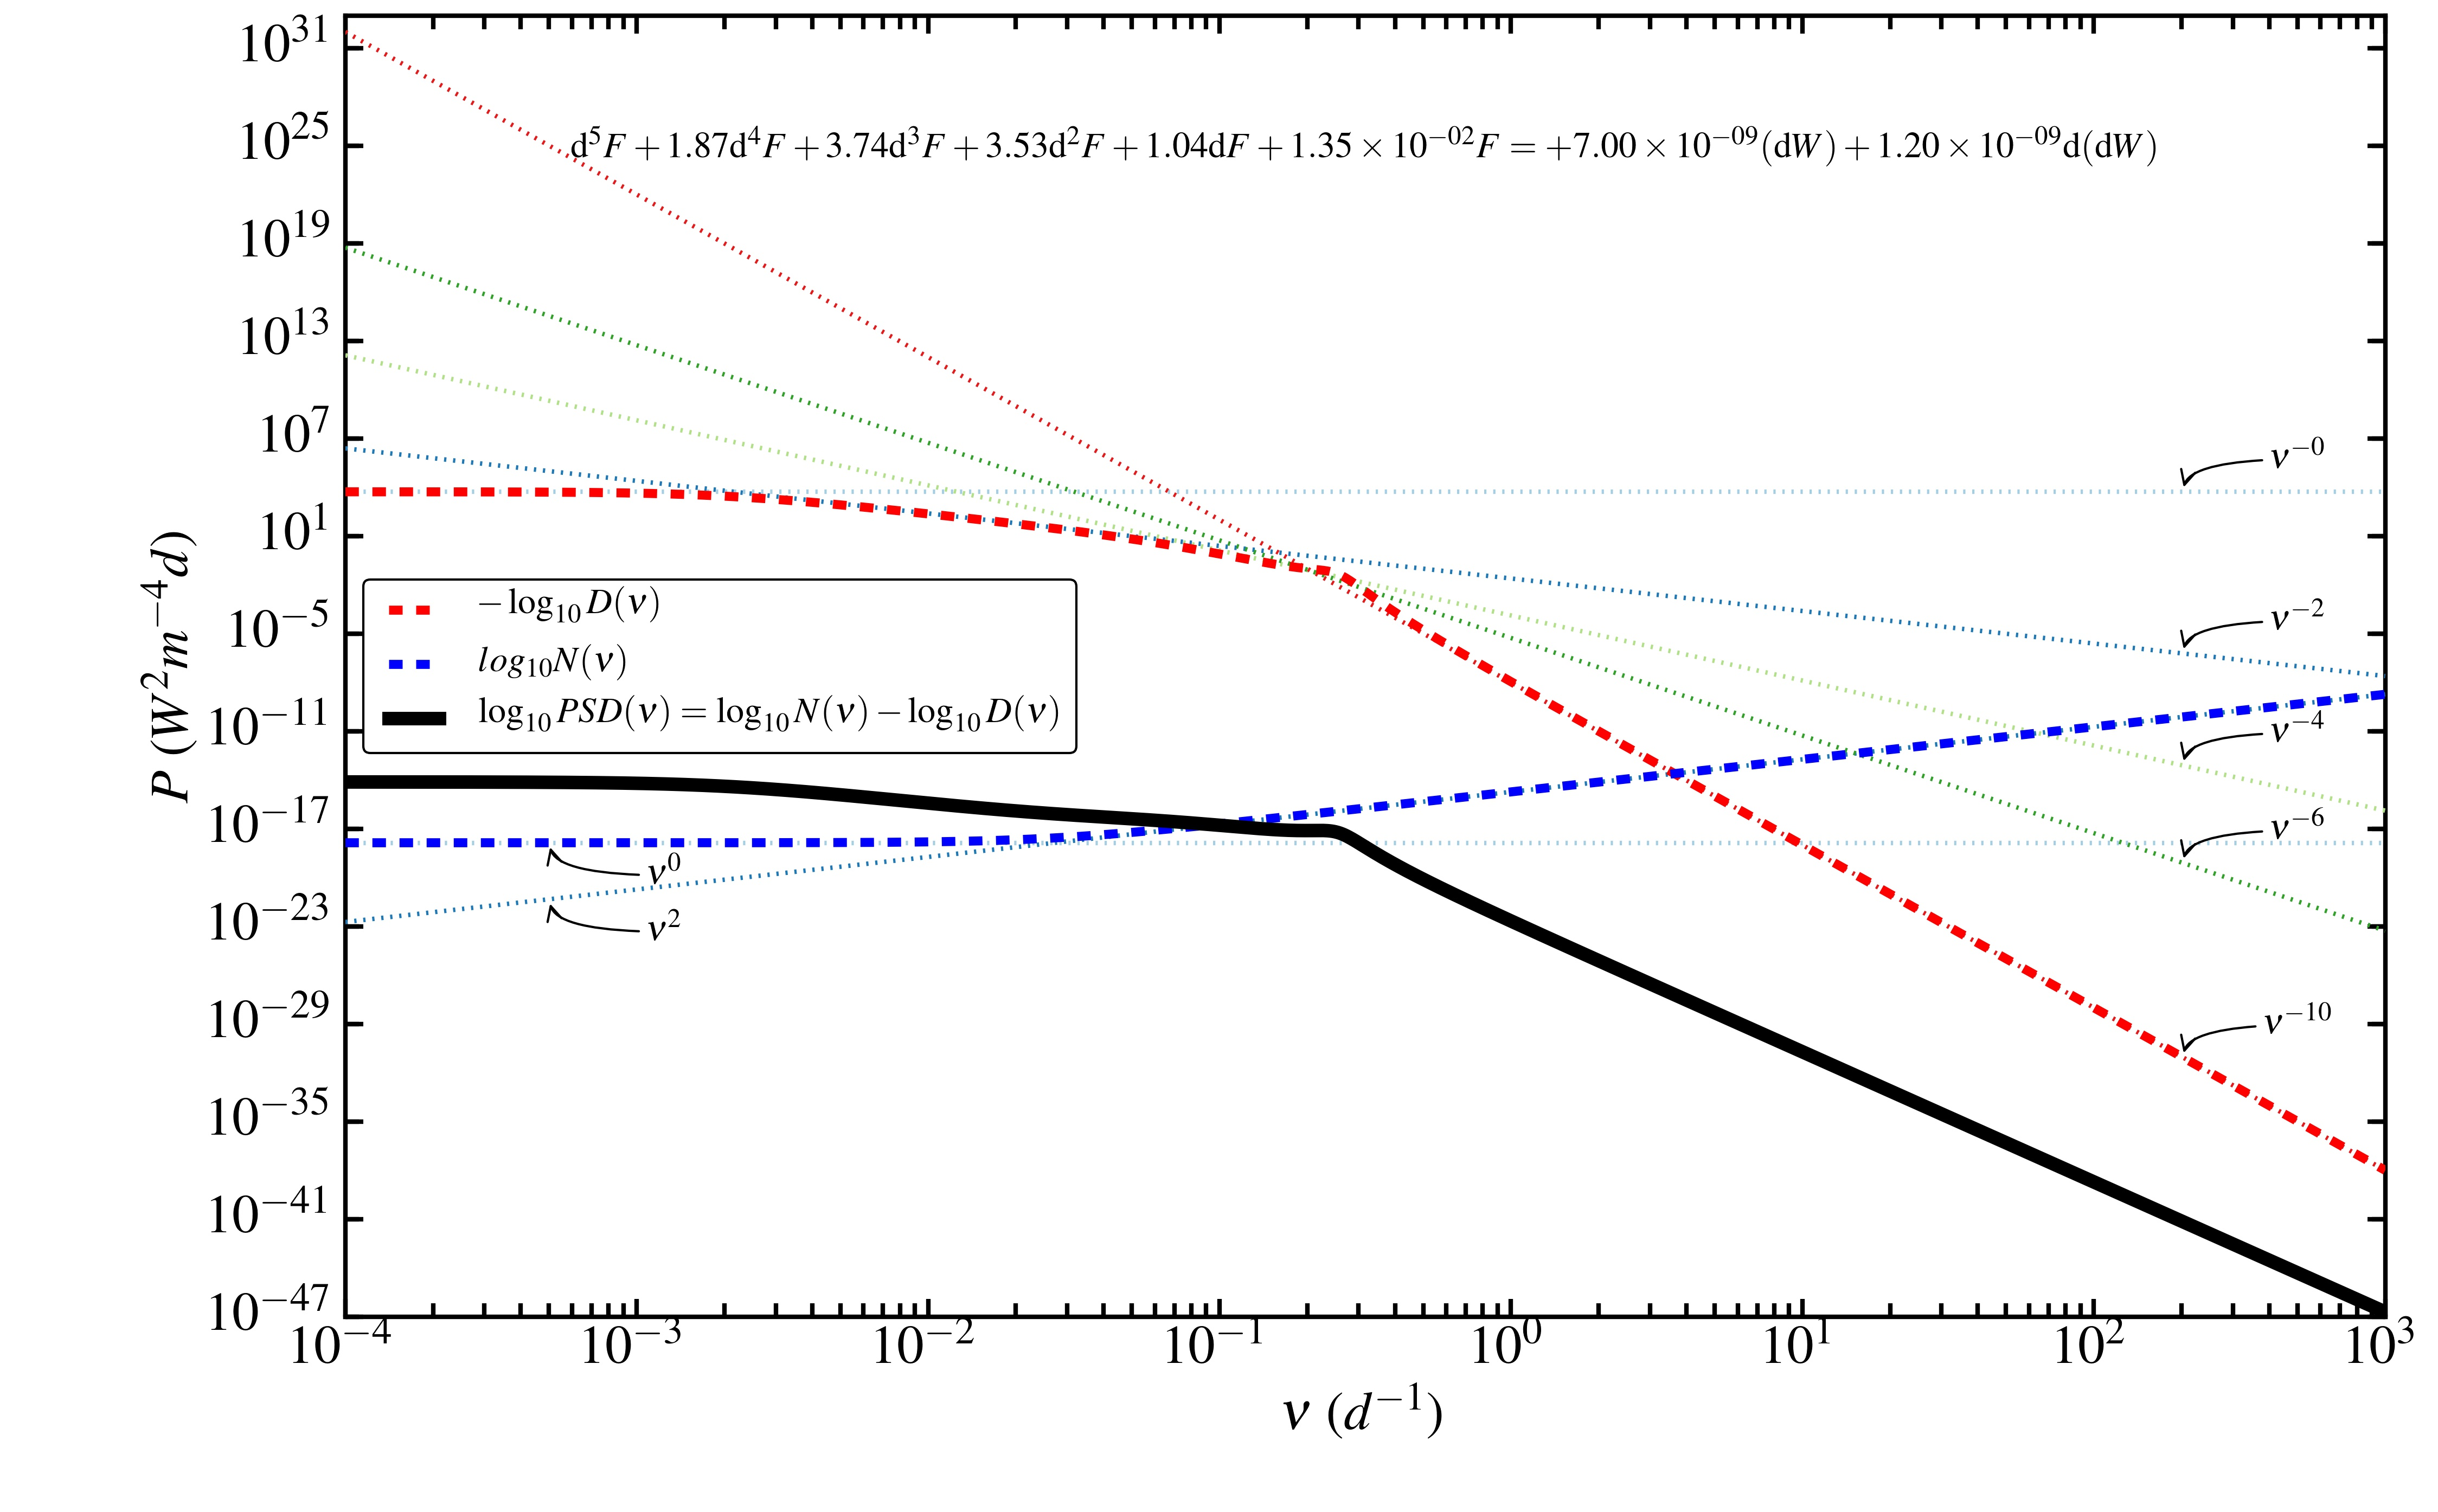
\includegraphics[scale=0.04]{images/CARMA(5,1)_PSD.jpg}
      \end{figure}
    \end{column}
    \begin{column}{0.5\textwidth}
      \begin{figure}
        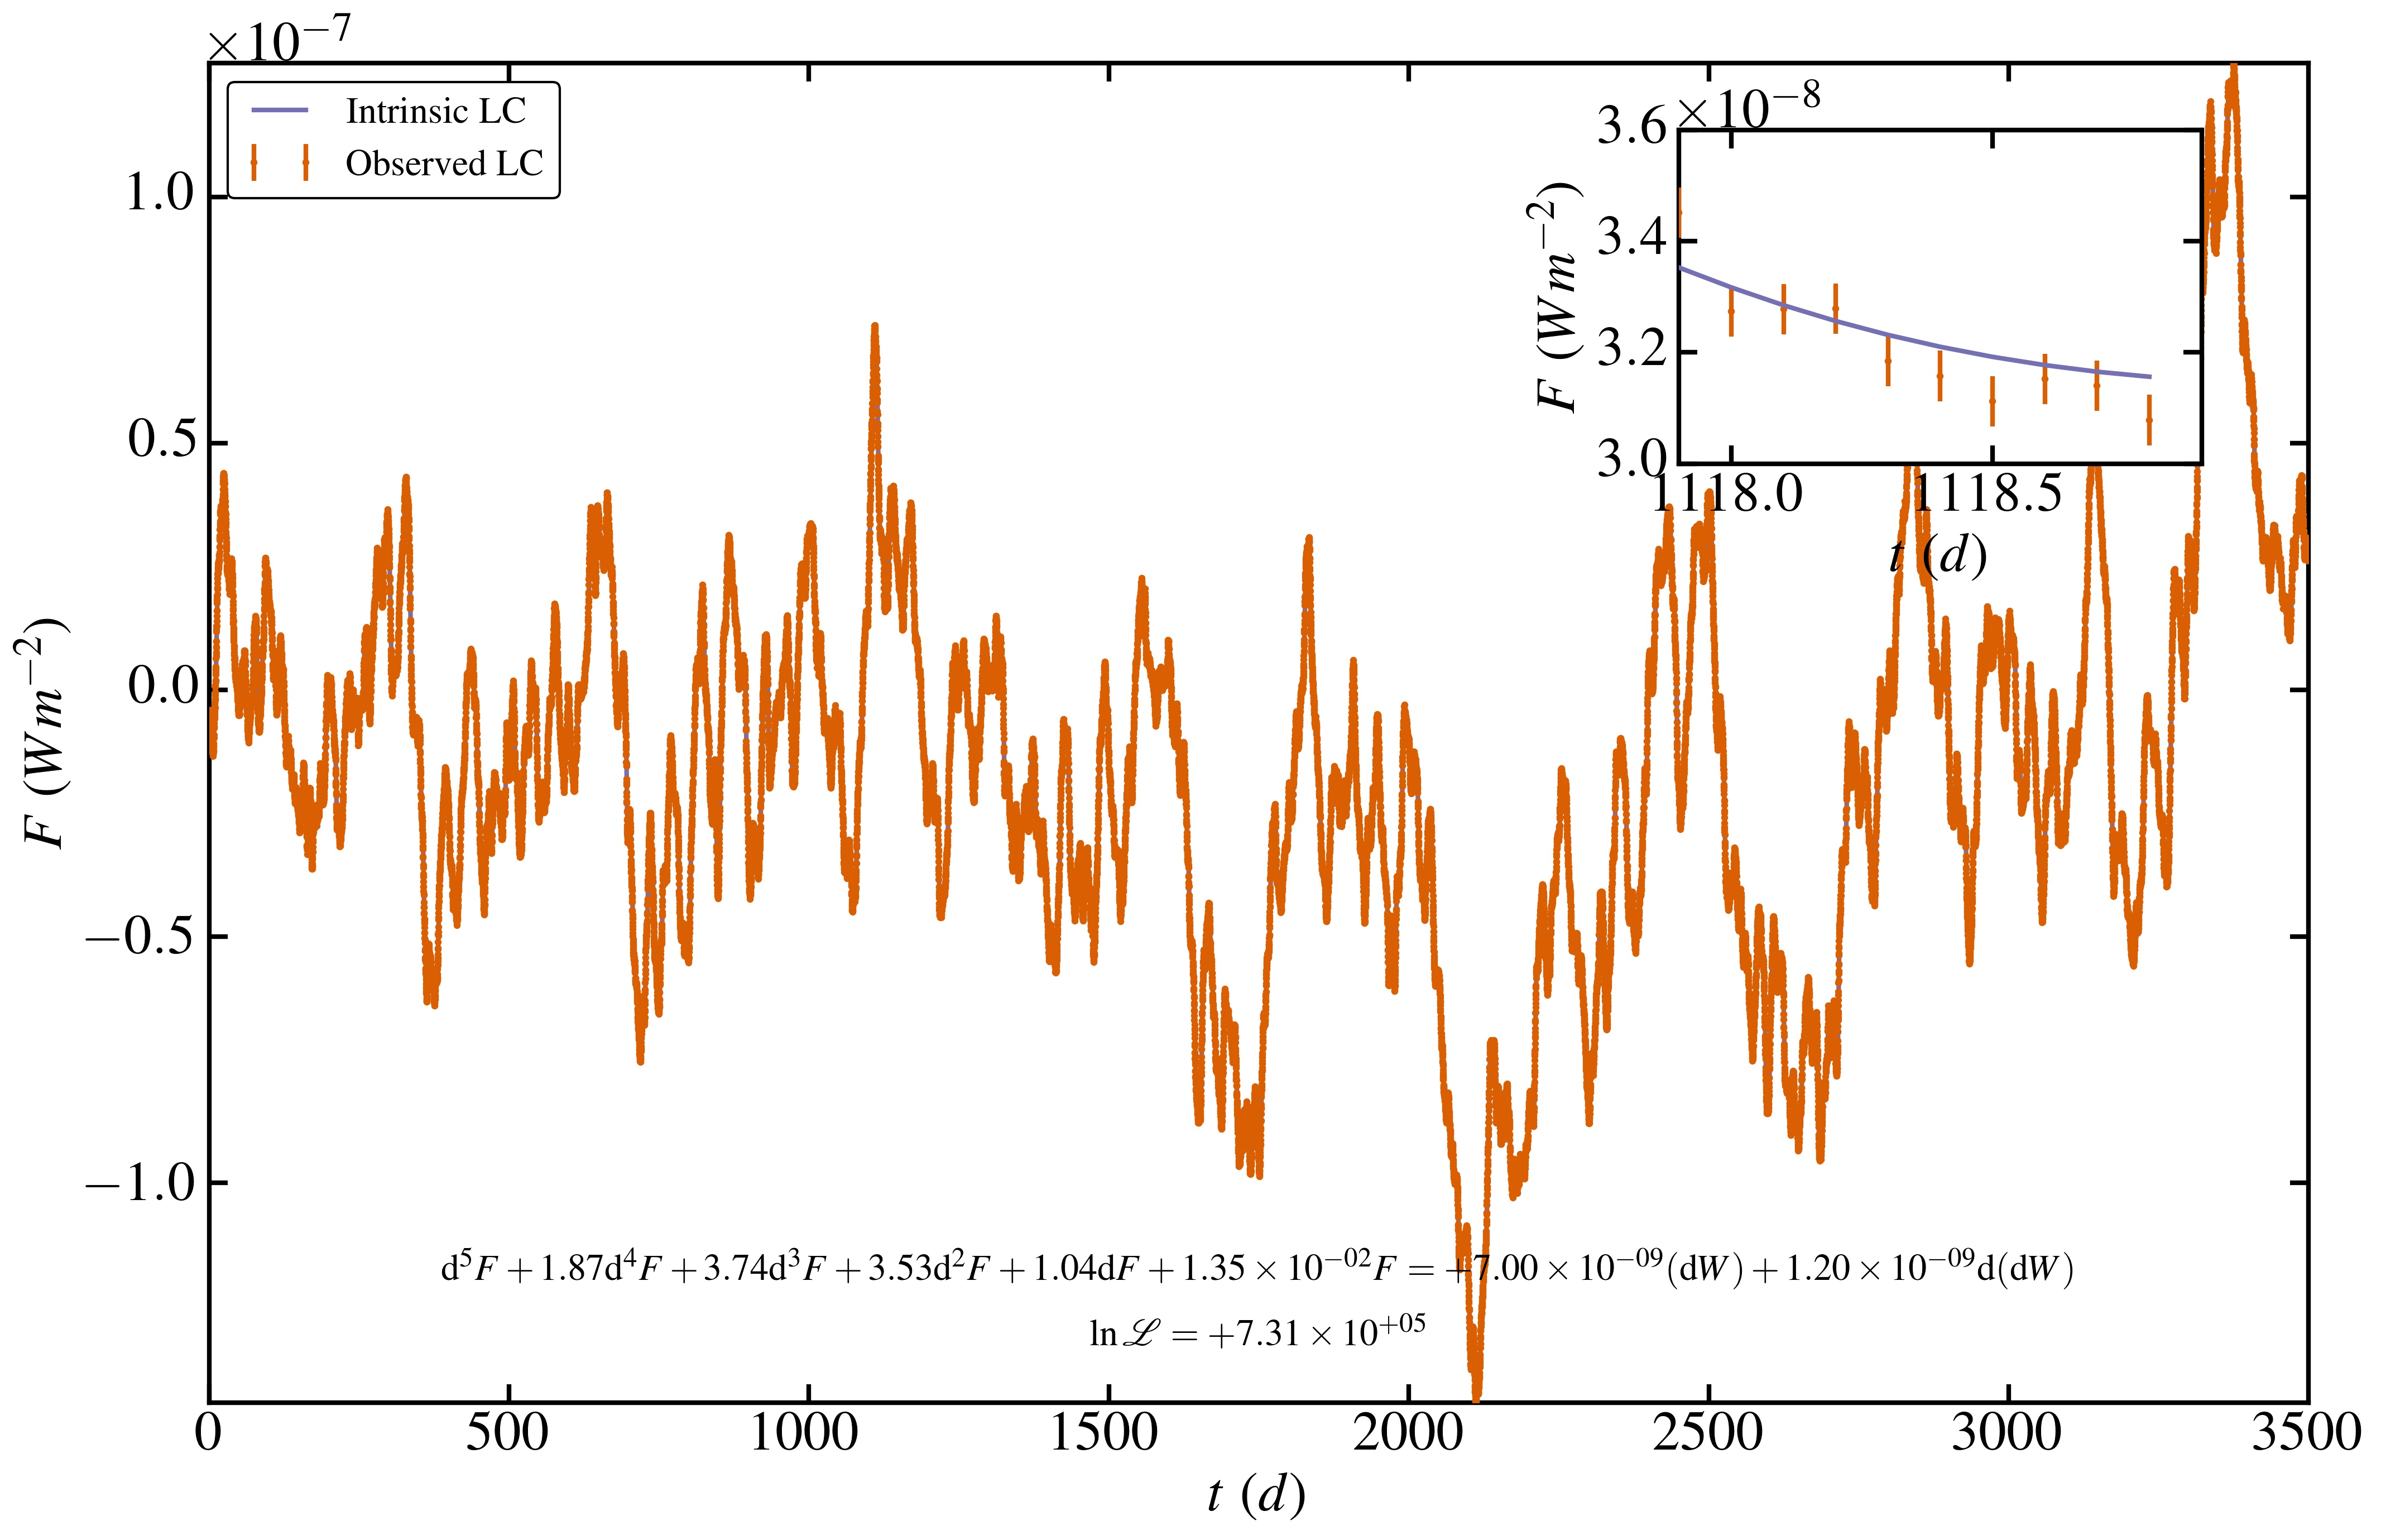
\includegraphics[scale=0.04]{images/CARMA(5,1)_LC.jpg}
      \end{figure}
    \end{column}
  \end{columns}
  %\begin{center}
  %{\tiny \citet*{Kasliwal15b}}
  %\end{center}
\end{frame}

\subsection{Inferencing C-ARMA}


\begin{comment}


\begin{frame}
\frametitle{State Space Representation}
%\begin{equation*}\label{eq:1stCanForm}
%\mathbfss{A} = \left( \begin{array}{ccccc}
%-\alpha_{1} & 1 & \hdots & 0 & 0 \\
%-\alpha_{2} & 0 & \hdots & 0 & 0 \\
%\vdots & \vdots & \ddots & \vdots & \vdots \\
%-\alpha_{p-1} & 0 & \hdots & 0 & 1 \\
%-\alpha_{p} & 0 & \hdots & 0 & 0 \\
%\end{array}\right); \mathbfit{B} = \left( \begin{array}{c} \beta_{1} \\ \beta_{2} \\ \vdots \\ \beta_{p-1} \\ \beta_{p} \end{array} \right); \mathbfss{H} = \left( \begin{array}{c} 1 \\ 0 \\ \vdots \\ 0 \\ 0 \end{array} \right)^{\top}.
%\end{equation*}

  %\begin{equation*}\label{eq:StateEqn} \mathrm{d}\mathbfit{x} = \mathbfss{A}\mathbfit{x}\mathrm{d}t + \mathbfit{B}\mathrm{d}w \end{equation*}
  %\begin{equation*}\label{eq:ObsEqn} y = \mathbfss{H}\mathbfit{x} \end{equation*}

  %\begin{equation*}\label{eq:TransMat} \mathbfss{F} = \mathrm{e}^{\mathbfss{A}\delta t} \end{equation*}
  %\begin{equation*}\label{eq:DistMat} \mathbfss{Q} = \int_{0}^{\delta t} \mathrm{e}^{\mathbfss{A}\xi}\mathbfit{B}\mathbfit{B}^{\top}\mathrm{e}^{\mathbfss{A}^{\top}\xi} d\xi \end{equation*}

  State equation: \begin{equation*}\label{eq:ARMAStateEq}
  \mathrm{d}\mathbfit{x}(t) = \mathbfss{A}\mathbfit{x} + \mathbfit{B}\mathrm{d}W \xrightarrow{\mathrm{integrate \ \& \ sample}} \mathbfit{x}_{k+1} = \mathbfss{F}\mathbfit{x}_{k} + \mathbfit{w}_{k} \end{equation*}
    with
  \begin{equation*}\label{eq:ARMADisturbance} \mathbfss{F} = \mathrm{e}^{\mathbfss{A}\delta t}; \mathbfit{w}_{k} \sim \mathcal{N}(\mathbfit{0},\mathbfss{Q}); \mathbfss{Q} = \int_{0}^{\delta t} \mathrm{e}^{\mathbfss{A}\xi} \mathbfit{B} \mathbfit{B}^{\top} \mathrm{e}^{\mathbfss{A}^{\top}\xi} \mathrm{d} \xi
  \end{equation*}
  %\begin{equation*}\label{eq:QInt} \mathbfss{Q} = \int_{0}^{\delta t} \mathrm{e}^{\mathbfss{A}\xi} \mathbfit{B} \mathbfit{B}^{\top} \mathrm{e}^{\mathbfss{A}^{\top}\xi} \mathrm{d} \xi
  %\end{equation*}

  Observation equation: \begin{equation*}\label{eq:ARMAObsEqn} x_{k, \mathrm{obs}} = \mathbfss{H}_{k}\mathbfit{x}_{k} + v_{k} \end{equation*}
  \begin{equation*}\label{eq:ARMANoise} v_{k} \sim \mathcal{N}(0,\sigma^{2}_{N,k}) \end{equation*}

  \begin{itemize}
    \item $\mathbfss{F}$: Transition matrix \& $\mathbfss{Q}$: Disturbance matrix
    \item $\mathbfss{H}$: Observation matrix
    \item Observation noise in-built via $v_{k}$!
    \item Well studied by engineers (Control systems) and economists
  \end{itemize}
\end{frame}

\begin{frame}
\frametitle{Evolution \& observation of light curve state}
  \begin{center}
    \centering
    \movie[externalviewer]{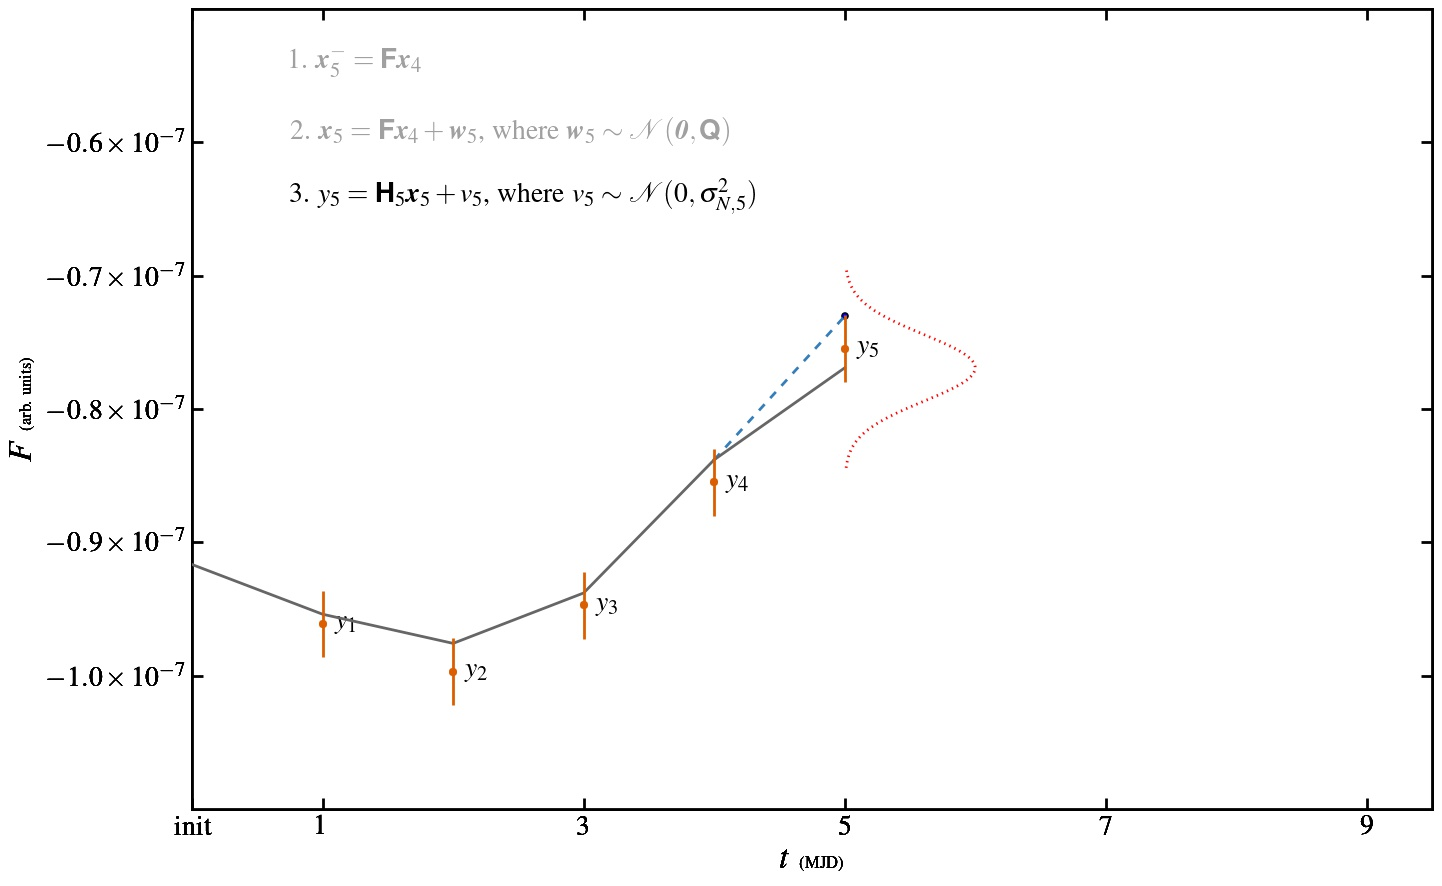
\includegraphics[scale=0.2]{images/Fig0_Pt5_Step4.jpg}}{LC2.mp4}
        %\href{http://168.176.8.14/sagan/TipoAGN.html}{{\tiny Columbian National University: Bogota}}
  \end{center}
  %\begin{center}
    %\centering
    %{\tiny \citet{ArmitageReynolds03}}
  %\end{center}
\end{frame}

\subsection{Model Inferencing}

\begin{frame}
\frametitle{The Kalman Filter}
  \begin{itemize}
    \item Linear quadratic estimator of $\mathbfit{x}$.
    \item Kalman filter + Linear-quadratic regulator (LQR) = Linear-quadratic Gaussian control: First used to guide Apollo.
    \item Predictor-Corrector algorithm.
    \item \textbf{Predict}: Where should the system go?
    \item \textbf{Compute}: Compute the log-likelihood of the data given the prediction.
    \item \textbf{Correct}: Update the system based on the prediction \& observation.
  \end{itemize}
\end{frame}

\begin{frame}
\frametitle{$\ln \mathcal{L}$ via Kalman filter}
  \begin{center}
    \centering
    \movie[externalviewer]{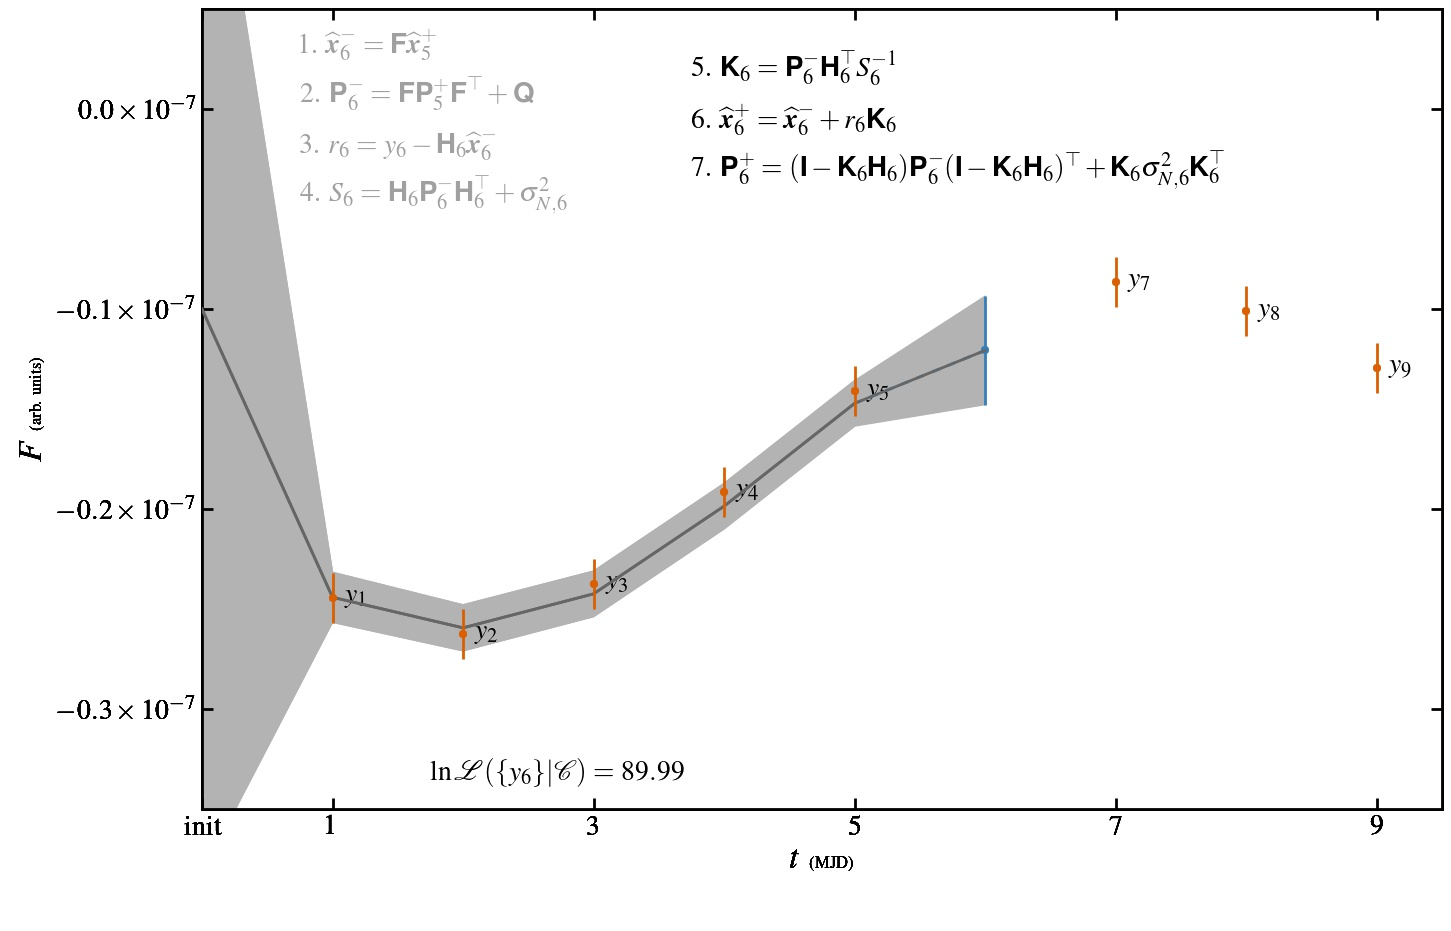
\includegraphics[scale=0.2]{images/Fig1_Pt5_Step5.jpg}}{LnLike2.mp4}
        %\href{http://168.176.8.14/sagan/TipoAGN.html}{{\tiny Columbian National University: Bogota}}
  \end{center}
  %\begin{center}
    %\centering
    %{\tiny \citet{ArmitageReynolds03}}
  %\end{center}
\end{frame}


\end{comment}


\begin{frame}
\frametitle{Confidence Interval Estimates}
  \begin{figure}
    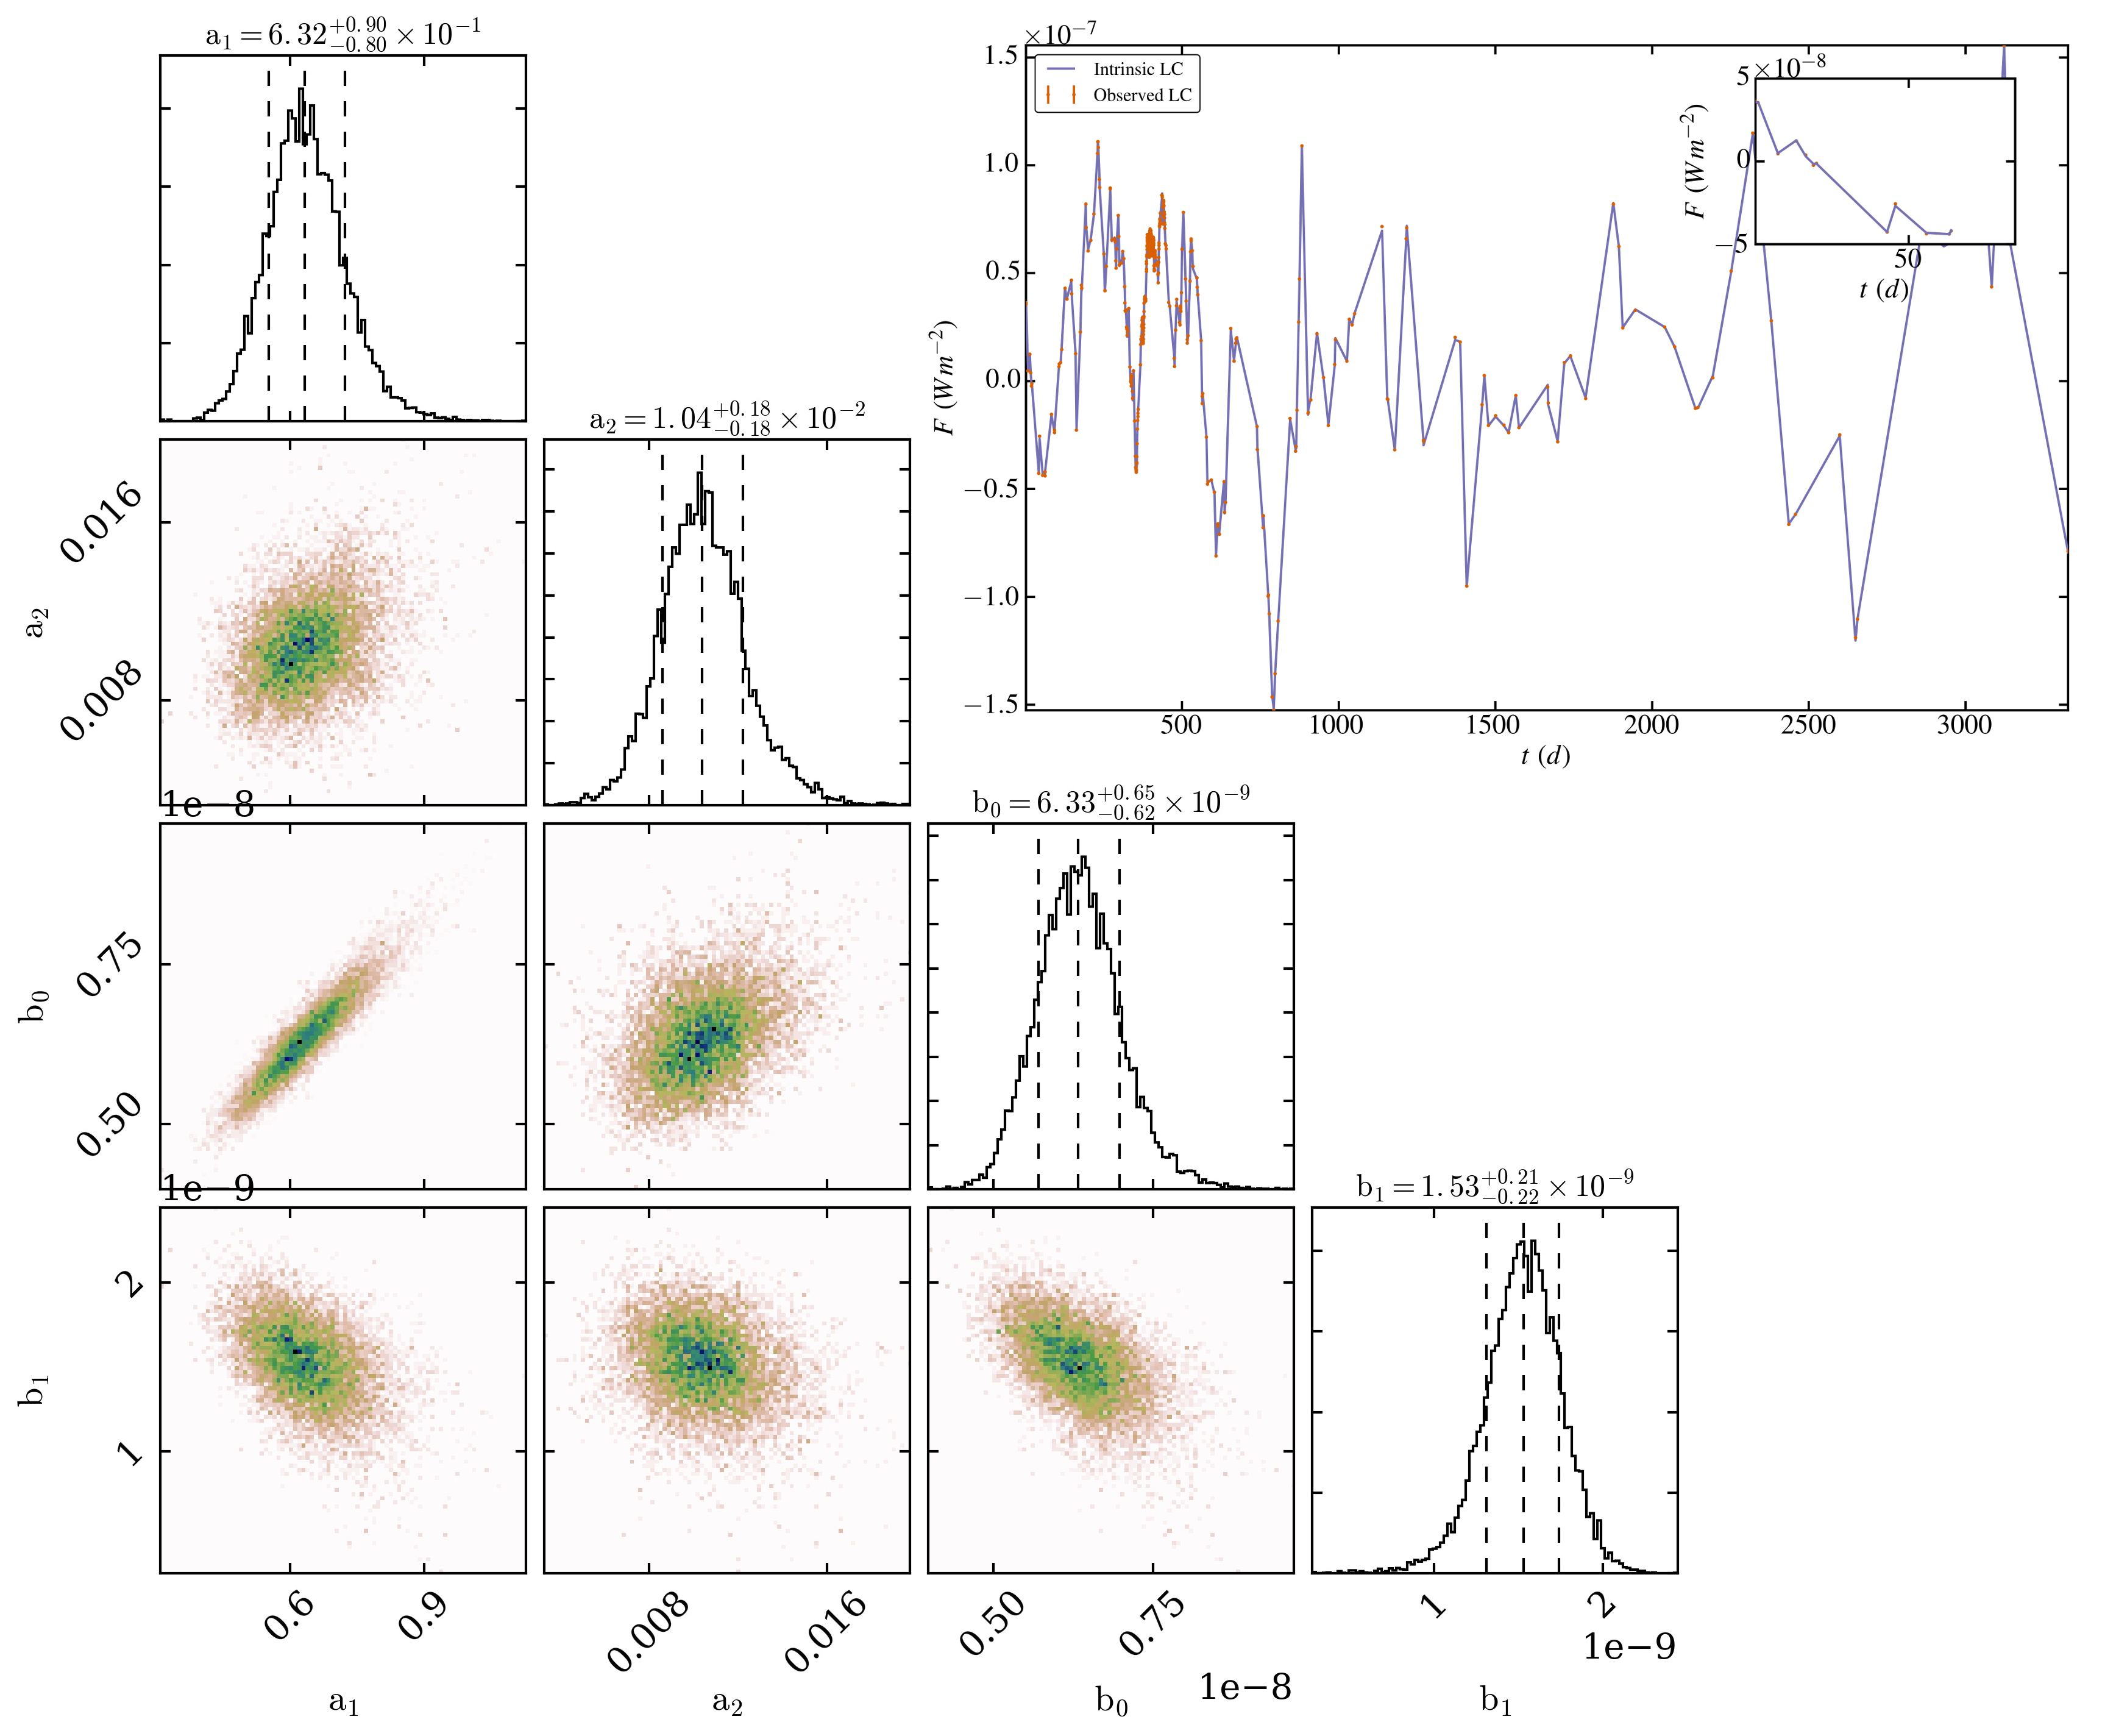
\includegraphics[scale=0.075]{images/CARMA(2,1)_Recovery.jpg}
  \end{figure}
\end{frame}


\begin{comment}


\begin{frame}
\frametitle{Smoothed Light Curve}
  \begin{figure}
    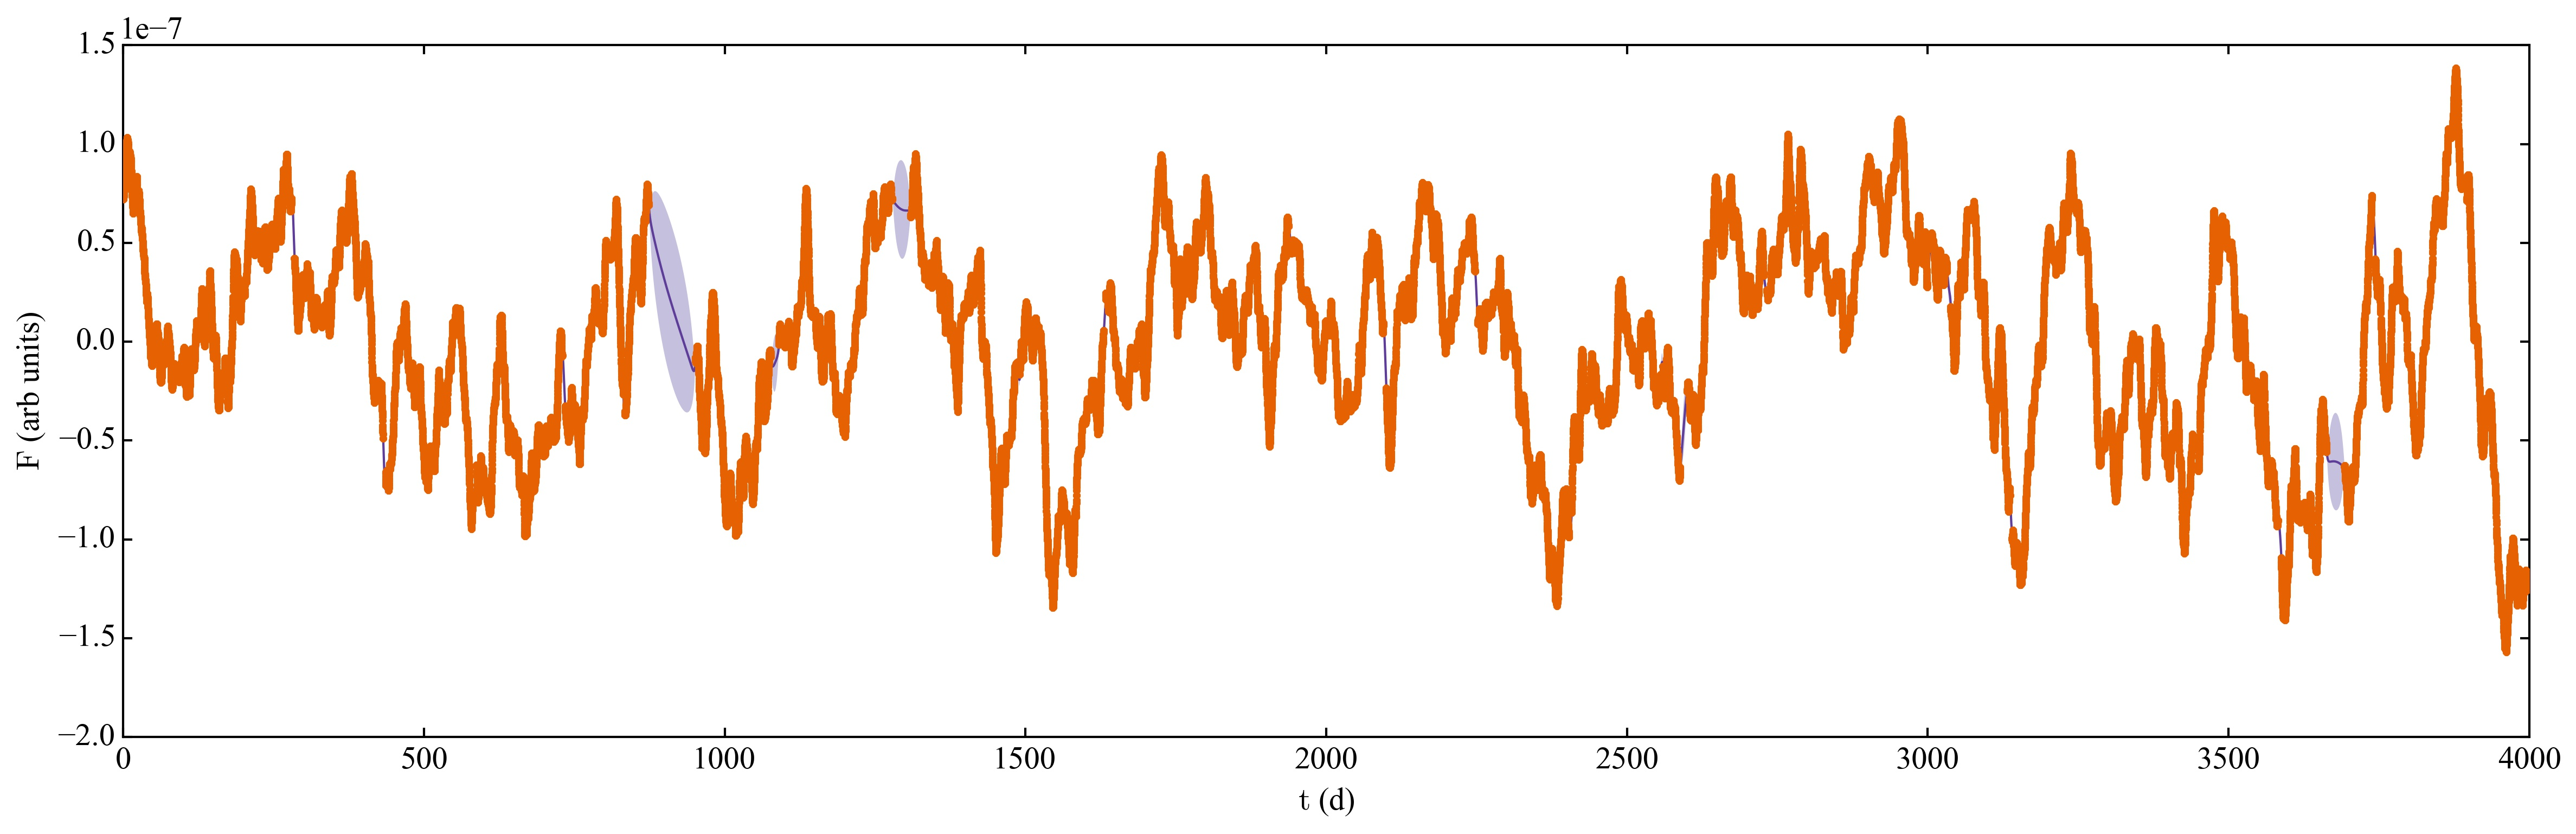
\includegraphics[scale=0.0725]{images/CARMA(2,2)_MCMCFit.jpg}
  \end{figure}
\end{frame}


\end{comment}


\subsection{Interpreting C-ARMA}

\begin{frame}
\frametitle{How to Interpret?: Green's Function of LHS\\(eg. C-ARMA($2$,$1$)...)}
  \begin{equation*}\label{eq:CARMAGF} \mathrm{d}^{2}G + 2\omega\zeta \mathrm{d}G + \omega^{2}G = \delta(0) \end{equation*}
  \begin{figure}
    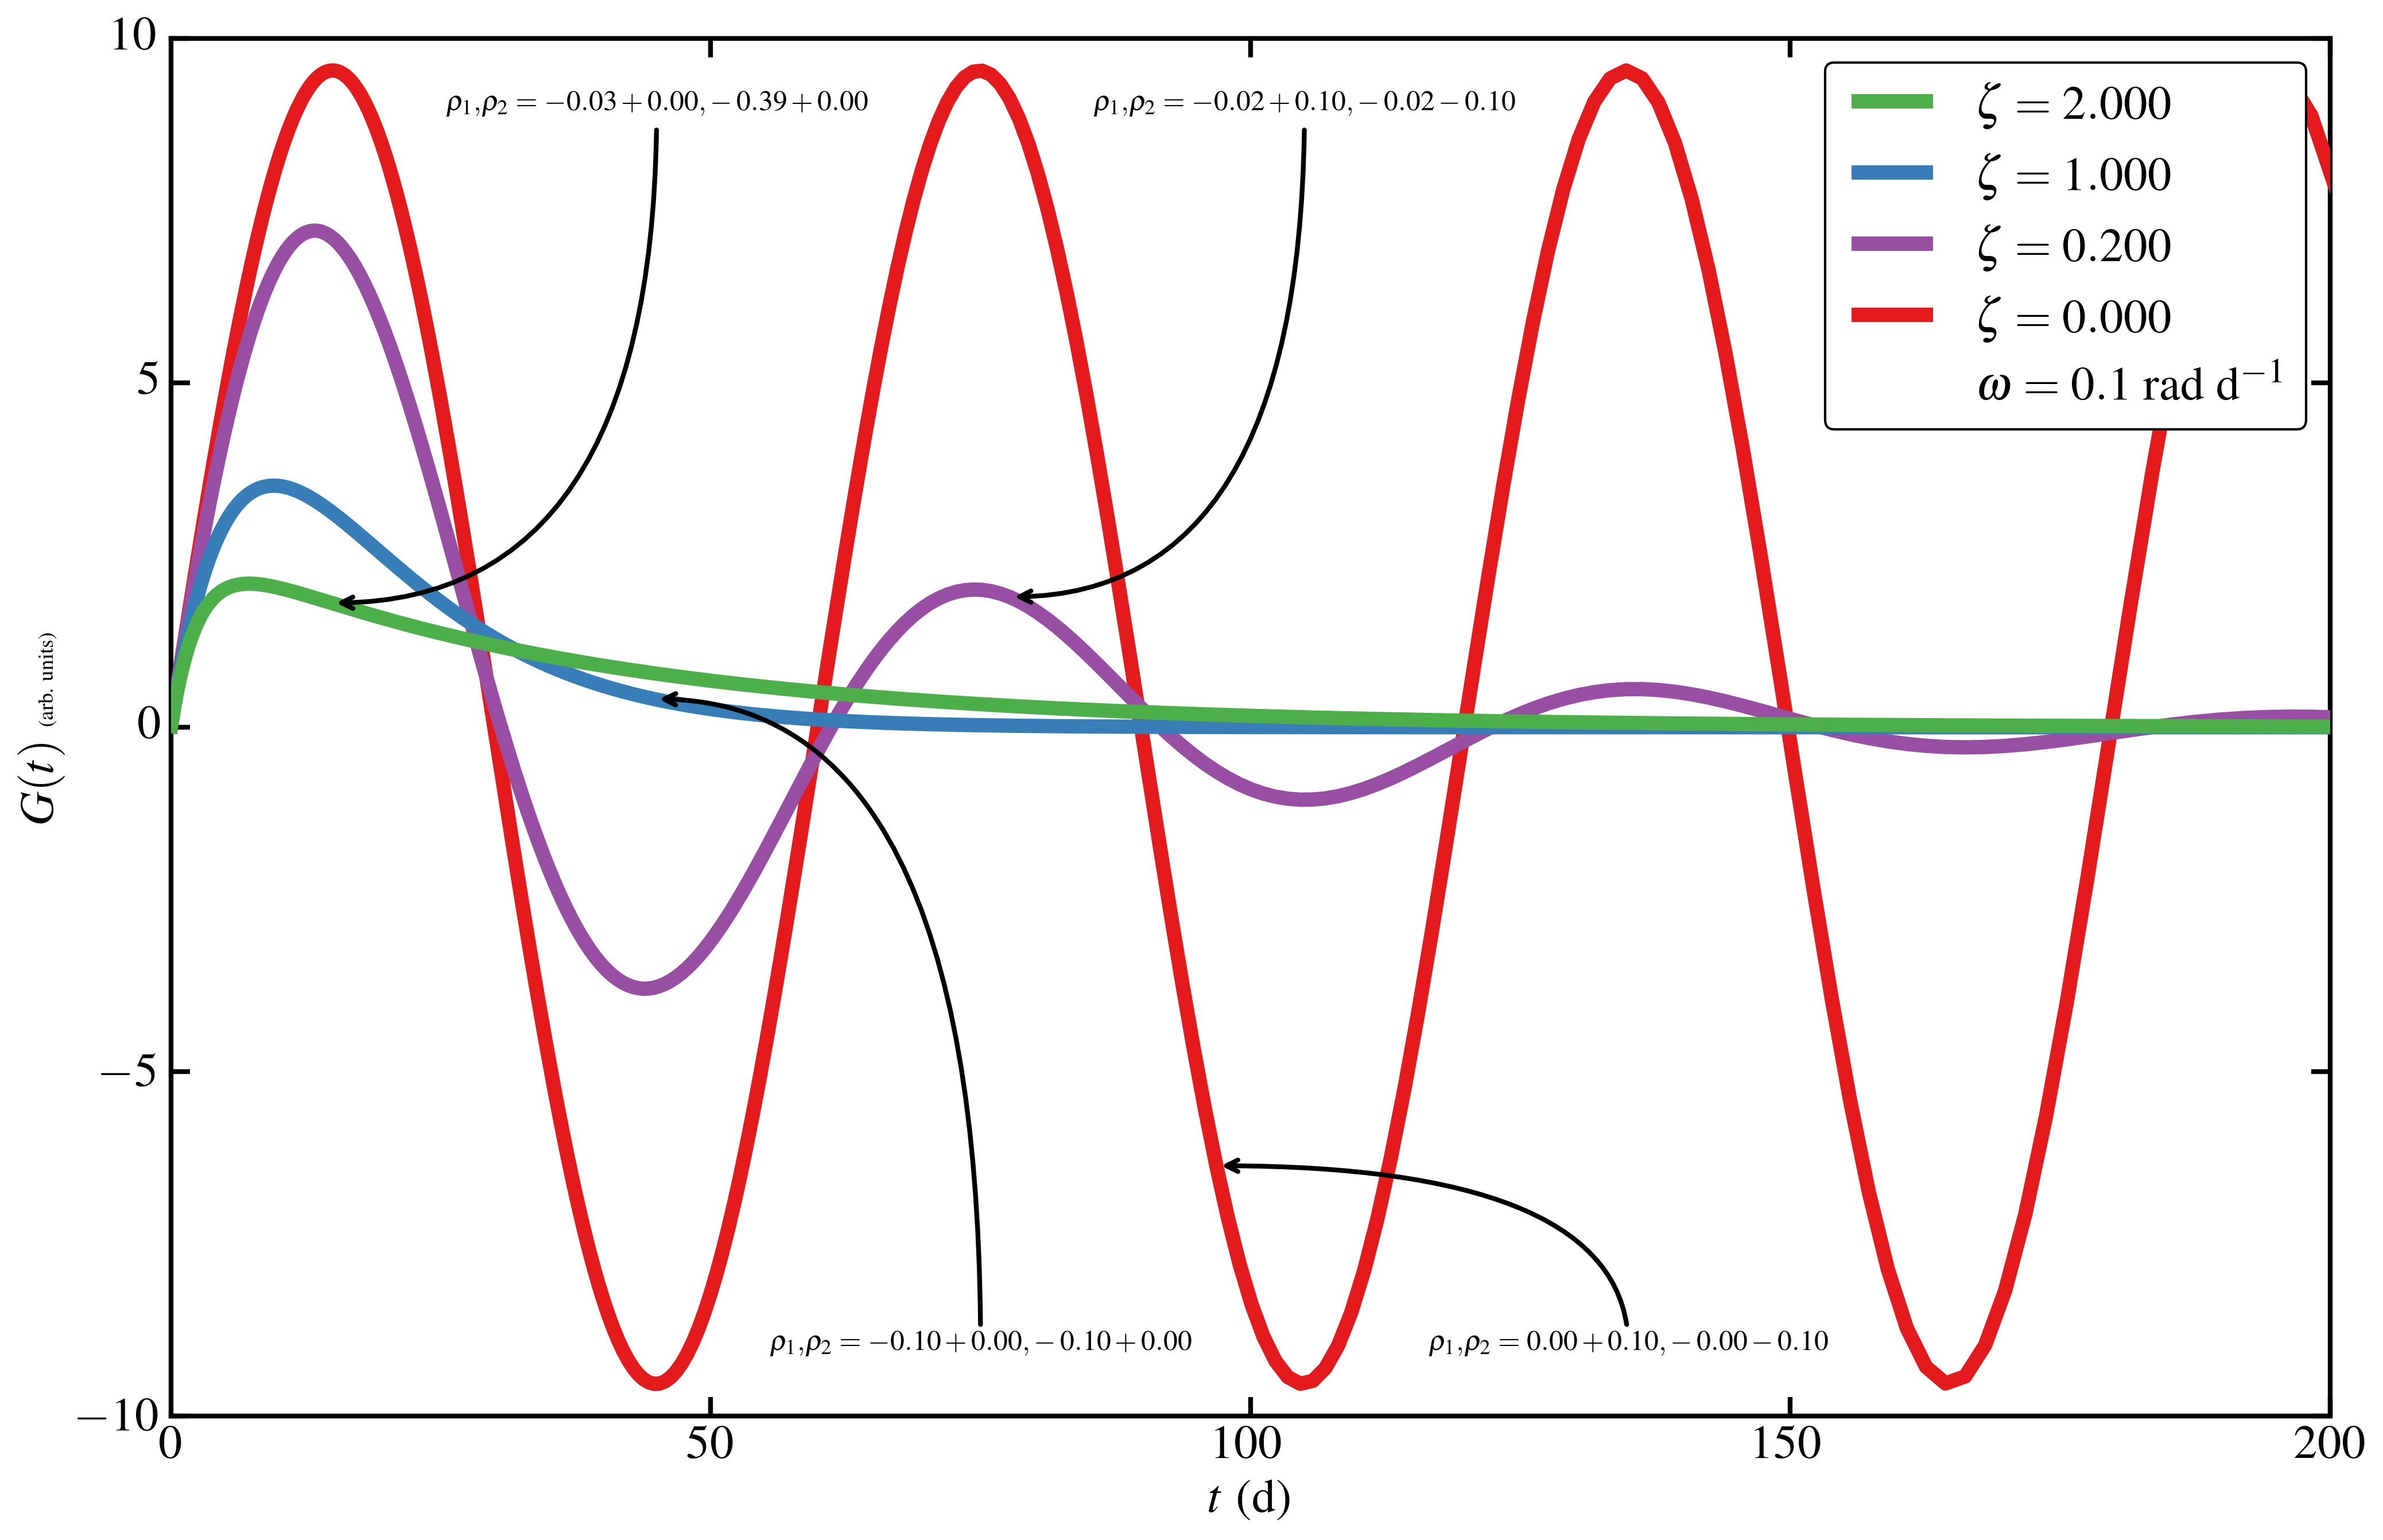
\includegraphics[scale=0.06]{images/CARMA(2,1)_GF.jpg}
  \end{figure}
  %\begin{center}
  %{\tiny \citet*{Kasliwal15b}}
  %\end{center}
\end{frame}

\subsection{C-ARMA Analysis of Zw 229-15}

\begin{frame}
\frametitle{Zw 229-15 (kplr006932990)}
  \begin{figure}
    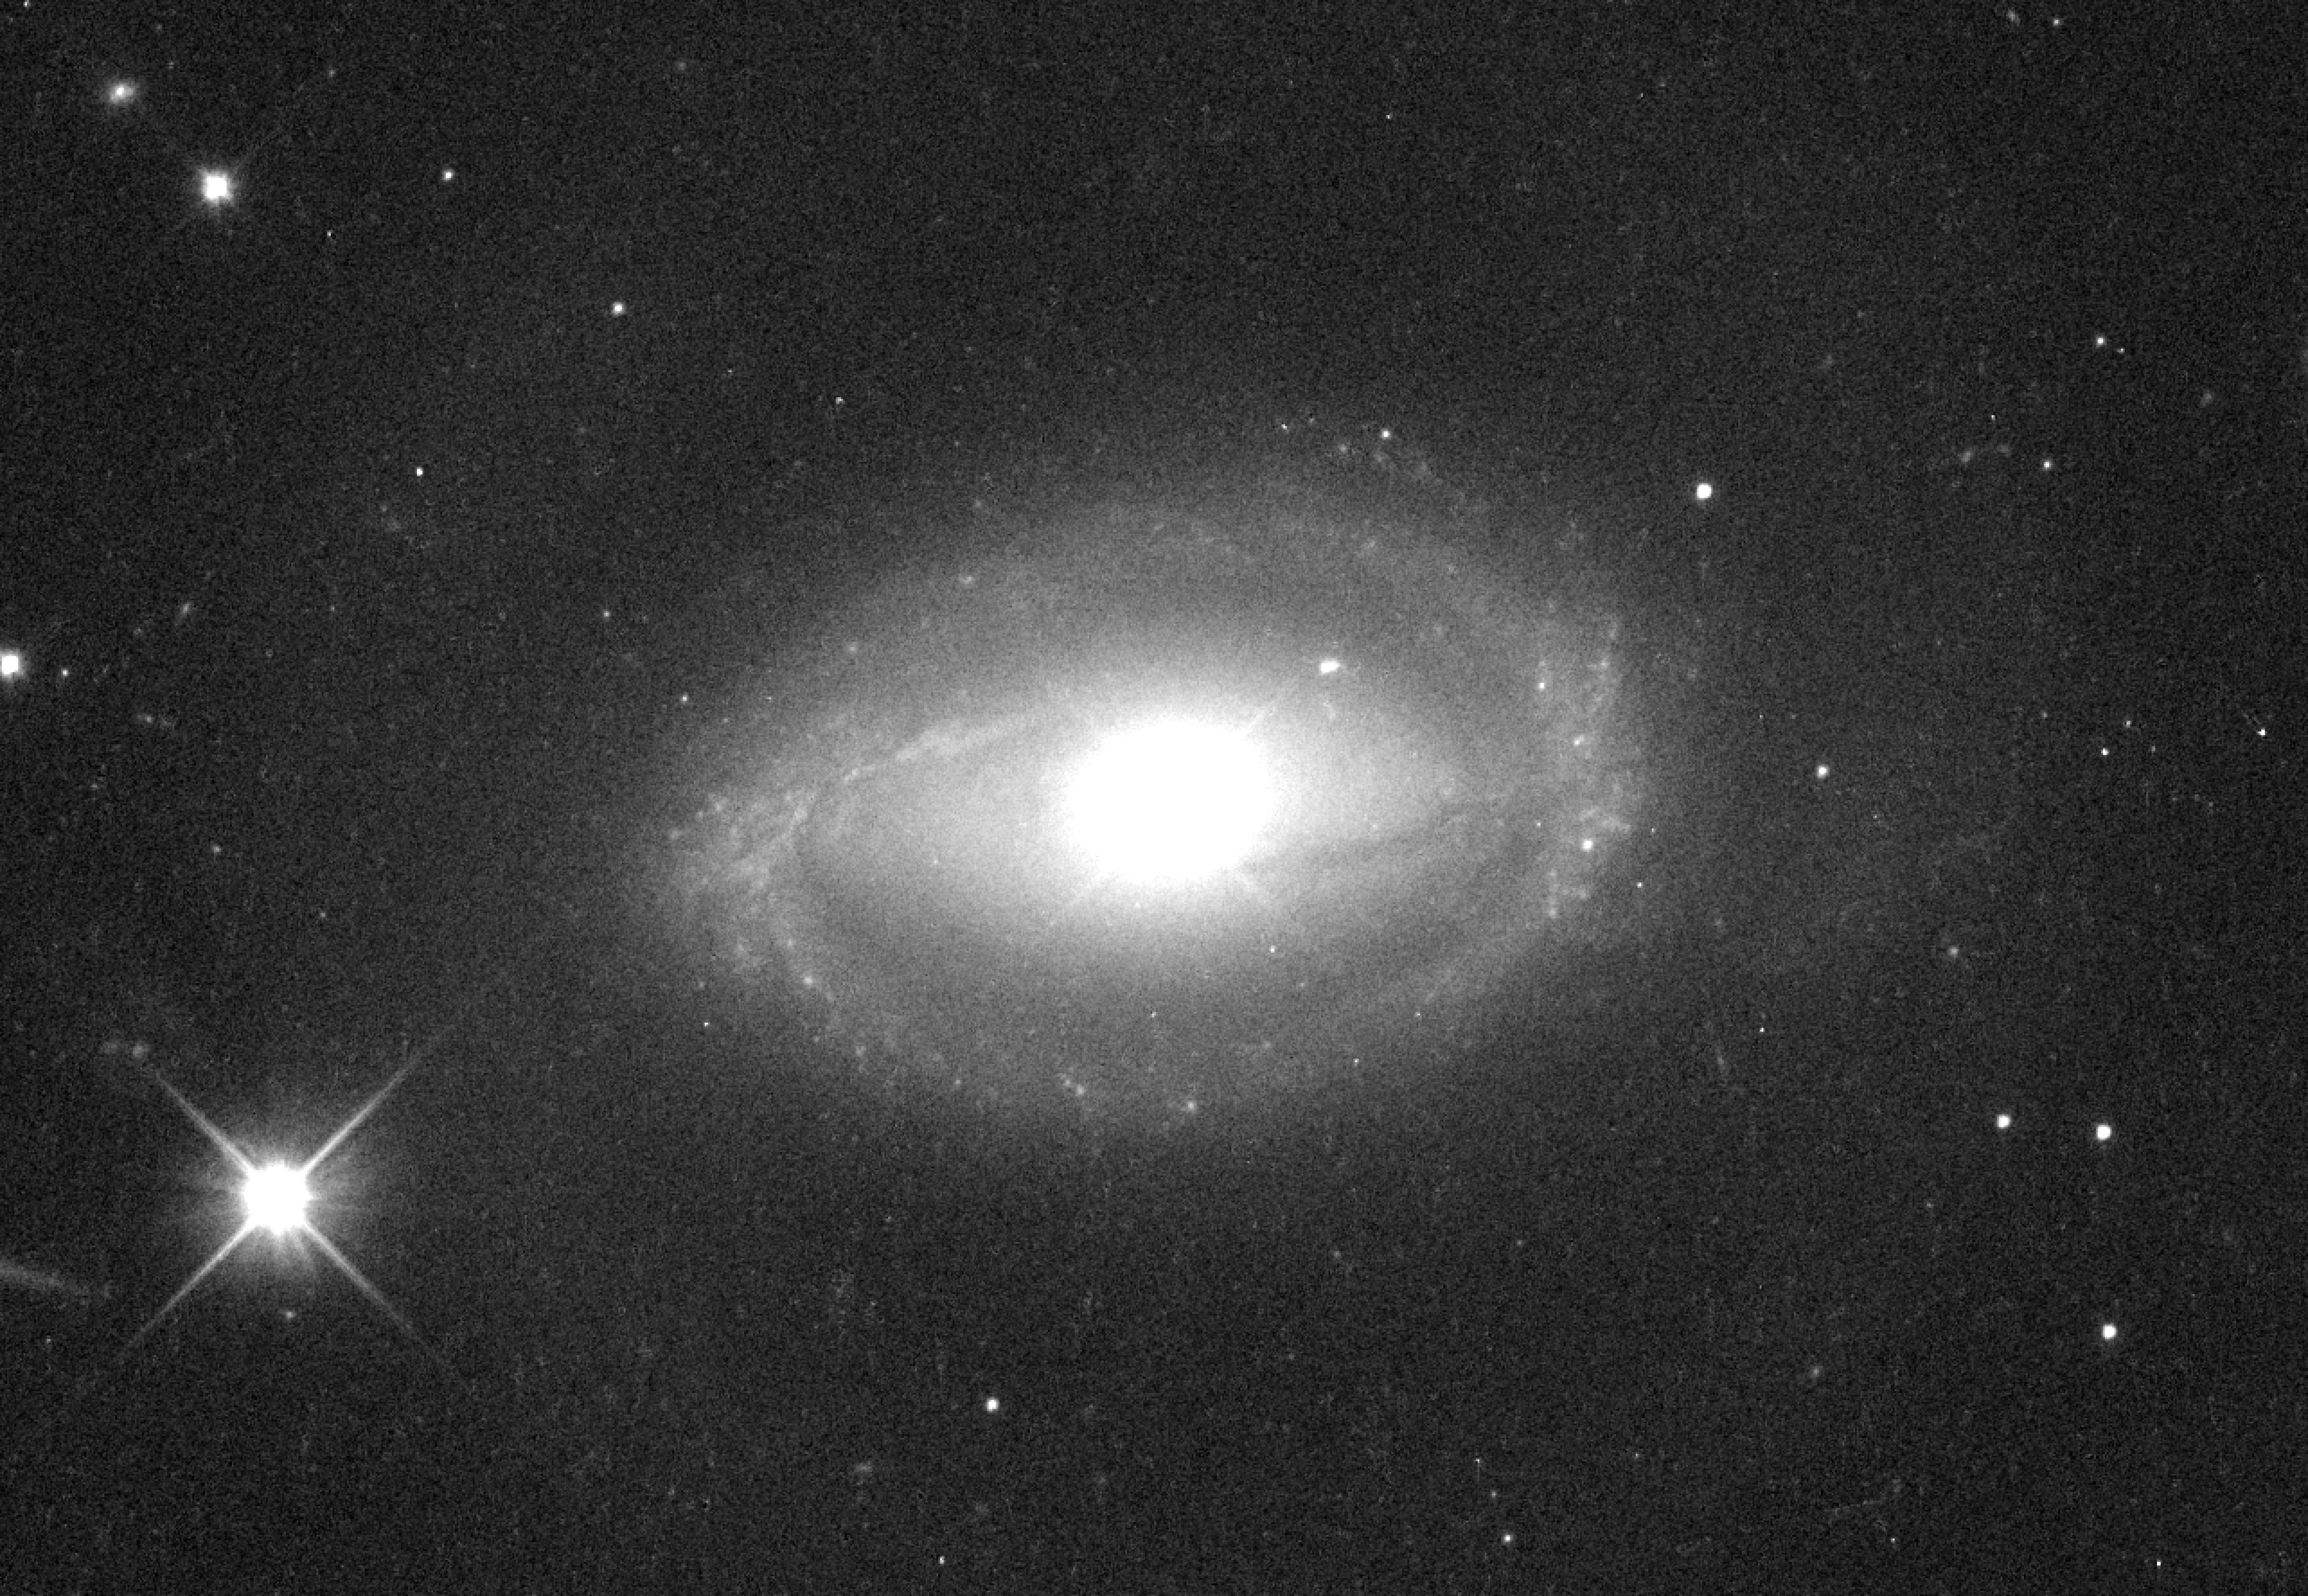
\includegraphics[scale=0.035]{images/Zw229-15_Crop.jpg}
  \end{figure}
  \begin{center}
    \href{https://archive.stsci.edu/}{{\tiny HST Image}}
  \end{center}
  \begin{columns}
    \begin{column}{0.5\textwidth}
      \begin{itemize}
        \item Sy 1 in Lyra
        \item $\Delta T_{H\beta} = 3.86^{+0.69}_{-0.90}$~d
      \end{itemize}
    \end{column}
    \begin{column}{0.5\textwidth}
      \begin{itemize}
        \item mag $15.4$
        \item $\mathrm{M}_{\mathrm{BH}} = 1.00^{+0.19}_{-0.24} \times 10^{7} \mathrm{M}_{\sun}$
      \end{itemize}
    \end{column}
  \end{columns}
  \begin{center}
    {\tiny \citep{Barth11}}
  \end{center}
\end{frame}

\begin{frame}
\frametitle{C-ARMA($2$,$1$) model of Zw 229-15\\Smoothed light curve}
  \begin{figure}
    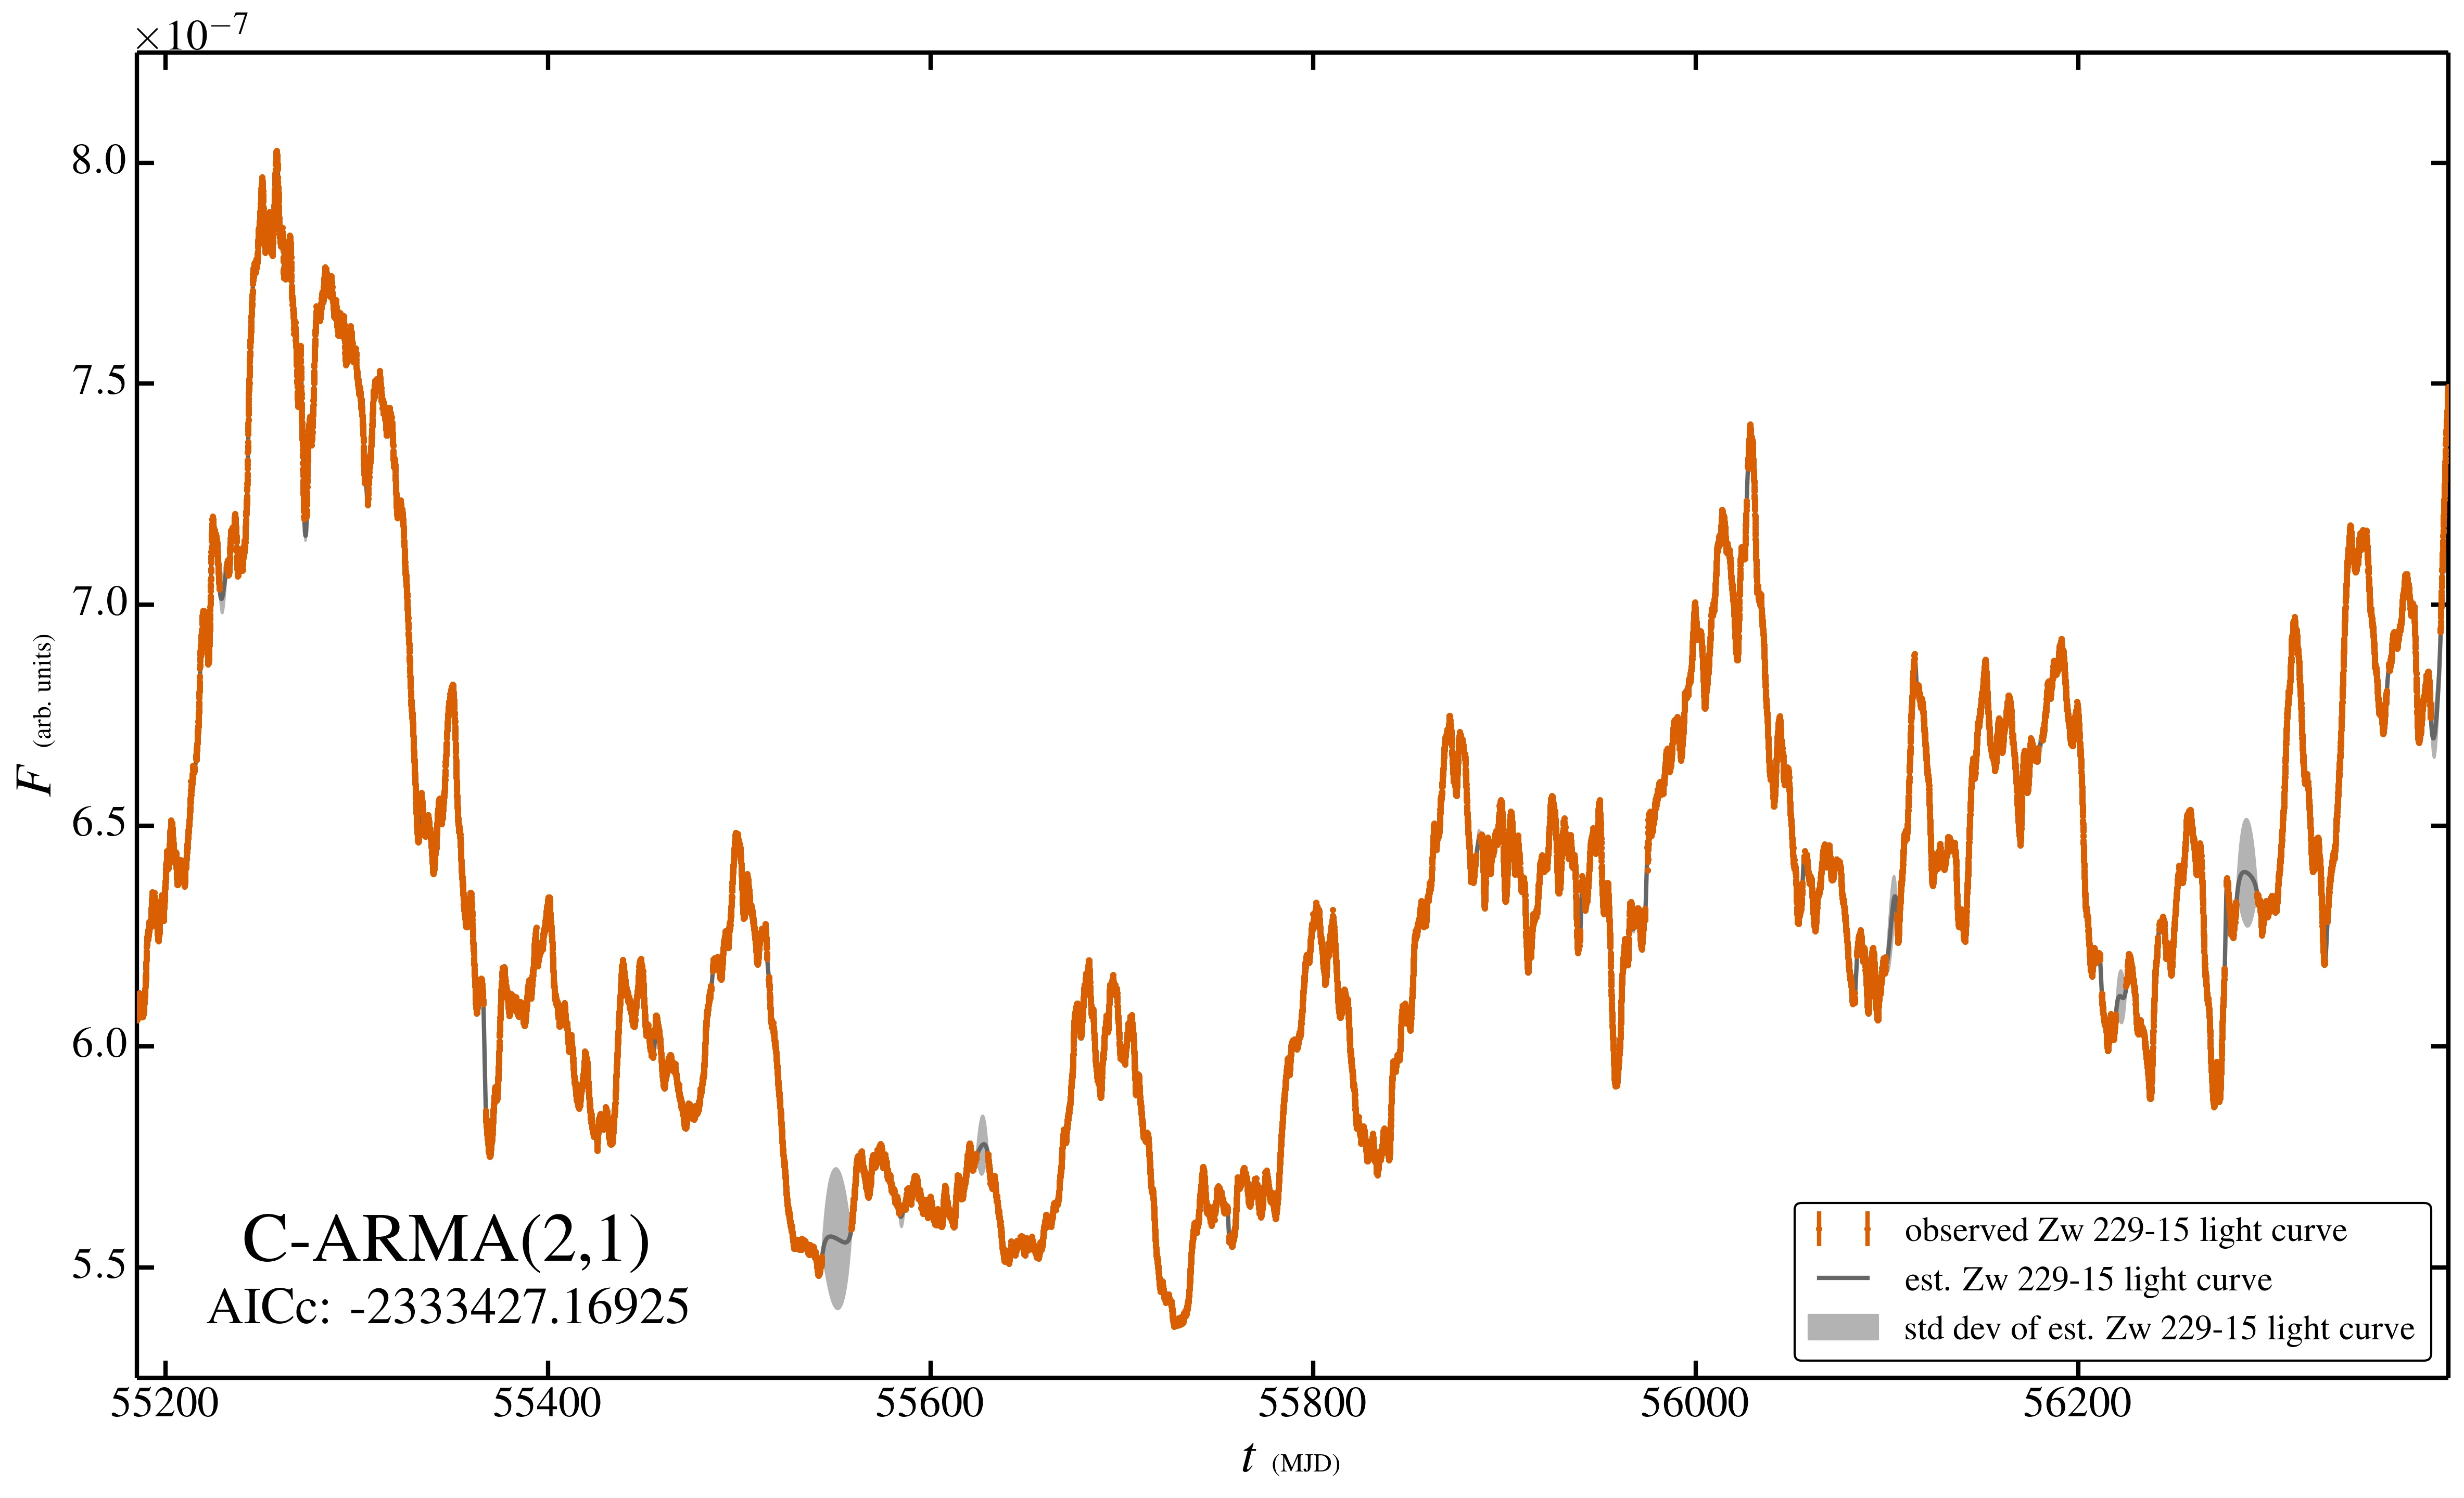
\includegraphics[scale=0.065]{images/Zw229-15_LC.jpg}
  \end{figure}
\end{frame}

\begin{comment}

\begin{frame}
\frametitle{C-ARMA($2$,$1$) model of Zw 229-15\\PSD of the light curve}
  \begin{figure}
    \includegraphics[scale=0.0725]{images/Periodogram+Fit.jpg}
  \end{figure}
\end{frame}

\begin{frame}
\frametitle{C-ARMA($2$,$1$) model of Zw 229-15\\Damped Harmonic Oscillator}
  \begin{figure}
    \includegraphics[scale=0.065]{images/Zw229-15_DampedHO.jpg}
  \end{figure}
\end{frame}


\end{comment}


\begin{frame}
\frametitle{C-ARMA($2$,$1$) model of Zw 229-15\\Green's Function}
  \begin{figure}
    \includegraphics[scale=0.065]{images/Zw229-15_GF.jpg}
  \end{figure}
\end{frame}


\begin{comment}


\begin{frame}
\frametitle{C-ARMA($2$,$1$) model of Zw 229-15\\Disturbance PSD}
  \begin{figure}
    \includegraphics[scale=0.065]{images/Zw229-15_distPSD.jpg}
  \end{figure}
\end{frame}

\begin{frame}
\frametitle{C-ARMA($2$,$1$) model of Zw 229-15\\Timescales}
  \begin{figure}
    \includegraphics[scale=0.055]{images/Zw229-15_Times.jpg}
  \end{figure}
\end{frame}

\begin{frame}
\frametitle{C-ARMA($2$,$1$) model of Zw 229-15\\Which is the real light curve?}
  \begin{figure}
    \includegraphics[scale=0.065]{images/Zw229-15_mockLC.jpg}
  \end{figure}
\end{frame}

\subsection{SDSS}

\begin{frame}
\frametitle{The Sloan Digital Sky Survey (SDSS)}
  \begin{center}
    \centering
        \begin{figure}
          \includegraphics[scale=0.25]{./images/SDSS.jpg}
        \end{figure}
  \end{center}
\end{frame}

\begin{frame}
\frametitle{Massive dataset from Stripe82}
  \begin{center}
    \centering
        \begin{figure}
          \includegraphics[scale=0.25]{./images/SDSSS82.jpg}
        \end{figure}
  \end{center}
\end{frame}

\begin{frame}
\frametitle{SDSS Photometric System}
  \begin{center}
    \centering
        \begin{figure}
          \includegraphics[scale=0.4]{./images/SDSSFilters.jpg}
        \end{figure}
  \end{center}
\end{frame}

\begin{frame}
\frametitle{Stripe 82 QSO C-ARMA fits}
  \begin{center}
    \centering
        \begin{figure}
          \includegraphics[scale=0.5]{./images/SDSSHist.jpg}
        \end{figure}
  \end{center}
  \begin{center}
    \href{http://www.drexel.edu/physics/research/researchAreas/Astrophysics/}{{\tiny Jack O'Brien}}
  \end{center}
\end{frame}

\begin{frame}
\frametitle{Work in Progress\\K2 campaigns}
        \begin{figure}
          \includegraphics[scale=0.325]{images/K2Campaigns.jpg}
        \end{figure}
\end{frame}


\end{comment}


\section{Ongoing Projects}

\subsection{Combing Surveys}

\begin{frame}
\frametitle{WiP: Power of SDSS+K2}
  \begin{figure}
    \includegraphics[scale=0.2]{images/LC_2.jpg}
  \end{figure}
  \begin{itemize}
    \item Spectra required for good colorterms
  \end{itemize}
\end{frame}

\begin{frame}
\frametitle{WiP: K2 observations of Stripe 82 QSOs}
  \begin{figure}
    \includegraphics[scale=0.05]{images/PowerOfSDSSK2.jpg}
  \end{figure}
  \begin{itemize}
    \item Prototype for LSST-DDF
    \item Can we use DASCH as well?
  \end{itemize}
\end{frame}


\begin{comment}


\begin{frame}
\frametitle{WiP: Beaming from Massive Black Hole Binaries\\{\tiny Inspired by \citet*{binarySMBHNature15}}}
        \begin{figure}
          \includegraphics[scale=0.05]{images/PowerOfSDSSK2.jpg}
        \end{figure}
  \begin{columns}
  \centering
    \begin{column}{0.5\textwidth}
      \begin{itemize}
        \item $M_{12} = 10^{9} M_{\sun}$
        \item $r_{\mathrm{peribothron}} = 0.01$ pc
        \item $T = 18.0$ yr
      \end{itemize}
    \end{column}
    \begin{column}{0.5\textwidth}
      \begin{itemize}
        \item $q = 0.1$
        \item $e = 0.7$
        \item $\omega$ \& $i = 90$ degree
      \end{itemize}
    \end{column}
  \end{columns}
\end{frame}

\begin{frame}
\frametitle{WiP: Effect on PSD}
\begin{columns}
\centering
  \begin{column}{0.5\textwidth}
    \begin{figure}
      \includegraphics[scale=0.04]{images/Ps_full.jpg}
    \end{figure}
  \end{column}
  \begin{column}{0.5\textwidth}
      \begin{figure}
        \includegraphics[scale=0.12]{images/Ps_detail.jpg}
      \end{figure}
  \end{column}
\end{columns}
\begin{columns}
\centering
  \begin{column}{0.5\textwidth}
    \begin{itemize}
      \item $a_{1} = 10^{-4}$ pc
      \item $a_{2} = 10^{-4}$ pc
      \item $T = 8.25$ d
      \item $e$ ranges from 0.0 to 0.75
    \end{itemize}
  \end{column}
  \begin{column}{0.5\textwidth}
    \begin{itemize}
      \item $M_{12} = 138.68 \times 10^{6} M_{\odot}$
      \item $\Omega = 0.0$ degree
      \item $i = 90.0$ degree
    \end{itemize}
  \end{column}
\end{columns}
\end{frame}


\end{comment}


\subsection{Toy Models of Massive Black Hole Binaries}

\begin{frame}
\frametitle{WiP: Is PG 1302-102 a Relativistically-Beamed \\ Massive Black Hole Binary?}
%\begin{columns}
%\centering
%  \begin{column}{0.5\textwidth}
  \begin{figure}
    \includegraphics[scale=0.05]{images/PG1302-102_LC.jpg}
  \end{figure}
  %\end{column}
  %\begin{column}{0.5\textwidth}
      %\begin{figure}
        %\includegraphics[scale=0.025]{images/PG1302-102_Fit.jpg}
      %\end{figure}
  %\end{column}
%\end{columns}
  \begin{columns}
  \centering
    \begin{column}{0.5\textwidth}
      \begin{itemize}
        \item {\scriptsize $a_{1} \sim 6.8 \times 10^{-3}$~pc}
        \item {\scriptsize $a_{2} \sim 1.1 \times 10^{-2}$~pc}
        \item {\scriptsize $T \sim 1343$~d}
      \end{itemize}
    \end{column}
    \begin{column}{0.5\textwidth}
      \begin{itemize}
        \item {\scriptsize $M_{12} \sim 4.05 \times 10^{9} M_{\odot}$}
        \item {\scriptsize $M_{2}/M_{1} \sim 0.66$}
        \item {\scriptsize $e \sim 0.077$}
      \end{itemize}
    \end{column}
  \end{columns}
\end{frame}

\section{The Road Goes Ever On And On...}

\subsection{Summary}

\begin{frame}
\frametitle{Work in Progress}
  \begin{columns}
    \centering
    \begin{column}{0.6\textwidth}
      \begin{itemize}
        \item SDSS Stripe 82 + K2 QSO variability
        \begin{itemize}
          \item Connection between AGN sub-type and variability
        \end{itemize}
        \item Detection of binary-SMBH via variability
        \item Better time series models for exotic objects (blazars)
        \item Cadence and periodicity requirements of LSST
        \item Multi-wavelength variability
        \item Comparing simulations with observations
        \item Stationarity of AGN light curves
      \end{itemize}
    \end{column}
    \begin{column}{0.4\textwidth}
        \begin{figure}
          \includegraphics[scale=0.25]{images/Hogg_lc.jpg}
        \end{figure}
        \begin{center}
          \href{https://www.astro.umd.edu/people/drewhogg.html}{{\tiny J. Drew Hogg}}
        \end{center}
    \end{column}
  \end{columns}
\end{frame}


\begin{comment}


\begin{frame}
\frametitle{Conclusions}
  \begin{itemize}
    \item Kepler AGN exhibit a \textbf{wide variety} of behavior (flares \& possibly QPOs)
    %\item PSD fits via monte carlo estimation of structure function
    \item DRW does \textbf{not work} for all AGN
    %\item Instrumentation \textbf{not responsible} for non-DRW behavior
    \item AGN variability can be modelled as a C-ARMA process
    %\item Kalman filter can be used to infer C-ARMA parameters
    %\item C-ARMA($2$,$1$) process is an \textbf{appropriate model} of variability for Zw 229-15
    \item Zw 229-15 acts like a \textbf{CARMA(2,1)} process (Damped Harmonic Oscillator Driven by Colored Noise)
    \item Relativistic-beaming from MBHB is \textbf{detectable} (un-realistic data quality is not a requirement!)
  \end{itemize}
\end{frame}


\end{comment}


\begin{frame}
\frametitle{LSST Prep}
  \begin{itemize}
    \item Learn as much as we can about the AGN in the DDF (we'll surely want spectra if nothing else).
    \item Determine single-band LSST sampling requirements {\scriptsize (J. Moreno)}.
      \begin{itemize}
        \item {\scriptsize Will the WFD survey be useful?}
        \item {\scriptsize Does adding DASCH \& TESS help?}
      \end{itemize}
    \item Test applicability of C-ARMA models to large sample of AGN {\scriptsize (J. Moreno, J. O'Brien, M. Graham \& others)}.
      \begin{itemize}
        \item {\scriptsize Can we make a strong case for tweaking the WFD survey to make it more useful?}
      \end{itemize}
    \item Probe connections between varibility properties \& physical properties {\scriptsize (J. O'Brien)}
      \begin{itemize}
        \item {\scriptsize Is variability a proxy for some other property?}
      \end{itemize}
    \item Develop models for multiplicative disturbances {\scriptsize (for blazars etc..)}.
    \item Develop \& test models for continuum-continuum variability.
      \begin{itemize}
        \item {\scriptsize How much does taking data non-simultaneously hurt us?}
      \end{itemize}
  \end{itemize}
\end{frame}


\begin{comment}

\begin{frame}
\frametitle{ARMA Stochastic Processes}
  \begin{equation*} w_{k} \sim \mathcal{N}(0,\sigma^{2}) \end{equation*}
  \begin{equation*} F_{k} = \phi_{1} F_{k - 1} + \ldots + \phi_{p} F_{k - p} + w_{k} + \theta_{1} w_{k - 1} + \ldots + \theta_{q} w_{k - q} \end{equation*}
  \begin{columns}
    \centering
    \begin{column}{0.5\textwidth}
      \begin{itemize}
        \item Auto-Regressive Moving Average process {\tiny \citet{BrockwellDavisITSF}}
        \item PSD: rational function - arbitarily complex
        \item Not continuous!
        \item $F_{i} = 1.25F_{i-1} - 0.3F_{i-2} + w_{i}$, $w \sim \mathcal{N}(0,2)$
      \end{itemize}
    \end{column}
    \begin{column}{0.5\textwidth}
      \begin{figure}
        \includegraphics[scale=0.035]{../images/talk/ARMA(2,0)_Master.jpg}
      \end{figure}
    \end{column}
  \end{columns}
\end{frame}

\section{Modelling AGN Variability as a C-ARMA Process}

\subsection{Introduction}

\begin{frame}
\frametitle{Continuous-time AutoRegressive Moving Average (C-ARMA) Processes}
  \begin{equation*} \mathrm{d}W \sim \mathcal{N}(0,\mathrm{d}t) \end{equation*}
  \begin{equation*}\label{eq:CARMA} \mathrm{d}^{p}x + \alpha_{1} \mathrm{d}^{p-1}x + \ldots + \alpha_{p-1} \mathrm{d}x + \alpha_{p}x = \beta_{0} (\mathrm{d}W) + \ldots + \beta_{q} \mathrm{d}^{q}(\mathrm{d}W) \end{equation*}
  \begin{columns}
    \centering
    \begin{column}{0.5\textwidth}
      \begin{itemize}
        \item Uses It\={o} calculus {\tiny \citet{Brockwell14,Davis,Kelly14}}
        \item LHS comes from linear perturbations of non-linear system
        \item C-ARMA $\overset{\mathrm{sample}}\longrightarrow$ ARMA
        \item PSD is a ratio of even polynomials in frequency
      \end{itemize}
    \end{column}
    \begin{column}{0.5\textwidth}
      \begin{figure}
        \includegraphics[scale=0.0425]{images/CARMA(3,1)_LC.jpg}
        %${\scriptstyle \mathrm{d}^{2}f + 0.7 \mathrm{d}f + 0.011f = 7.0 \times 10^{-9} (\mathrm{d}W) + 1.2 \times 10^{-9} \mathrm{d}(\mathrm{d}W)}$
      \end{figure}
    \end{column}
  \end{columns}
\end{frame}

\begin{frame}
\frametitle{Power Spectral Density\\Eg. C-ARMA($2$,$1$)}
  %\begin{equation*}\label{eq:CARMA21PSD} \mathrm{d}^{2}F + 2\omega\zeta \mathrm{d}F + \omega^{2}F = \beta_{1} \mathrm{d}(\mathrm{d}W) + \beta_{2} (\mathrm{d}W) \end{equation*}
  \begin{columns}
    \begin{column}{0.5\textwidth}
      \begin{figure}
        \includegraphics[scale=0.04]{images/CARMA(2,1)_PSD.jpg}
      \end{figure}
    \end{column}
    \begin{column}{0.5\textwidth}
      \begin{figure}
        \includegraphics[scale=0.04]{images/CARMA(2,1)_LC.jpg}
      \end{figure}
    \end{column}
  \end{columns}
  %\begin{center}
  %{\tiny \citet*{Kasliwal15b}}
  %\end{center}
\end{frame}

\begin{frame}
\frametitle{Power Spectral Density\\Eg. C-ARMA($5$,$1$)}
  %\begin{equation*}\label{eq:CARMA21PSD} \mathrm{d}^{2}F + 2\omega\zeta \mathrm{d}F + \omega^{2}F = \beta_{1} \mathrm{d}(\mathrm{d}W) + \beta_{2} (\mathrm{d}W) \end{equation*}
  \begin{columns}
    \begin{column}{0.5\textwidth}
      \begin{figure}
        \includegraphics[scale=0.04]{images/CARMA(5,1)_PSD.jpg}
      \end{figure}
    \end{column}
    \begin{column}{0.5\textwidth}
      \begin{figure}
        \includegraphics[scale=0.04]{images/CARMA(5,1)_LC.jpg}
      \end{figure}
    \end{column}
  \end{columns}
  %\begin{center}
  %{\tiny \citet*{Kasliwal15b}}
  %\end{center}
\end{frame}

\subsection{State-Space Representation}

\begin{frame}
\frametitle{State Space Representation}
%\begin{equation*}\label{eq:1stCanForm}
%\mathbfss{A} = \left( \begin{array}{ccccc}
%-\alpha_{1} & 1 & \hdots & 0 & 0 \\
%-\alpha_{2} & 0 & \hdots & 0 & 0 \\
%\vdots & \vdots & \ddots & \vdots & \vdots \\
%-\alpha_{p-1} & 0 & \hdots & 0 & 1 \\
%-\alpha_{p} & 0 & \hdots & 0 & 0 \\
%\end{array}\right); \mathbfit{B} = \left( \begin{array}{c} \beta_{1} \\ \beta_{2} \\ \vdots \\ \beta_{p-1} \\ \beta_{p} \end{array} \right); \mathbfss{H} = \left( \begin{array}{c} 1 \\ 0 \\ \vdots \\ 0 \\ 0 \end{array} \right)^{\top}.
%\end{equation*}

  %\begin{equation*}\label{eq:StateEqn} \mathrm{d}\mathbfit{x} = \mathbfss{A}\mathbfit{x}\mathrm{d}t + \mathbfit{B}\mathrm{d}w \end{equation*}
  %\begin{equation*}\label{eq:ObsEqn} y = \mathbfss{H}\mathbfit{x} \end{equation*}

  %\begin{equation*}\label{eq:TransMat} \mathbfss{F} = \mathrm{e}^{\mathbfss{A}\delta t} \end{equation*}
  %\begin{equation*}\label{eq:DistMat} \mathbfss{Q} = \int_{0}^{\delta t} \mathrm{e}^{\mathbfss{A}\xi}\mathbfit{B}\mathbfit{B}^{\top}\mathrm{e}^{\mathbfss{A}^{\top}\xi} d\xi \end{equation*}

  State equation: \begin{equation*}\label{eq:ARMAStateEq} \mathbfit{x}_{k+1} = \mathbfss{F}\mathbfit{x}_{k} + \mathbfit{w}_{k} \end{equation*} \begin{equation*}\label{eq:ARMADisturbance} \mathbfit{w}_{k} \sim \mathcal{N}(\mathbfit{0},\mathbfss{Q}) \end{equation*}

  Observation equation: \begin{equation*}\label{eq:ARMAObsEqn} x_{k, \mathrm{obs}} = \mathbfss{H}_{k}\mathbfit{x}_{k} + v_{k} \end{equation*} \begin{equation*}\label{eq:ARMANoise} v_{k} \sim \mathcal{N}(0,\sigma^{2}_{N,k}) \end{equation*}

  \begin{itemize}
    \item $\mathbfss{F}$: Transition matrix \& $\mathbfss{Q}$: Disturbance matrix
    \item $\mathbfss{H}$: Observation matrix
    \item Observation noise in-built via $v_{k}$!
    \item Well studied by engineers (Control systems) and economists
  \end{itemize}
\end{frame}

\begin{frame}
\frametitle{Evolution \& observation of light curve state}
  \begin{center}
    \centering
    \movie[externalviewer]{\includegraphics[scale=0.2]{images/Fig0_Pt5_Step4.jpg}}{LC2.mp4}
        %\href{http://168.176.8.14/sagan/TipoAGN.html}{{\tiny Columbian National University: Bogota}}
  \end{center}
  %\begin{center}
    %\centering
    %{\tiny \citet{ArmitageReynolds03}}
  %\end{center}
\end{frame}

\begin{comment}

\begin{frame}
\frametitle{A C-ARMA(2,1) light curve}
  \begin{figure}
    \includegraphics[scale=0.05]{images/CARMA(2,2)_Master.jpg}
  \end{figure}
\end{frame}

\subsection{The Kalman Filter}

\begin{frame}
\frametitle{$\ln \mathcal{L}$ via Kalman filter}
  \begin{center}
    \centering
    \movie[externalviewer]{\includegraphics[scale=0.2]{images/Fig1_Pt5_Step5.jpg}}{LnLike2.mp4}
        %\href{http://168.176.8.14/sagan/TipoAGN.html}{{\tiny Columbian National University: Bogota}}
  \end{center}
  %\begin{center}
    %\centering
    %{\tiny \citet{ArmitageReynolds03}}
  %\end{center}
\end{frame}

\begin{frame}
\frametitle{Confidence Interval Estimates}
  \begin{figure}
    \includegraphics[scale=0.075]{images/CARMA(2,1)_Recovery.jpg}
  \end{figure}
\end{frame}

\begin{comment}

\begin{frame}
\frametitle{Smoothed Light Curve}
  \begin{figure}
    \includegraphics[scale=0.0725]{images/CARMA(2,2)_MCMCFit.jpg}
  \end{figure}
\end{frame}

\begin{frame}
\frametitle{How to Interpret?: Green's Function of LHS\\(eg. C-ARMA($2$,$1$)...)}
  \begin{equation*}\label{eq:CARMAGF} \mathrm{d}^{2}G + 2\omega\zeta \mathrm{d}G + \omega^{2}G = \delta(0) \end{equation*}
  \begin{figure}
    \includegraphics[scale=0.06]{images/CARMA(2,1)_GF.jpg}
  \end{figure}
  %\begin{center}
  %{\tiny \citet*{Kasliwal15b}}
  %\end{center}
\end{frame}

\subsection{C-ARMA Analysis of Zw 229-15}

\begin{frame}
\frametitle{Zw 229-15 (kplr006932990)}
  \begin{figure}
    \includegraphics[scale=0.035]{images/Zw229-15_Crop.jpg}
  \end{figure}
  \begin{center}
    \href{https://archive.stsci.edu/}{{\tiny HST Image}}
  \end{center}
  \begin{columns}
    \begin{column}{0.5\textwidth}
      \begin{itemize}
        \item Sy 1 in Lyra
        \item $\Delta T_{H\beta} = 3.86^{+0.69}_{-0.90}$~d
      \end{itemize}
    \end{column}
    \begin{column}{0.5\textwidth}
      \begin{itemize}
        \item mag $15.4$
        \item $\mathrm{M}_{\mathrm{BH}} = 1.00^{+0.19}_{-0.24} \times 10^{7} \mathrm{M}_{\sun}$
      \end{itemize}
    \end{column}
  \end{columns}
  \begin{center}
    {\tiny \citep{Barth11}}
  \end{center}
\end{frame}

\begin{frame}
\frametitle{C-ARMA($2$,$1$) model of Zw 229-15\\Smoothed light curve}
  \begin{figure}
    \includegraphics[scale=0.065]{images/Zw229-15_LC.jpg}
  \end{figure}
\end{frame}

\begin{comment}

\begin{frame}
\frametitle{C-ARMA($2$,$1$) model of Zw 229-15\\PSD of the light curve}
  \begin{figure}
    \includegraphics[scale=0.0725]{images/Periodogram+Fit.jpg}
  \end{figure}
\end{frame}

\begin{frame}
\frametitle{C-ARMA($2$,$1$) model of Zw 229-15\\Damped Harmonic Oscillator}
  \begin{figure}
    \includegraphics[scale=0.065]{images/Zw229-15_DampedHO.jpg}
  \end{figure}
\end{frame}

\begin{frame}
\frametitle{C-ARMA($2$,$1$) model of Zw 229-15\\Green's Function}
  \begin{figure}
    \includegraphics[scale=0.065]{images/Zw229-15_GFunc.jpg}
  \end{figure}
\end{frame}

\begin{frame}
\frametitle{C-ARMA($2$,$1$) model of Zw 229-15\\Disturbance PSD}
  \begin{figure}
    \includegraphics[scale=0.065]{images/Zw229-15_distPSD.jpg}
  \end{figure}
\end{frame}

\begin{frame}
\frametitle{C-ARMA($2$,$1$) model of Zw 229-15\\Timescales}
  \begin{figure}
    \includegraphics[scale=0.055]{images/Zw229-15_Times.jpg}
  \end{figure}
\end{frame}

\begin{frame}
\frametitle{C-ARMA($2$,$1$) model of Zw 229-15\\Which is the real light curve?}
  \begin{figure}
    \includegraphics[scale=0.065]{images/Zw229-15_mockLC.jpg}
  \end{figure}
\end{frame}

\subsection{SDSS}

\begin{frame}
\frametitle{The Sloan Digital Sky Survey (SDSS)}
  \begin{center}
    \centering
        \begin{figure}
          \includegraphics[scale=0.25]{../images/talk/SDSS.jpg}
        \end{figure}
  \end{center}
\end{frame}

\begin{frame}
\frametitle{Massive dataset from Stripe82}
  \begin{center}
    \centering
        \begin{figure}
          \includegraphics[scale=0.25]{../images/talk/SDSSS82.jpg}
        \end{figure}
  \end{center}
\end{frame}

\begin{frame}
\frametitle{SDSS Photometric System}
  \begin{center}
    \centering
        \begin{figure}
          \includegraphics[scale=0.4]{../images/talk/SDSSFilters.jpg}
        \end{figure}
  \end{center}
\end{frame}

\begin{frame}
\frametitle{Stripe 82 QSO C-ARMA fits}
  \begin{center}
    \centering
        \begin{figure}
          \includegraphics[scale=0.5]{../images/talk/SDSSHist.jpg}
        \end{figure}
  \end{center}
  \begin{center}
    \href{http://www.drexel.edu/physics/research/researchAreas/Astrophysics/}{{\tiny Jack O'Brien}}
  \end{center}
\end{frame}

\section{WIP \& Summary}

\subsection{Work in Progress}

\begin{frame}
\frametitle{Work in Progress\\K2 campaigns}
        \begin{figure}
          \includegraphics[scale=0.325]{images/K2Campaigns.jpg}
        \end{figure}
\end{frame}

\begin{frame}
\frametitle{Work in Progress\\K2 observations of Stripe 82 QSOs}
        \begin{figure}
          \includegraphics[scale=0.25]{images/LC_2.jpg}
        \end{figure}
\end{frame}

\begin{frame}
\frametitle{Work in Progress}
  \begin{columns}
    \centering
    \begin{column}{0.6\textwidth}
      \begin{itemize}
        \item SDSS Stripe 82 + K2 QSO variability
        \item Connection between AGN sub-type and variability
        \item Stationarity of AGN light curves
        \item More sophisticated time series models
        \item Comparing simulations with observations
        \item Cadence and periodicity requirements of LSST
        \item Multi-wavelength variability
        \item Detection of binary-SMBH via variability
      \end{itemize}
    \end{column}
    \begin{column}{0.4\textwidth}
        \begin{figure}
          \includegraphics[scale=0.25]{images/Hogg_lc.jpg}
        \end{figure}
        \begin{center}
          \href{https://www.astro.umd.edu/people/drewhogg.html}{{\tiny J. Drew Hogg}}
        \end{center}
    \end{column}
  \end{columns}
\end{frame}

\subsection{Summary}

\begin{frame}
\frametitle{Conclusions}
  \begin{itemize}
    \item Kepler AGN exhibit a \textbf{wide variety} of behavior (flares \& possibly QPOs)
    %\item PSD fits via monte carlo estimation of structure function
    \item DRW does \textbf{not work} for all AGN
    %\item Instrumentation \textbf{not responsible} for non-DRW behavior
    \item AGN variability can be modelled as a C-ARMA process
    \item Kalman filter can be used to infer C-ARMA parameters
    \item C-ARMA($2$,$1$) process is an \textbf{appropriate model} of variability for Zw 229-15
    \item Zw 229-15 acts like a \textbf{Damped Harmonic Oscillator Driven by Colored Noise}
  \end{itemize}
\end{frame}


\begin{frame}
\frametitle{Acknowledgements}
  This work has been supported by NASA Grant NNX14AL56G. I would like
  to thank the following people for their help \& support:
  \begin{itemize}
    \item Advisor: Dr. Michael S. Vogeley
    \item Co-Advisor: Dr. Gordon T. Richards
    \item Collaborator: Dr. Michael T. Carini
    \end{itemize}
  \begin{columns}
    \begin{column}{0.5\textwidth}
      \begin{itemize}
        \item Dr. Robert Gilmore
        \item Dr. John Walsh
        \item Jackeline Moreno
        \item Jack O'Brien
      \end{itemize}
    \end{column}
    \begin{column}{0.5\textwidth}
      \begin{itemize}
        \item Dr. Michel Valli\'{e}res
        \item Dr Stephen McMillan
        \item Dr. Dave Goldberg
        \item (Dr.) Frank Jones
      \end{itemize}
    \end{column}
  \end{columns}
\end{frame}

\end{comment}

\appendix
\begin{frame}[allowframebreaks]
  \bibliography{../TeX/bibliography/allrefs}
\end{frame}

\begin{comment}

\subsection{Extra Slides: Researcher's Cut}

\begin{frame}
\frametitle{AGN sample}
  \begin{columns}
    \centering
    \begin{column}{0.65\textwidth}
      \begin{figure}
        \includegraphics[scale=0.2]{../images/talk/kplr012158940_LC.jpg}
        %\caption{Light curve of kplr012158970, a Type 1 Seyfert.}
      \end{figure}
    \end{column}
    \begin{column}{0.35\textwidth}
        \begin{itemize}
        %\item kplr012158970
        \item Seyfert 1
        %\item $z = 0.067$.
        \item $\delta t_{\mathrm{rest}} \sim 27.5$~min
        \item $N \sim 50$k
          %\pause
        \item Stationary?
        \end{itemize}
    \end{column}
  \end{columns}
\end{frame}

\begin{frame}
\frametitle{AGN sample}
  \begin{columns}
    \centering
    \begin{column}{0.65\textwidth}
      \begin{figure}
        \includegraphics[scale=0.2]{../images/talk/kplr002694186_LC.jpg}
        %\caption{Light curve of kplr003347632, a Type 2 Seyfert.}
      \end{figure}
    \end{column}
    \begin{column}{0.35\textwidth}
        \begin{itemize}
        %\item kplr003347632
        \item Seyfert 1
        %\item $z = 0.089$.
        \item $\delta t_{\mathrm{rest}} \sim 27.0$~min
        \item $N \sim 44$k
          %\pause
        \item QPO?
        \end{itemize}
    \end{column}
  \end{columns}
\end{frame}

\begin{frame}
\frametitle{AGN sample}
  \begin{columns}
    \centering
    \begin{column}{0.65\textwidth}
      \begin{figure}
        \includegraphics[scale=0.2]{../images/talk/kplr006690887_LC.jpg}
        %\caption{Light curve of kplr010663134, a FSRQ.}
      \end{figure}
    \end{column}
    \begin{column}{0.35\textwidth}
        \begin{itemize}
        %\item kplr010663134
        \item BL Lacertae object
        %\item $z = 1.52$.
        \item $\delta t_{\mathrm{rest}} \sim 25.5$~min
        \item $N \sim 28$k
          %\pause
        \item Flares!
        \end{itemize}
    \end{column}
  \end{columns}
\end{frame}

\begin{frame}
\frametitle{Monte-Carlo simulations}
  \begin{figure}
    \includegraphics[scale=0.15]{images/kplr012158940_Fit.jpg}
  \end{figure}
  \begin{itemize}
    \centering
    \item Best-fit Parameters: $\gamma = 2.54$ \& $\tau = 40.2$~d
    \item Inconsistent with DRW ($\gamma_{DRW} = 2$)
    \item $\chi^{2}$ of best-fit PSD model $> 71.3$\% of mocks
    \end{itemize}
\end{frame}

\begin{frame}
\frametitle{Monte-Carlo simulations}
  \begin{figure}
    \includegraphics[scale=0.15]{images/kplr002694186_Fit.jpg}
  \end{figure}
  \begin{itemize}
    \centering
    \item Best-fit Parameters: $\gamma = 2.09$ \& $\tau = 134.3$~d
    \item Consistent with DRW ($\gamma_{DRW} = 2$)
    \item $\chi^{2}$ of best-fit PSD model $> 88.6$\% of mocks
    \end{itemize}
\end{frame}

\begin{frame}
\frametitle{Monte-Carlo simulations}
  \begin{figure}
    \includegraphics[scale=0.15]{images/kplr006690887_Fit.jpg}
  \end{figure}
  \begin{itemize}
    \centering
    \item Best-fit Parameters: $\gamma = 2.25$ \& $\tau = 3.0$~d
    \item Not well-modelled by a DRW ($\gamma_{DRW} = 2$)
    \item $\chi^{2}$ of best-fit PSD model $> 99.9$\% of mocks
    \end{itemize}
\end{frame}

\begin{frame}
\frametitle{SDSS light curves}
  \begin{center}
    \centering
        \begin{figure}
          \includegraphics[scale=0.05]{../images/talk/SDSS_LC.jpg}
        \end{figure}
  \end{center}
  \begin{columns}
    \begin{column}{0.5\textwidth}
      \centering
      \begin{itemize}
        \item Large dataset ($\sim 10000$ AGN)
        \item Well-characterized photometry
      \end{itemize}
    \end{column}
    \begin{column}{0.5\textwidth}
      \centering
      \begin{itemize}
        \item Long temporal baseline ($\sim 10$~yr)
        \item Sparse sampling
      \end{itemize}
    \end{column}
  \end{columns}
\end{frame}

\begin{frame}
\frametitle{\citet{Macleod10}: Apply DRW to SDSS QSOs}
  \begin{columns}
    \begin{column}{0.5\textwidth}
      \begin{center}
        \begin{figure}
          \includegraphics[scale=1.5]{../images/talk/Macleod10b.jpg}
        \end{figure}
      \end{center}
    \end{column}
    \begin{column}{0.5\textwidth}
        \begin{figure}
          \includegraphics[scale=1.75]{../images/talk/Macleod10a.jpg}
        \end{figure}
    \end{column}
  \end{columns}
  %\centering
  %{\tiny \citet{Kelly09}}
  \begin{itemize}
    \item Thermal processes responsible for variability
    \item No `evolution' over cosmic time.
    \item $\tau \sim \mathrm{M}_{\mathrm{BH}}$ but not $L_{\mathrm{AGN}}$
  \end{itemize}
\end{frame}

\begin{frame}
\frametitle{Photometer Design}
  \begin{center}
    \centering
        \begin{figure}
          \includegraphics[scale=0.55]{../images/talk/Kepler_Photometer.jpg}
        \end{figure}
  \end{center}
\end{frame}

\begin{frame}
\frametitle{Optical Layout}
  \begin{center}
    \centering
        \begin{figure}
          \includegraphics[scale=0.65]{../images/talk/Kepler_OpticalDesign.jpg}
        \end{figure}
  \end{center}
\end{frame}

\begin{frame}
\frametitle{Kepler Focal Plane}
  \begin{center}
    \centering
        \begin{figure}
          \includegraphics[scale=0.65]{../images/talk/Kepler_FocalPlane.jpg}
        \end{figure}
  \end{center}
\end{frame}

\begin{frame}
\frametitle{Kepler Focal Plane Layout}
  \begin{center}
    \centering
        \begin{figure}
          \includegraphics[scale=0.5]{../images/talk/Kepler_FocalPlaneLayout.jpg}
        \end{figure}
  \end{center}
\end{frame}

\begin{frame}
\frametitle{Kepler Bandpass}
  \begin{center}
    \centering
        \begin{figure}
          \includegraphics[scale=0.65]{../images/talk/Kepler_SpectralResponse.jpg}
        \end{figure}
  \end{center}
\end{frame}

\begin{frame}
\frametitle{Kepler PRF \& Chromatic aberration}
  \begin{center}
    \centering
        \begin{figure}
          \includegraphics[scale=0.5]{../images/talk/Kepler_PRF.jpg}
        \end{figure}
        \begin{figure}
          \includegraphics[scale=0.5]{../images/talk/Kepler_ChromaticAberration.jpg}
        \end{figure}
  \end{center}
\end{frame}

\begin{frame}
\frametitle{Kepler Image Quality}
  \begin{center}
    \centering
        \begin{figure}
          \includegraphics[scale=0.65]{../images/talk/Kepler_StellarDensity.jpg}
        \end{figure}
  \end{center}
\end{frame}

\begin{frame}
\frametitle{Artifact: FGS Crosstalk (Dark)}
  \begin{center}
    \centering
        \begin{figure}
          \includegraphics[scale=0.35]{../images/talk/Kepler_FGSCrosstalk.jpg}
        \end{figure}
  \end{center}
\end{frame}

\begin{frame}
\frametitle{Artifact: Video Crosstalk}
  \begin{center}
    \centering
        \begin{figure}
          \includegraphics[scale=0.65]{../images/talk/Kepler_VideoCrosstalk.jpg}
        \end{figure}
  \end{center}
\end{frame}

\begin{frame}
\frametitle{Artifact: Start-of-Line Ringing (SOLR)}
  \begin{center}
    \centering
        \begin{figure}
          \includegraphics[scale=0.35]{../images/talk/Kepler_StartOfLineRinging.jpg}
        \end{figure}
  \end{center}
\end{frame}

\begin{frame}
\frametitle{Artifact: Undershoot}
  \begin{center}
    \centering
        \begin{figure}
          \includegraphics[scale=0.35]{../images/talk/Kepler_FGSCrosstalk_Undershoot.jpg}
        \end{figure}
  \end{center}
\end{frame}

\begin{frame}
\frametitle{Artifact: Rolling Bands}
  \begin{center}
    \centering
        \begin{figure}
          \includegraphics[scale=0.35]{../images/talk/Kepler_RollingBand.jpg}
        \end{figure}
  \end{center}
\end{frame}

\begin{frame}
\frametitle{Artifact: Moire Pattern Drift (MPD)}
  \begin{center}
    \centering
        \begin{figure}
          \includegraphics[scale=0.65]{../images/talk/Kepler_MPD.jpg}
        \end{figure}
  \end{center}
\end{frame}

\begin{frame}
\frametitle{Artifact: Bright Star Induced MPD}
  \begin{center}
    \centering
        \begin{figure}
          \includegraphics[scale=0.65]{../images/talk/Kepler_BrightStarMPD.jpg}
        \end{figure}
  \end{center}
\end{frame}

\begin{frame}
\frametitle{Kepler Mission}
  \begin{center}
    \centering
        \begin{figure}
          \includegraphics[scale=0.1]{../images/talk/Kepler_TransitMethod.jpg}
        \end{figure}
  \end{center}
  \begin{columns}
    \begin{column}{0.5\textwidth}
      \begin{itemize}
        \item Required precision $\sim 20$~ppm
        \item Desired lifetime $\sim 4$~yr
      \end{itemize}
    \end{column}
    \begin{column}{0.5\textwidth}
      \begin{itemize}
        \item Achieved precision $\sim 35$~ppm
        \item Actual lifetime $\sim 3.5$~yr
      \end{itemize}
    \end{column}
  \end{columns}
  \begin{center}
    {\tiny \citet{Gilliland11,DR24}}
  \end{center}
\end{frame}

\begin{frame}
\frametitle{Offsets}
  \begin{columns}
    \centering
    \begin{column}{0.6\textwidth}
      \begin{figure}
        \includegraphics[scale=0.2]{../images/talk/Stitching.jpg}
      \end{figure}
    \end{column}
   \begin{column}{0.4\textwidth}
       \begin{itemize}
       \item Inter-quarter
       \item Photometric aperture re-definition
       \item Stitching: End-match mean ($100$ obs)
       \end{itemize}
    \end{column}
  \end{columns}
\end{frame}

\begin{frame}
\frametitle{Crowding}
  \begin{figure}
    \includegraphics[scale=0.35]{../images/talk/kplr006932990-Q7_Heatmap.jpg}
  \end{figure}
  \begin{center}
    \href{http://www.drexel.edu/physics/contact/graduate/Moreno\ Jackeline/}{{\tiny Jackeline Moreno}}
  \end{center}
\end{frame}

\begin{frame}
\frametitle{Disturbance PSD\\C-ARMA($2$,$1$) case}
  \begin{equation*}\label{eq:CARMAdPSD} u = \beta_{1} \mathrm{d}(\mathrm{d}W) + \beta_{2} (\mathrm{d}W) \end{equation*}
  \begin{figure}
    \includegraphics[scale=0.06]{../images/talk/CARMA(2,1)_distPSD.jpg}
  \end{figure}
  %\begin{center}
  %{\tiny \citet*{Kasliwal15b}}
  %\end{center}
\end{frame}

\begin{frame}
\frametitle{State Space Representation}
%\begin{equation*}\label{eq:1stCanForm}
%\mathbfss{A} = \left( \begin{array}{ccccc}
%-\alpha_{1} & 1 & \hdots & 0 & 0 \\
%-\alpha_{2} & 0 & \hdots & 0 & 0 \\
%\vdots & \vdots & \ddots & \vdots & \vdots \\
%-\alpha_{p-1} & 0 & \hdots & 0 & 1 \\
%-\alpha_{p} & 0 & \hdots & 0 & 0 \\
%\end{array}\right); \mathbfit{B} = \left( \begin{array}{c} \beta_{1} \\ \beta_{2} \\ \vdots \\ \beta_{p-1} \\ \beta_{p} \end{array} \right); \mathbfss{H} = \left( \begin{array}{c} 1 \\ 0 \\ \vdots \\ 0 \\ 0 \end{array} \right)^{\top}.
%\end{equation*}

  %\begin{equation*}\label{eq:StateEqn} \mathrm{d}\mathbfit{x} = \mathbfss{A}\mathbfit{x}\mathrm{d}t + \mathbfit{B}\mathrm{d}w \end{equation*}
  %\begin{equation*}\label{eq:ObsEqn} y = \mathbfss{H}\mathbfit{x} \end{equation*}

  %\begin{equation*}\label{eq:TransMat} \mathbfss{F} = \mathrm{e}^{\mathbfss{A}\delta t} \end{equation*}
  %\begin{equation*}\label{eq:DistMat} \mathbfss{Q} = \int_{0}^{\delta t} \mathrm{e}^{\mathbfss{A}\xi}\mathbfit{B}\mathbfit{B}^{\top}\mathrm{e}^{\mathbfss{A}^{\top}\xi} d\xi \end{equation*}

  State equation: \begin{equation*}\label{eq:ARMAStateEq} \mathbfit{x}_{k+1} = \mathbfss{F}\mathbfit{x}_{k} + \mathbfit{w}_{k} \end{equation*}

  Observation equation: \begin{equation*}\label{eq:ARMAObsEqn} y_{k} = \mathbfss{H}_{k}\mathbfit{x}_{k} + v_{k} \end{equation*}

  Disturbance \& noise properties
  \begin{equation*}\label{eq:ARMADisturbance} \mathbfit{w}_{k} \sim \mathcal{N}(\mathbfit{0},\mathbfss{Q}) \end{equation*}
  \begin{equation*}\label{eq:ARMANoise} v_{k} \sim \mathcal{N}(0,\sigma^{2}_{N,k}) \end{equation*}
\end{frame}

\begin{frame}
\frametitle{Evolution \& observation of light curve state}
  \begin{figure}
    \includegraphics[scale=0.2]{../images/talk/Fig0_Pt5_Step1.jpg}
  \end{figure}
  %\begin{center}
  %{\tiny \citet*{Kasliwal15b}}
  %\end{center}
\end{frame}

\begin{frame}
\frametitle{Evolution \& observation of light curve state\\Evolution without disturbance}
  \begin{figure}
    \includegraphics[scale=0.2]{../images/talk/Fig0_Pt5_Step2.jpg}
  \end{figure}
  %\begin{center}
  %{\tiny \citet*{Kasliwal15b}}
  %\end{center}
\end{frame}

\begin{frame}
\frametitle{Evolution \& observation of light curve state\\Effect of the disturbance}
  \begin{figure}
    \includegraphics[scale=0.2]{../images/talk/Fig0_Pt5_Step3.jpg}
  \end{figure}
  %\begin{center}
  %{\tiny \citet*{Kasliwal15b}}
  %\end{center}
\end{frame}

\begin{frame}
\frametitle{Evolution \& observation of light curve state\\Observing the AGN}
  \begin{figure}
    \includegraphics[scale=0.2]{../images/talk/Fig0_Pt5_Step4.jpg}
  \end{figure}
  %\begin{center}
  %{\tiny \citet*{Kasliwal15b}}
  %\end{center}
\end{frame}

\begin{frame}
\frametitle{$\ln \mathcal{L}$ via Kalman filter}
  \begin{figure}
    \includegraphics[scale=0.2]{../images/talk/Fig1_Pt5_Step1.jpg}
  \end{figure}
  %\begin{center}
  %{\tiny \citet*{Kasliwal15b}}
  %\end{center}
\end{frame}

\begin{frame}
\frametitle{$\ln \mathcal{L}$ via Kalman filter\\Predict Step}
  \begin{figure}
    \includegraphics[scale=0.2]{../images/talk/Fig1_Pt5_Step2.jpg}
  \end{figure}
  %\begin{center}
  %{\tiny \citet*{Kasliwal15b}}
  %\end{center}
\end{frame}

\begin{frame}
\frametitle{$\ln \mathcal{L}$ via Kalman filter\\Innovation calculation}
  \begin{figure}
    \includegraphics[scale=0.2]{../images/talk/Fig1_Pt5_Step3.jpg}
  \end{figure}
  %\begin{center}
  %{\tiny \citet*{Kasliwal15b}}
  %\end{center}
\end{frame}

\begin{frame}
\frametitle{$\ln \mathcal{L}$ via Kalman filter\\Update $\ln \mathcal{L}$}
  \begin{figure}
    \includegraphics[scale=0.2]{../images/talk/Fig1_Pt5_Step4.jpg}
  \end{figure}
  %\begin{center}
  %{\tiny \citet*{Kasliwal15b}}
  %\end{center}
\end{frame}

\begin{frame}
\frametitle{$\ln \mathcal{L}$ via Kalman filter\\Correct Step}
  \begin{figure}
    \includegraphics[scale=0.2]{../images/talk/Fig1_Pt5_Step5.jpg}
  \end{figure}
  %\begin{center}
  %{\tiny \citet*{Kasliwal15b}}
  %\end{center}
\end{frame}

\begin{frame}
\frametitle{MCMC Estimation}
  \begin{figure}
    \includegraphics[scale=0.0725]{../images/talk/CARMA(2,2)_Walkers.jpg}
  \end{figure}
\end{frame}

\begin{frame}
\frametitle{Large Scale Structure of the Universe}
  \begin{center}
    \centering
        \begin{figure}
          \includegraphics[scale=0.1]{../images/talk/SDSSLSS.jpg}
        \end{figure}
  \end{center}
\end{frame}

\begin{frame}
\frametitle{Ivezi\'{c} Stripe 82 Calibration}
  \begin{center}
    \centering
        \begin{figure}
          \includegraphics[scale=0.3]{../images/talk/SDSSCalibration.jpg}
        \end{figure}
  \end{center}
  \begin{center}
    \href{http://www.drexel.edu/physics/research/researchAreas/Astrophysics/}{{\tiny Jack O'Brien}}
  \end{center}
\end{frame}

\begin{frame}
\frametitle{Stripe 82 QSO C-ARMA fits}
  \begin{center}
    \centering
        \begin{figure}
          \includegraphics[scale=0.3]{../images/talk/SDSSHists.jpg}
        \end{figure}
  \end{center}
  \begin{center}
    \href{http://www.drexel.edu/physics/research/researchAreas/Astrophysics/}{{\tiny Jack O'Brien}}
  \end{center}
\end{frame}

\begin{frame}
\frametitle{Stripe 82 QSO\\Effect of Ivezi\'{c} calibration}
  \begin{center}
    \centering
        \begin{figure}
          \includegraphics[scale=0.4]{../images/talk/SDSSCalibrationEffect.jpg}
        \end{figure}
  \end{center}
  \begin{center}
    \href{http://www.drexel.edu/physics/research/researchAreas/Astrophysics/}{{\tiny Jack O'Brien}}
  \end{center}
\end{frame}

\begin{frame}
\frametitle{Stripe 82 QSO light curve C-ARMA fit}
  \begin{center}
    \centering
        \begin{figure}
          \includegraphics[scale=0.3]{../images/talk/SDSSFit.jpg}
        \end{figure}
      \centering
      C-ARMA($3$,$1$) $\rightarrow$ C-ARMA($2$,$1$)
  \end{center}
  \begin{center}
    \href{http://www.drexel.edu/physics/research/researchAreas/Astrophysics/}{{\tiny Jack O'Brien}}
  \end{center}
\end{frame}

\begin{frame}
\frametitle{Work in Progress\\K2}
        \begin{figure}
          \includegraphics[scale=0.055]{../images/talk/K2.jpg}
        \end{figure}
\end{frame}

\end{comment}

\end{document}
